\documentclass[a4paper]{article}

\usepackage{newtxtext} \usepackage{newtxmath}
\usepackage{graphicx}
\graphicspath{ {../Images/} }
\usepackage[utf8]{inputenc}
\usepackage[T1]{fontenc}
\usepackage{textcomp}
\usepackage{amssymb}
\usepackage{amsmath, amssymb}
\newtheorem{problem}{Problem}
\newtheorem{example}{Example}
\newtheorem{lemma}{Lemma}
\newtheorem{theorem}{Theorem}
\newtheorem{problem}{Problem}
\newtheorem{example}{Example} \newtheorem{definition}{Definition}
\newtheorem{lemma}{Lemma}
\newtheorem{theorem}{Theorem}
\usepackage{parskip}

\begin{document}
    

\begin{titlepage}
   \begin{center}
       \vspace*{1cm}

       \textbf{Matemática Discreta II}

       \small
       \vspace{0.5cm}
        FAMAF - UNC
            
       \vspace{1.5cm}
       \footnotesize
       \textbf{Severino Di Giovanni}
       \normalsize

       \vfill
            
            
     
   \end{center}
\end{titlepage}

 \begin{figure}[h!]
 \centering
  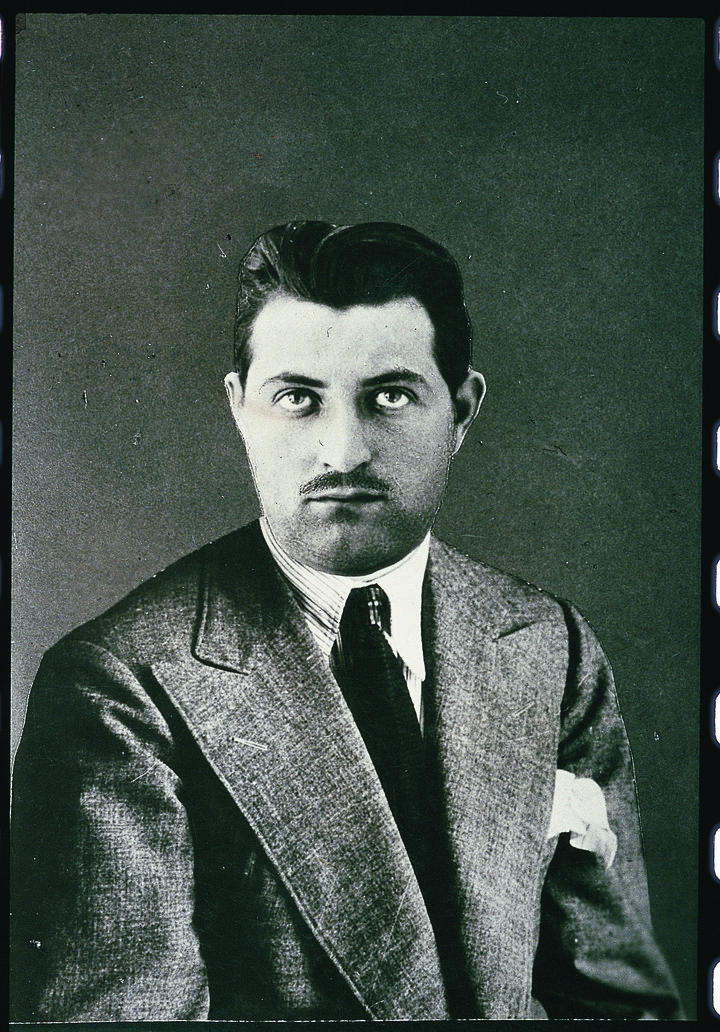
\includegraphics[width=0.5\textwidth]{../Images/SeverinoDiGiovanni.jpg}
 \caption{Severino Di Giovanni, el autor de este apunte. Un anarquista
   libertario, murió luchando por la libertad. Como él, otros miles han muerto
   para que nosotros gocemos de los derechos que tenemos. No te dejes engañar
   por los tristes pregoneros del egoísmo. Amá a tu prójimo y no olvides que si
   sus derechos se vulneran, los tuyos también. Ayudá a tu compañero de estudio,
 defendé tu universidad. }
 \end{figure}

\pagebreak

\tableofcontents
\newpage

\section{Grafos}

\subsection{Info de la materia}

\textit{Mail del profesor.} daniel.penazzi@unc.edu.ar

\textit{Temas a ver.}

\begin{itemize}
    \item Coloreo de grafos 
    \item Flujos en network 
    \item Matchings 
    \item Códigos de correción de errores
    \item P-NP (Complejidad computacional)
    \item Inteligencia artifical
\end{itemize}

La materia tiene tres partes: teórico, práctico y proyecto de programación. Solo
la parte práctica tiene promoción (se explica abajo). El final tiene parte
teórica y parte práctica. La parte teórica es demostrar uno de tres teoremas
dados a priori. La parte práctica tiene ejercicios de demostración o pensamiento
y de resolución de problemas.

La parte práctica se promociona si se aprueban los dos parciales, con cualquer
nota $\geq 4$. De promocionarlo, la parte práctica del final no es necesaria.

El proyecto de programación tiene dos partes. La primera es leer un grafo y
cargar los datos al programa. La segunda es un problema de coloreo de grafos. La
fecha de entrega de la parte uno es en dos o tres semanas a partir de hoy
(13/03). La parte importante es la parte 2.

La biliografía está en el programa 2023.

\subsection{Grafos}

\begin{definition}
    Una grafo es una $2$-upla $G = (V, E)$ con $V$ un conjunto cualquiera (finito) y $E
    \subseteq \left\{ A \subseteq V : |A| = 2 \right\} $
\end{definition}


\small
\begin{quote}

\textbf{Nota.} La restricción de finitud es sólo de esta materia. 

\end{quote}
\normalsize

\begin{center}
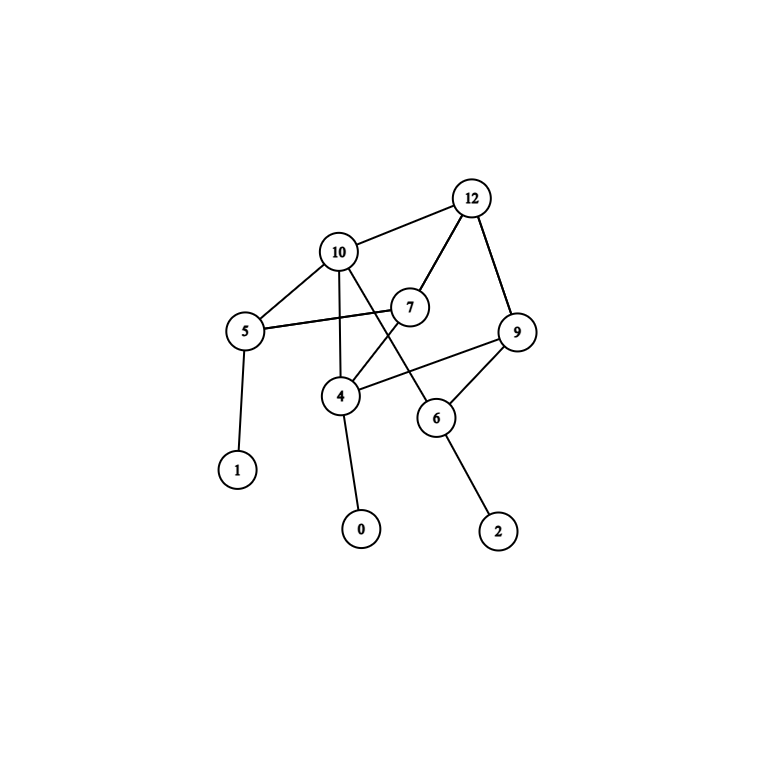
\includegraphics[scale=0.5]{graph}
\end{center}

Los elementos de $V$ se llaman vértices o nodos. Los elementos de $E$ se llaman
lados o aristas. Por convención, a menos que digamos lo contrario, es que $|V| =
n$ y $|E| = m$.

\begin{definition}
    Un camino en un grafo $G = (V, E) $ es una sucesión de vértices $v_1,
    \ldots, v_r$, con $ v_i \in V$ para todo $i$, tal que $\left\{ v_j, v_{j+1}
    \right\} \in E $ para todo $1 \leq j < r$. 
\end{definition}


Dado un camino $v_1, \ldots, v_r$, si $v_1 = x, v_r = y$, decimos que es un
camino de $x$ a $y$. Para todo $G = (V, E)$ definimos la relación binaria 

$$\sim ~:=\left\{ (x, y) \in V^2 : \text{ existe un camino de $x$ a $y$ }  \right\} $$

Es decir, $x \sim y$ denota la relación de que existe un camino entre $x$ e $y$.
Es trivial comproabar que $\sim$ es una relación de equivalencia. Cada clase de
equivalencia $a / \sim$ con $a \in V$ se llama una componente conexa de $G$.

\begin{definition}
    Decimos que $G = (V, E) $ es conexo si y solo si tiene una sola componente
    conexa. Es decir, si $|V / \sim | = 1$.
\end{definition}


\small
\begin{quote}

El profesor no mencionó esto pero es lindo recordar (si alguien ha cursado
lógica) que el conjunto de clases de equivalencia $A / R$ de un conjunto a sobre
una relación binaria $R$ puede en sí mismo darse como un grupo de grafos
disconexos. Por ejemplo, abajo se dan los grafos de un espacio cociente con
siete clases de equivalencia; cada par de vértices unidos por un lado
corresponde a dos elementos equivalentes.


\begin{center}
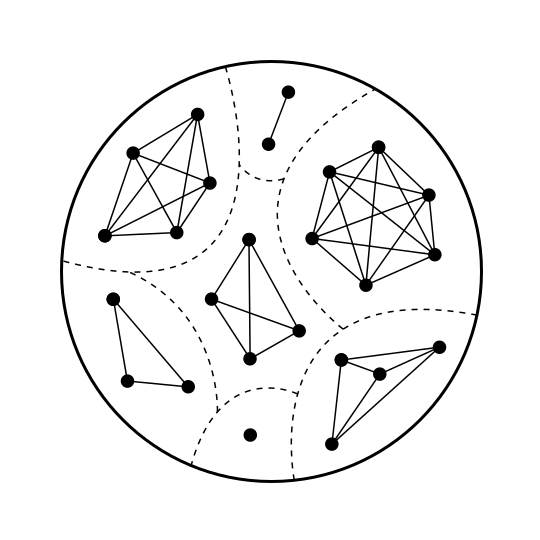
\includegraphics[scale=0.25]{equiv}
\end{center}

Fíjense que de esto se sigue un dato curioso (aunque tal vez irrelevante): Si
$G = (V, E) $ es un grafo conexo con $n$ vértices, el grafo que describe la clase de
equivalencia de $V$ es $K_n$.

\end{quote}
\normalsize

\begin{definition}
    Decimos que un grafo $H = (W, F)$ es un subgrafo de $G =(V, E)$ si
    $W \subseteq V, F \subseteq E$.
\end{definition}

A veces usamos $H \subseteq G$ para decir "$H$ es un subgrafo de $G$", pero no
debe entenderse por esto que $H$ y $G$ son conjuntos.

Observe que no todo $W \subseteq V, F \subseteq E$ satisfacen que $(W, F)$ es un
grafo. Por ejemplo, si $F = \emptyset$ tenemos $F \subseteq E$, pero $F$
no cumple la propiedad de que todos sus elementos sean conjuntos con cardinalidad $2$.

\begin{definition}[Densidad]
    Decimos que un grafo es denso si $m = O(n^2)$. Decimos que un grafo es raro
    si $m = O(n)$.
\end{definition}


\small
\begin{quote}

\textbf{Random fact}. Recuerde que "raro" no sólo significa "inusual" sino que es el
antónimo de "denso". La etimología inglesa es más interesante:
La palabra \textit{Weird} (raro) significaba, en la edad media, destino. Por
eso, en la balada medieval \textit{True Thomas}, se lee "Weird shall never
daunton me": El destino nunca ha de asustarme. Se debe a una antigua leyenda
nórdica en la cual las \textit{Weird sisters}, diosas terribles, tejían el
destino de los hombres. Si le da curiosidad:

https://en.wikipedia.org/wiki/Three_Witches

\end{quote}
\normalsize

\begin{definition}
    Dado $G = (V, E) $, si $x \in V$, $\Gamma(x) := \left\{ y \in V : \left\{ x,
        y\right\}  \in E
\right\} $ se llama el vecindario de $x$. 
\end{definition}

Si $y \in \Gamma(x)$, decimos que $y$
es un vecino de $x$.  El grado de $x$, denotado $d(x)$, es la cantidad de
vecinos de $x$; es decir, $d(x) = |\Gamma(x)|$.
Usamos $\delta = \min \left\{ d(x) : x \in V \right\} $ y $\Delta = \max \left\{
d(x) : x \in V\right\} $. Si $\delta = \Delta$ se dice que $G$ es regular. Por
ejemplo, los
grafos cíclicos y los completos son regulares.

\begin{definition}
    Dado un grafo $G = (V, E) $, decimos que $G$ es regular si $d(x) = d(y)$
    para todo $x, y \in V$.
\end{definition}

Es decir, un grafo es regular si todo vértice tiene la misma cantidad de
vecinos.



\subsection{Repaso de BFS y DFS}

\textit{A completar.}






\subsection{Los grafos $K_n$ y $C_n$}
\label{famosos}

\begin{itemize}
    \item $K_n$ : El grafo completo en $n$ vértices se define 

        $$K_n = \left( \left\{
        1, 2, \ldots, n\right\}, \left\{ \left\{ x, y \right\}  : x, y \in \left\{ 1, 2, \ldots, n
    \right\}  \right\}   \right) $$

    Es el grafo de $n$ elementos donde todos los vértices están conectados unos
    con otros. Resulta que que $m = \binom{n}{2}$. Lo cual implica que $m =
    O(n^2)$.

    \item  $C_n$: El grafo cíclico 

        $$C_n = \left( \left{ 1, 2, \ldots, n \right},
        \left\{ 12, 23, 34, \ldots, (n-1)n, n1 \right\}   \right)$$

        Una observación es
        que $C_3 = K_3$; pero de allí en adelante difieren.
\end{itemize}

\subsection{Coloreo de grafos}

\begin{definition}
    Un coloreo propio de $G = (V, E) $ con $k$ colores es una función  

    \begin{align*}
        C : V \mapsto A
    \end{align*}

    con $|A| = k$ y tal que $xy \in A\Rightarrow C(x) \neq C(y)$.
\end{definition}

Intuitivamente, un coloreo asigna $k$ propiedades a los vértices de modo tal que
ningún par de grafos adyacentes cumple la misma propiedad. 

\small
\begin{quote}

\textbf{Nota.} Hace unos meses escrbí un algoritmo de coloreo en C. Es el
segundo algoritmo dado en esta entrada: 

https://slopezpereyra.github.io/2023-10-29-Hamiltonian/

No prometo que sea muy prolijo o esté bien explicado; ya en general uno es tonto
y encima de tonto no sabe de grafos. Pero tal vez a alguien le sirva, qué se yo.

\end{quote}
\normalsize


\begin{definition}
    El número cromático de un grafo $G= (V, E) $ es 

    \begin{align*}
        \chi(G) = \min_k \left( \exists \text{ coloreo propio de $G$ con $k$
        colores} \right) 
    \end{align*}
\end{definition}

No se conoce un algoritmo polinomial que calcule $\chi(G)$. El proyecto será dar
un algoritmo polinomial que se aproxime a $\chi$.

\subsection{Un algoritmo greedy de coloreo}
~ ~ 

Damos un algoritmo que colorea un grafo $G$ con vértices $v_1, \ldots, v_n$ y
colores $ c_1, c_2, \ldots, c_n  $. Para que el algoritmo
funcione, los colores y los vértices deben tener un orden (en nuestro caso
dado por los subíndices).


\begin{quote}

\textbf{Invariante del algoritmo.} Los coloreos parciales son propios. Es decir,
a medida que se va coloreando iterativamente el grafo, en cada paso el coloreo
resultante debe ser propio.

\textbf{Pasos del algoritmo}. 

\textit{(1)} $C(v_1) = c_1$.

\textit{(2)} $C(v_k) = $ mínimo color que mantenga un coloreo propio (que
satisfaga el invariante).

\end{quote}


\begin{center}
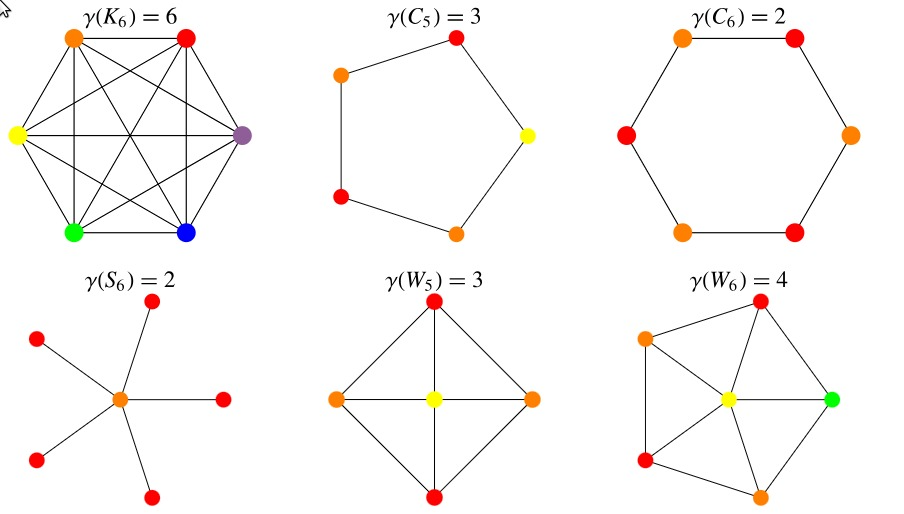
\includegraphics[scale=0.35]{coloring}
\end{center}

\subsection{Acotando $\chi$}

Generalmente nos interesa encontar $\chi(G)$ dado un grafo $G = (V, E) $. Damos
unas pautas y observaciones generales para acotar $\chi(G)$ y así facilitar su
hallazgo.

\begin{lemma}
    Si existe un coloreo propio de $G = (V, E)$ con $k$ colores, entonces
    $\chi(G) \leq k$.
\end{lemma}


\small
\begin{quote}

\textbf{Proof.} Es trivial por definición de $\chi$ ($\chi$ es el mínimo $k$ en
el conjunto de los coloreos posibles de $G$ con $k$ colores).

\end{quote}
\normalsize

El lema significa que para acotar $\chi$ por arriba solo basta dar un coloreo
con $k$ colores.

\begin{lemma}
    Si $H$ es un subgrafo de $G$, $\chi(H) \leq \chi(G)$.
\end{lemma}

Este lema nos dice que podemos acotar $\chi$ por abajo si encontramos un
subgrafo de $G$ cuyo número cromático es conocido. Es fácil ver que $\chi(K_r) =
r$ para todo $r > 1$. Es menos directo pero en clase se demostró que

\begin{align*}
    \chi(C_r) = \begin{cases}
        2 & r \equiv 0 \mod 2  \\ 
        3 & r \equiv 1 \mod 2 
    \end{cases}
\end{align*}

Esto, en combinación con el último lema, nos dice que podemos acotar $\chi(G)$
por abajo simplemente observando si $G$ contiene algún $C_r$  o $K_r$ como
subgrafo. En el caso $C_r$, la cota inferior dada en el caso par, con $\chi(C_r)
= 2$, es trivial (todo grafo necesita al menos dos colores). Por eso nos
quedamos con el siguiente teorema: 

\begin{theorem}
    Sea $G = (V, E) $ un grafo. Si $C_r \subseteq G$ con $r$ impar entonces
    $\chi(G) \geq 3$. Si $K_r \subseteq G$ entonces $\chi(G) \geq r$.
\end{theorem}

\begin{theorem}
    
    Sea $G = (V, E) $ un grafo. Entonces 

    $$\chi(G) = \max \left\{ \chi(C) : C \text{ es componente
conexa de  } G \right\} $$

\end{theorem}


\begin{theorem}
    Sea $G = (V, E) $ un grafo. Entonces $G$ contiene un ciclo impar si y solo
    si $\chi(G) \geq 3$.
\end{theorem}

\small
\begin{quote}

\textbf{Proof.} $(\Rightarrow)$ Trivial. 

$(\Leftarrow)$ Damos una prueba algorítmica. La prueba es simple, pero debe
tenerse presente que usamos \textbf{tres} grafos diferentes en ella: el grafo
$G = (V, E) $ del teorema, una componente conexa $C \subseteq G$, y un grafo
$\mathcal{B} \subseteq C$ resultante de correr BFS de a partir de un vértice de
$C$. El algoritmo determina si $\chi(G) = 2$ y de no serlo construye un ciclo
impar. Usamos la notación $n(z)$ si $z \in V$ para denotar el nivel de $z$ en
$\mathcal{B}$. Dividimos la prueba en tres partes.

\textit{(1)} Como $\chi(G) = \max \left\{ \chi(C) : C \text{ es componente
conexa de  } G \right\} $, tenemos que 

\begin{align*}
    \chi(G) \geq 3 \Rightarrow\exists \text{ c.c. $C$ tal que } \chi(C) \geq 3
\end{align*}

Elegimos $x \in C$ y corremos BFS a partir de él, generando un subgrafo
$\mathcal{B} \subseteq C$ con todos los vértices de $C$ (pero no todos los
lados).

\textit{(2)} Coloreamos cada vértice de $C$ como sigue: como sigue: $c(z)$ será el nivel
BFS de $z$ módulo 2. Esto equivale a hacer $c(x) = 0$ y cada vez que $y$ agrega
a $z$ a la cola de BFS, hacer $c(z) =  1 - c(y)$.

Esto da un coloreo con $2$ colores, pero podría no ser propio (por ejemplo, dos
vecinos de la raíz que son vecinos entre sí tendrían ambos color $1$). Por lo
tanto verificamos si es propio o no. 

\textit{(3)} Si es propio tenemos un coloreo propio de dos colores y $\chi(G) =
2$. Si es impropio, construiremos un ciclo impar. En particular, si no es
propio, existen $u, v \in V$ tales que $c(u) = c(v) $ y $uv \in E$. Pero si
$c(u) = c(v)$, entonces

\begin{align*}
    n(u) \equiv n(v) \mod 2
\end{align*}

Pero en un árbol siempre existe un camino
de la raíz a cualquier vértice arbitrario. Entonces, en $\mathcal{B}$ existe un
camino desde $x$ hasta $u$, y existe un camino desde $x$ hasta $v$. En
particular, existe un vértice $z$ que está en ambos caminos y a partir del cual
los caminos se separan (note que puede ser $x$). Pero en $C$, $uv$ forman un
lado. Luego, en $C$ tenemos el ciclo $z, u, v, z$. 

¿Cuántos lados tiene el ciclo? Vea que de $z$ a $u$ hay $n(u) - n(z)$
lados. De $u$ a $v$ un solo lado, y de $v$ a $z$ otra vez $n(v) - n(z)$.
En total, hay 

\begin{align*}
     n(u) + n(v) - 2 n(z) + 1
\end{align*}

lados. Pero $n(u) \equiv n(v) \mod 2$ y su suma
es par. Luego la suma anterior es impar. Luego existe un ciclo impar en $G$.

\end{quote}
\normalsize

\end{quote}
\normalsize

\begin{theorem}
    Para todo gafo $G = (V, E) $, $\chi(G) \leq \Delta + 1$.
\end{theorem}


\small
\begin{quote}

\textbf{Proof.} $\mathscr{G}$ siempre colorea con $\Delta + 1$  colores o menos. Tome
cualquier orden $v_1 \ldots v_n$ sobre $V$. Para colorear $v_i, i \neq 1$, se
mira el color de los vecinos de $v_i$ que son anteriores en el orden.

El peor caso posible es que todos los vecinos sean anteriores en el orden y
todos tengan colores distintos. En ese caso, $\mathscr{G}$ descarta $d(v_i)$ colores.
Como $d(v_i) \leq \Delta$, entonces $\mathscr{G}$ descarta a lo sumo $\Delta$ colores.
Por lo tanto, siempre habrá al menos un color disponible en $\left\{ 1, 2,
\ldots, \Delta, \Delta + 1 \right\} $.
$\blacksquare$

\end{quote}
\normalsize

Una pregunta natural es si hay grafos cuyo número cromático alcanza la cota
$\Delta + 1$. La respuesta es sí: a saber, 

\begin{itemize}
    \item $\chi(K_n) = n$ y $\Delta = n - 1$.
    \item $\chi(C_{2r+1}) = 3$ y $\Delta = 2$.
\end{itemize}

El siguiente teorema establece que, de todos los grafos conexos, $K_n$ y
$C_{2r+1}$ son los únicos que alcanzan la cota.

\begin{theorem}[Brooks]
    Sea $G = (V, E) $ un grafo conexo distinto de un $K_n$ y un $C_{2r + 1}$.
    Entonces $\chi(G) \leq \Delta$.
\end{theorem}


\small
\begin{quote}

\textbf{Proof.} Complicada, una hora y media o dos de hacer. Triste.

\end{quote}
\normalsize

\begin{theorem}[Baby Brooks o Brooks para bebés]
    Si $G = (V, E) $ un grafo conexo y no regular, entonces $\chi(G) \leq
    \Delta$.
\end{theorem}


\small
\begin{quote}

\textbf{Proof.} Es un caso particular del teorema de Brooks. Corramos BFS$(x)$
con $d(x) = \delta$.
Como $G$ es conexo, obtenemos todos los vértices. Pues los vértices son
agregados iterativamente al árbol del BFS, existe un orden dado precisamente por
el orden de inserción al árbol.

Daremos un orden (que no es el anterior) tal que $\mathscr{G}$ colorea $G$ con a lo
sumo $\Delta$ colores. En particular, es el orden inverso al anterior. Es decir
que el último elemento del orden es la raíz $x$.

Como siempre el color del primer elemento es $1$. Sea $z \neq v_1$ (en el orden
del $\mathscr{G}$). El peor caso posible, que $z$ tenga como vecinos a todos los
anteriores, es imposible aquí, porque en el orden de DFS todo $y \neq x$ es
insertado en el árbol por un vértice que ya estaba en el árbol. Y ese vértice
debe ser un vecino. Es decir, en el orden de inserción del BFS, todo vértice
tiene un vecino que es anterior en el orden. Entonces, en el orden inverso, todo
$y \neq x$ tiene al menos un vecino posterior. Entonces, en el peor de los
casos, tiene $d(y) - 1$ vecinos anteriores. Por lo tanto, greedy elimina a lo
sumo $d(y) -
1 \leq \Delta - 1$ colores. $\therefore $ Siempre puede colorear a $y$ con un
color en $\left\{ 1, 2, \ldots, \Delta \right\} $.

Cuando llega a $x$, $\mathscr{G}$ elimina a lo sumo $d(x) = \delta$ colores. Y como $G$
no es regular, $\delta < \Delta$. $\therefore $ Existe al menos un color para
$x$ en $\left\{ 1, 2, \ldots, \Delta \right\} $.

\end{quote}
\normalsize


\subsection{¿Para qué acotar $\chi$? Para encontar $\chi$!}

En general no es fácil mostrar que $\chi(G) = \varphi$ de manera directa. Uno
puede mostrar entonces que $\varphi_{l} \leq \chi(G) \leq \varphi_{u}$ usando
las acotaciones vistas antes. Si sucede que $\varphi_l = \varphi_u$ qué bonito
hemos encontrado $\chi(G)$. Si este no es el caso de igual modo estamos
restringiendo el espacio de soluciones posibles. Por ejemplo, si $3 \leq \chi(G)
\leq 4$, tenemos que $\chi(G) = 3$ o $\chi(G) = 4$, y a veces es fácil ver (y
demostrar) cuál de los casos es correcto.

\pagebreak

\subsection{Limitaciones de $\mathscr{G}$}


\textbf{Ejemplo de $\mathscr{G}$ mal.} Sea $G = (V, E)$ un grafo tal que $n = 2i$ es par
y 

\begin{align*}
    E = \left\{ xy : x \text{ impar }, y \text{ par }, y \neq x + 1\right\} 
\end{align*}

El grafo es claramente bipartito (un par nunca se conecta con un par, un impar
nunca con un impar) y tiene un coloreo de 2 colores. Sin embargo, al correr
$\mathscr{G}$ sobre este grafo, obtenemos un coloreo sub-óptimo.

Se deja al lector verificar los coloreos sub-óptimos que resultan si $n = 2, 4,
6$. Se presenta la siguiente hipótesis inductiva haciendo inducción sobre $i$:


\small
\begin{quote}

\textit{Hipótesis inductiva}. Para todo $j \leq k$, $\mathscr{G}$ colorea el grafo con
$c(2j - 1) = c(2j) = j$ colores.

\end{quote}
\normalsize

\small
\begin{quote}

    \textit{Caso inductivo.} Si $j \leq k$ por $HI$ tenemos $c(2j - 1) = c(2j) =
    j$. Si $j = k + 1$, tenemos que $2(k+1) - 1$ es impar y forma lados con
    todos los pares anteriores. Luego greedy no puede asignarle el color de
    ningún par anterior. Es decir, no puede asignar ningún color entre $1$ y
    $k$. Luego greedy lo colorea con $k + 1$. El mismo razonamiento muestra que
    el vértice $2(k+1)$ se colorea con $i + 1$.

    Por lo tanto, greedy colorea $G$ con $\frac{n}{2}$ colores.


\end{quote}
\normalsize


\subsection{Hill clmbing}

Hill climbing es un algoritmo de optimización matemática. Dada una función $f :
\mathbb{R}^n \to \mathbb{R}$ que se quiere maximizar, el algoritmo toma un punto
arbitrario
$\vec{x} \in \mathcal{D}_f$ y evalúa $f(\vec{x})$. Luego se hace $\Delta\vec{x} =
(x_1, \ldots, x_{i} + \epsilon, \ldots, x_n)$ con $\epsilon \in R$ e $i$
arbitario y se vuelve a testear. Si la función incrementa, se hace
$\vec{x} = \Delta\vec{x}$: si no, se hace la modificación inversa. Este proceso
se repite iterativamente hasta que un criterio es satisfecho.

El principal problema del algoritmo de Hill climbing es que encuentra solo
óptimos locales. Para lidiar con este problema, se usa \textit{simulated
annealing}. Si $\Delta \vec{x}$ va mejor se lo acepta; pero si $\Delta \vec{x}$
va peor se otorga una cierta probabilidad de aceptarlo de todos modos. La
probabilidad de aceptar va reduciendo con el tiempo. La idea es permitir la
salida de optimos locales con el tiempo.

En coloreo de grafos, Hill climbing toma la siguiente forma. Se prueba un orden
de $V$ arbitrario y se lo colorea con $\mathscr{G}$. Luego hacer una pequeña
permutación y se prueba de nuevo, etc. 

Existe un modo de asegurarnos que la mutación $\Delta \vec{x}$ de $\vec{x}$
nunca empeore (puede permanecer igual). El problema es que para hacer esto,
reducimos el espacio de búsqueda; es decir, las permutaciones que
exploraremos (las que no pueden empeorar el rendimiento) son muy pocas, y puede
ser que ninguna mejore el rendimiento. 

Una forma de lidiar con esto es elegir varios órdenes iniciales al azar y
aplicar esta idea a cada una de ellas.

\begin{theorem}[VIT]

    Sea $G = (V, E) $ un grafo con un coloreo propio $c$ con $r$ colores $c_1,
    \ldots, c_r$. Sea $V_{c_i} := \left\{ x \in V : c(x) = c_i \right\} $. Sea $P$
    una permutación de $c_1, \ldots, c_r$. Es claro que $P : \left\{ c_1, \ldots, c_r
    \right\} \mapsto \left\{ c_1, \ldots, c_r \right\} $ es una biyección.


    Ordenemos los vértices poniendo primero los vértices de $V_{P(c_1)}$; luego
    los de $V_{P(c_2)}$, etc. Es decir, ordenamos los vértices por bloques de
    color. Entonces $\mathscr{G}$ con ese orden usa a lo sumo $r$ colores.
    
\end{theorem}


\small
\begin{quote}

\textbf{Proof.} Hacemos inducción sobre $r$. 

\textit{Caso base $i = 1$.} Los vértices de $V_{P(c_i)}$ tienen el mismo color $P(c_i)$.
Porque $c$ es un coloreo propio, y los vértices en cada $V_{P(c_i)}$ no pueden
formar lados entre sí, $\mathscr{G}$ los colorea a todos con el color 1 y usa un color.
$\blacksquare$


$HI(i) \Rightarrow HI(i+1)$: Sea $x \in V_{P(c_1)} \cup  \ldots \cup
V_{P(c_{i+1})}$. Si $x$ está en alguno de los primeros $i$ bloques, $\mathscr{G}$ lo
colorea con uno de entre $i$ colores por hipótesis inductiva. 

Si $x \in V_{P(c_{i+1})}$, el
caso en que $\mathscr{G}$ lo colorea con un color menor o igual a $i + 1$ no viola lo
que queremos demostrar. Pero asumamos que lo colorea con el color $i +
2$. Entonces ningún color menor estaba disponible; entonces $x$ es vecino de
algún $z$ de color $i + 1$. Pero todos los vértices de $V_{P(c_{i})}$ están
coloreados el color $c_i$. Luego $z \in V_{P(c_{i+1})}$. Pero si
tanto $x, z \in V_{P(c_{i+1})}$ entonces $c(x) = c(z) = P(c_{i+1})$, lo cual
implica que $c$ no es propio. $(\bot)$

\end{quote}
\normalsize

\pagebreak 

\section{Redes y flujos}

Una red es un grafo dirigido con un límite en la información o carga
transferible de un nodo a otro. 

El modelo de problema central es una red de productores y
consumidores. Se trata de encontrar el máximo de información (o producto)
transferible de los productores a los consumidores. Lo transferido de
productores a consumidores se llama flujo. Llamamos a este problema \textit{max
flow}.

\begin{definition}
    Un grafo $G = (V, E) $ con $V$ un conjunto y $E \subseteq V \times V$ se
    llama dirigido.
\end{definition}

Usaremos $\overrightarrow{xy}$ para denotar $(x, y)$ donde $(x, y) \in E$. Observe que
$\overrightarrow{xy} \neq \overrightarrow{yx}$.

\begin{definition}
    Una red o network es una $3$-upla $(V, E, c)$ donde $(V, E)$ es un grafo
    dirigido y $c : E \to \mathbb{R}^{+}$ es una función.
\end{definition}

La función $c$ denota la capacidad de cada uno de los lados.

\begin{definition}[Vecinos]
    Definimos $\Gamma^{+}(x) = \left\{ x \in V : \overrightarrow{xy} \in E \right\} $ y,
    por otro lado,
    $\Gamma^{-}(x) = \left\{ y \in V : \overrightarrow{yx} \in E \right\} $
\end{definition}

Usualmente nos preguntamos no cuánta información puede enviarse de un nodo a
otro, sino cuánta puede enviarse de un conjunto de nodos a otro (de una parte
del grafo a otra). Esto inspira la siguiente notación.

\begin{definition}
    Sea $g : E \to \mathbb{R}$ y sean $A, B \subseteq V$. Definimos  

    \begin{align*}
        g(A, B) = \sum_{x \in A, y \in B \text{ t.q. } \exists \overrightarrow{xy} \in E}
        g(\overrightarrow{xy})
    \end{align*}
\end{definition}

Usualmente usamos la siguiente notación: Si $\zeta$ es una expresión booleana,
$[\zeta]$ es su evaluación en $\left\{ 0, 1 \right\} $. Esto a veces facilita
las cosas; por ejemplo, la definición anterior es equivalente a

\begin{align*}
    g(A, B) = \sum_{\overrightarrow{xy} \in E}[x \in A] [y \in B] [\overrightarrow{xy} \in E] g(\overrightarrow{xy})
\end{align*}

\begin{definition}
    Sea $\mathcal{N} = (V, E, c)$ una network. Sea $x \in V$ y $g : E \to
    \mathbb{R}$. Definimos 

    \begin{align*}
        \text{out}_{g}(x) := \sum_{E} [y \in V][\overrightarrow{xy} \in E]g(x) &= g \left(
        \left\{ x \right\}, V  \right) 
    \end{align*}

    Análogamente, 

    \begin{align*}
        \text{in}_g(x) := \sum[y \in V] [\overrightarrow{yx} \in E]g(\overrightarrow{yx}) = g\left( V,
        \left\{ x \right\} \right) 
    \end{align*}
\end{definition}

\begin{definition}
    Dada $\mathcal{N} = (V, E, c)$ una network y $s, t \in V$, una función $f
    :E \to \mathbb{R}$ es un flujo si y solo si 

    \begin{quote}
        
    \begin{enumerate}
        \item $0 \leq f(\overrightarrow{xy}) \leq c(\overrightarrow{xy}) ~ \forall \overrightarrow{xy} \in E$
            (feasability)
        \item $\text{in}_f(x) = \text{out}_f(x) ~ \forall x \in V - \left\{ s, t
            \right\} $ (conservación) 
        \item $\text{out}_f(s) \geq \text{in}_f(s)$ ($s$ es una source o
            productor)
        \item $\text{in}_f(t) \geq \text{out}_f(t)$ (t es un consumidor o sink)
    \end{enumerate}
    \end{quote}

\end{definition}

A veces se pide que lo que entra a $s$ sea cero y lo que salga de $t$ sea cero,
pero esto no es necesario. A fines prácticos, en los ejemplos que veremos esta
última restricción se cumple. Más aún, suele suceder que $\Gamma^{+}(t) =
\emptyset$ y $\Gamma^{-}(s) =\emptyset$.

\begin{definition}
    Sea $\mathcal{N} = (V, E, c)$ una network y $f$ un flujo en $\mathcal{N}$
    de $s$ a $t$. Definimos el valor de un flujo como sigue:

    \begin{align*}
        v(f) = \text{out}_f(s) - \text{in}_f(s)
    \end{align*}
\end{definition}

El valor de un flujo es, por lo tanto. lo que "sale" de $s$ en ese flujo; o
bien, la cantidad total de información que está siendo transferida desde $s$
hacia $t$. Es intuitivo pensar que esto será lo mismo que la cantidad de
información que llega a $t$. El siguiente teorema establece esta equivalencia.

\begin{theorem}
    Sea $\mathcal{N} = (V, E, c)$ una network y $f$ un flujo en $\mathcal{N}$.
    Luego $v(f) = in_f(t) - out_f(t)$.
\end{theorem}


\small
\begin{quote}

    \textbf{Proof.} Observe que 

    \begin{align*}
        f(V, V) &= \sum_{\overrightarrow{xy} \in E} f(\overrightarrow{xy}) \\ 
                &= \sum_{x \in V} \sum_{y \in V, \overrightarrow{xy} \in E} f(\overrightarrow{xy}) \\ 
                &= \sum_{x \in V} out_f(x)
    \end{align*}

    Ahora bien, el mismo razonamiento indica que $f(V, V) = \sum_{x \in V}
    \text{in}_f(x)$. Es decir, 

    \begin{align*}
        \sum_{x \in V} \text{out}_f(x) = \sum_{x \in V} \text{in}_f(x)
    \end{align*}

    Por la propiedad \textit{(2)} de un flujo, tenemos que $in_f(x) = out_f(x)$.
    Cancelando términos en las sumatorias, llegamos a 

    \begin{align*}
        \sum_{x \in V} \text{out}_f(x) &= \sum_{x \in V} \text{in}_f(x) \\ 
        \Rightarrow ~& \text{out}_f(s) - \text{in}_f(s) = \text{in}_f(t) -
        \text{out}_f(t) = v(t) ~ \blacksquare
    \end{align*}
    
    \begin{quote}
        (Incidentalmente, como $\text{out}_f(s) \geq \text{in}_f(s)$, tenemos que
        $v(t) \geq 0$, y por lo tanto $\text{in}_f(t) \geq \text{out}_f(t)$, lo
        cual es la propiedad \textit{(4)} de un flujo.)
    \end{quote}

\end{quote}
\normalsize

\begin{definition}
    Sea $\mathcal{N} = (V, E, c)$ una network y $f$ un flujo en $\mathcal{N}$ de
    $s$ a $t$.
    $f$ se dice maximal si y solo si $v(f) \geq v(g)$ para toda $g$ que sea un
    flujo en $\mathcal{N}$ de $s$ a $t$.
\end{definition}


\begin{lemma}[Un lema obvio]
    Sean $f, g$ funciones sobre los lados con $f(\overrightarrow{xy}) \leq g(\overrightarrow{xy})$
    para toda $\overrightarrow{xy} \in E$. Entonces $f(A, B) \leq g(A, B)$ para todo $A, B
    \subseteq V$.
\end{lemma}

Observemos que si $v(f) = c(\left\{ s \right\}, V)$, entonces $f$ es maximal. Es
el caso en que saturamos completamente la capacidad de $s$. Sin embargo, la
inversa no se cumple: si un flujo es maximal, no necesariamente saturamos los
lados de $s$.

\begin{theorem}[Probar que flujo es maximal]
    Sea $f$ un flujo sobre $\mathcal{N} = (G, E, c)$ de $s$ a $t$. Entonces
    $v(f) = c(\left\{ s \right\}, V) \Rightarrow f$ es maximal.
\end{theorem}


\small
\begin{quote}

\textbf{Proof.} Sea $g$ un flujo en $\mathcal{N} = (V, E, c)$ de $s$ a $t$. Por
popiedad \textit{(1)} de la definición de flujo, $g(\overrightarrow{xy}) \leq c(\overrightarrow{xy})$
para todo $\overrightarrow{xy} \in E$. Por el lema anterior, 

\begin{align*} g(\left\{ s \right\}, V) \leq c( \left\{ s \right\}, V  )\end{align*}

Vea que $v(g) = out_g(s) - in_g(s) \leq out_g(s)$. Pues $out_g(s) = g(\left\{ s
\right\}, v ) \leq c(\left\{ s \right\}, v ) = v(f)$. Obtenemos entonces $v(g)
\leq v(f)$.

\end{quote}
\normalsize

\subsection{Algoritmo $\mathscr{G}$ para flujo}

Damos un algoritmo para encontrar un flujo $f$ sobre una network $\mathcal{N} =
(V, E, c)$. Recordemos que el flujo $f$ de una network es simplemente una
función que asigna valores a sus lados. El algorimo hace lo siguiente:

\begin{quote}

    \textit{(1)} Inicializa el flujo en $f(\overrightarrow{xy}) = 0$ para todo $\overrightarrow{xy}
    \in E$. 

    \textit{(2)} Encuentra un camino no saturado de $s$ a $t$; es decir, un
    camino tal que el flujo es inferior a la capacidad en cada lado. Si el
    camino no existe, termina.

    \textit{(3)} Suma al flujo de cada lado en el camino el valor máximo que
    puede sumarse sin sobrepasar la capacidad de ningún lado.

    \textit{(4)} Regresa a \textit{(2)}.
    
\end{quote}

En pseudo-código, el algoritmo es:


\begin{align*}
    &f(\overrightarrow{xy}) = 0 \text{ for all $\overrightarrow{xy} \in E$ } \\ 
    &\textbf{while} ~ (\exists \text{ camino no saturado de $s$ a $t$ })
    ~\textbf{do}\\
    & ~ ~ ~ ~ \text{Encuentra camino no saturado $sx_0 \ldots x_{r} t$}\\
    &~ ~ ~ ~ \epsilon = \min_{0 \leq i < r} \Big\{ c(\overrightarrow{x_i x_{i+1}}) -
    f(\overrightarrow{x_i x_{i+1}})\Big\}\\
    &~ ~ ~ ~ \textbf{for} ~ i := 0 ~ \textbf{do}\\ 
    &~ ~ ~ ~  ~ ~ ~ ~  f(\overrightarrow{x_i x_{i+1}}) := f(\overrightarrow{x_i x_{i+1}}) + \epsilon \\
    &~ ~ ~ ~ \textbf{od} \\ 
    &\textbf{od}
\end{align*}

Algunas propiedades buenas del algoritmo $\mathscr{G}$ para flujos son las siguientes:

\begin{itemize}
    \item Siempre devuelve un flujo 
    \item Siempre termina, porque en cada iteración satura al menos un lado y
        nunca "desatura" los lados.
    \item Su complejidad $O(m^2)$, porque hace $O(m)$ iteraciones y en cada
        iteración es $O(m)$.
\end{itemize}

Su gran propiedad mala es que no siempre devuelve un flujo maximal. Pero esto
puede resolverse si adaptamos un poco el algoritmo de $\mathscr{G}$. Para dar con la
adaptación adecuada, antes damos una nueva definición. 

\subsection{Algoritmo Ford-Fulkerson}

\begin{definition}
    Un $f$-camino aumentante es una sucesión $x_0, \ldots, x_r$ de vértices tal que
    $x_0 = s, x_r = t$, y para cada $0 \leq i < r$, uno de los dos casos se
    cumplen: 

    \begin{quote}
        
        \begin{itemize}
        \item $\overrightarrow{x_i x_{i+1}} \in E$ y
        $f(\overrightarrow{x_ix_{i+1}}) < c(\overrightarrow{x_ix_{i+1}})$.
    \item $\overleftarrow{x_{i}x_{i+1}} \in E$ y
            $f(\overleftarrow{x_{i}x_{i+1}}) > 0$.
        \end{itemize}
    \end{quote}


\end{definition}
    
La primera condición establece que si un trecho del camino es \textit{forward}
($\overrightarrow{x_i x_{i+1}} \in E$), el flujo circulante en ese trecho es inferior
a su capacidad. La segunda condición establece que si un trecho del camino es
\textit{backward} ($\overleftarrow{x_{i}x_{i+1}} \in E$), el flujo circulante en
ese trecho es mayor a cero. 

\begin{theorem}
    Si $f$ es un flujo de valor $v$, y aumentamos $f$ con un $f$-camino
    aumentante con $\epsilon$, entonces lo que queda sigue siendo un flujo y su
    valor es $v + \epsilon$.
\end{theorem}

La propiedad linda de Ford-Fulkerson es que, si termina, devuelve un flujo
maximal. La propiedad fea es que no siempre termina.

\begin{quote}
\begin{align*}
    &f(\overrightarrow{xy}) := 0 \text{ for all $\overrightarrow{xy} \in E$ } \\ 
    &\textbf{while} ~ (\exists \text{ $f$-camino aumentante $s$ a $t$ })
    ~\textbf{do}\\
    & ~ ~ ~ ~\text{Hallar $f$-camino aumentante $x_0 \ldots x_{r-1}x_r$
    con $x_0 = s, x_{r} = t$}\\
    &~ ~ ~ ~ \textbf{for} ~ i := 0 \textbf{ to } r  \textbf{ do}\\ 
    &~ ~ ~ ~ ~ ~ ~ ~ ~ \epsilon_i := \begin{cases}
        c(\overrightarrow{x_ix_{i+1}}) - f(\overrightarrow{x_ix_{i+1}}) &
        \overrightarrow{x_ix_{i+1}}\in E\\ 
        f(\overleftarrow{x{i}x_{i+1}}) & \overleftarrow{x_{i}x_{i+1}} \in E
    \end{cases} &  \\
    &~ ~ ~ ~ \textbf{od}\\
    &~ ~ ~ ~  \epsilon = \min \left\{ \epsilon_0, \ldots, \epsilon_{r} \right\} \\
    &~ ~ ~ ~ \textbf{for} ~ i := 0 \textbf{ to } r  \textbf{ do}\\ 
    &~ ~ ~ ~ ~ ~ ~ ~ ~ \textbf{if } ~ \overrightarrow{x_ix_{i+1}} \in E \textbf{
    then}\\ 
    & ~ ~ ~ ~ ~ ~ ~ ~ ~ ~ ~ ~ ~ ~ ~ ~ f(\overrightarrow{x_{i}x_{i+1}}) :=
    f(\overrightarrow{x_{i}x_{i+1}}) + \epsilon\\
    & ~ ~ ~ ~ ~ ~ ~ ~ ~  \textbf{else} \\ 
    & ~ ~ ~ ~ ~ ~ ~ ~ ~ ~ ~ ~ ~ ~ ~ ~ f(\overleftarrow{x_{i}x_{i+1}}) :=
    f(\overleftarrow{x_{i}x_{i+1}}) - \epsilon\\
    & ~ ~ ~ ~ ~ ~ ~ ~  \textbf{fi}\\
    & ~ ~ ~ ~ \textbf{od}\\
    &\textbf{od}
\end{align*}

\end{quote}
\normalsize

Como puede observarse, el algoritmo encuentra un camino aumentante arbitrario,
encuentra la menor cantidad de flujo que puede o bien agregarse o bien removerse
de la circulación en cada trecho del camino, y luego lo agrega o lo sustrae en
cada trecho dependiendo del caso.

\subsection{Análisis de Ford-Fulkerson}

\begin{definition}
    Sea $\mathcal{N} = (V, E, c)$ una network. Un corte es un conjunto $S
    \subseteq V$ tal que $s \in S, t \not\in S$.
\end{definition}

\begin{lemma}
    Sea $f$ un flujo sobre una network $\mathcal{N}$ con un corte $S$. Entonces
    $v(f) = f(S, \overline{S}) - f(\overline{S}, S)$.
\end{lemma}


\small
\begin{quote}

\textbf{Prueba.} Recordemos que $out_f (x) - in_f(x) = 0$ si $x \neq s, t$.
Recordemos además que $out_f(s) - in_f(s) = v(f)$ por definición. Entonces 

\begin{align*}
    \sum_{x \in S} \left( out_f(x) - in_f(x) \right) &= out_f(s) - in_f(s) +
    \sum_{x \in S, x \neq s} out_f(x) - in_f(x)  \\ 
                                                     &= out_f(s) - in_f(s) \\ 
                                                     &= v(f)
\end{align*}

Ahora bien, la sumatoria dada puede expresarse de otra forma. Observe que 

\begin{align*}
    \sum_{x \in S} \left( out_f(x) - in_f(x) \right)  &= \sum_{x \in S} \Big[f\left(
    \left\{ x \right\}, V \right) - f(V, \left( x \right) )\Big] \\ 
\end{align*}

Por la definición de $g(A, B)$, si partimos los dos términos dentro de la
sumatoria en dos sumatorias separadas, obtenemos que lo anterior es

\begin{align*}
    f(S, V) - f(V, S) &= f(S, S \cup \overline{S}) - f(S \cup \overline{S}, S)
    \\ 
                      &=\left[ f(S, S) + f(S, \overline{S}) \right]  - \left[
                      f(S, S) + f(\overline{S}, S) \right] 
\end{align*}

En resumen, 

\begin{align*}
    \sum_{x \in S}\left( out_f(x) - in_f(x) \right)  &= f(S, S) + f(S,
    \overline{S}) - f(S, S) - f(\overline{S}, S) \\ 
                                                     &= f(S, \overline{S}) -
                                                     f(\overline{S}, S)
\end{align*}

Combinando ambos resultados, $v(f) = f(S, \overline{S}) - f(\overline{S}, S)$.

\end{quote}
\normalsize

\begin{definition}
    La capacidad de un corte $S$ se define como $Cap(S) = c(S, \overline{S})$.
\end{definition}

Es decir, es la suma de las capacidades de todos los vértices que van desde el
corte hacia fuera del corte.

\begin{definition}
    Un corte $S$ es minimal si su capacidad es menor o igual a la de todo otro
    corte.
\end{definition}

\begin{theorem}[Max flow, min cut]
    Sea $S$ un corte arbitrario sobre una network $\mathcal{N} = (V, E, c)$ con
    flujo $f$. Luego $v(f) \leq Cap(S)$. Más aún, $f$ es maximal si y solo si
    existe un corte minimal $\mathcal{S}$ tal que $v(f) =
    Cap(\mathcal{S})$.
\end{theorem}


\small
\begin{quote}

\textbf{Prueba.} \textit{(1)} Probaremos que $f \leq Cap(S)$ para un corte $S$ y
un flujo $f$ arbitrarios. Por el lema anterior, $v(f) = f(S, \overline{S}) -
f(\overline{S}, S)$.

Consider que el segundo término es una suma de la forma $\sum
f(\overrightarrow{xy})$, etc. Por definición, cada término en esa sumatoria es
mayor o igual a cero, y por lo tanto la sumatoria es positiva. Es decir que
$-f(\overline{S}, S) \leq 0$. Luego 

\begin{align*}
    v(f) = f(S, \overline{S}) - f(\overline{S}, S) \leq f(S, \overline{S})
\end{align*}

El primer término también es una sumatoria de términos positivos y es por lo
tanto mayor a cero, pero cada término es a su vez menor a la capacidad de cada
lado. es decir $f(S, \overline{S}) \leq c(S, \overline{S}) = Cap(S)$. Más
prolijo, 

\begin{align*}
    v(f) \leq f(S, \overline{S}) \leq Cap(S) ~ ~ ~ \blacksquare
\end{align*}

$(\Leftarrow)$ Sea ahora $f$ un flujo y $S$ un corte con $v(f) = Cap(S)$. Sea
$g$ cualquier otro flujo. Entonces, por la propiedad recién demostrada, $v(g)
\leq Cap(S)$. Pues $Cap(S) = v(f)$, tenemos $v(g) \leq v(f)$. Por lo tanto $f$
es maximal. Como detalle, si $T$ es un corte, $Cap(T) \geq v(f) = Cap(S)$, lo
cual implica que $S$ is minimal.

$(\Rightarrow)$ Asuma que $f$ es maximal. Probaremos que existe un corte $S$ con
$v(f) = Cap(S)$. Para esto, debemos construir $S$ a partir $f$. Definiremos 

\begin{align*}
    S = \left\{ s \right\} \cup \left\{ x \in V : \exists f\text{-camino
    aumentante entre $s$ y $x$} \right\} 
\end{align*}

Que $S$ es un corte se sigue por contradicción. Si $S$ no es corte, debe
contener a $t$. Luego existe un $f$-camino aumentante desde $s$ a $t$. Esto
implica que puedo aumentar el flujo $f$, lo cual contradice que $f$ es maximal.
$(\bot)$

Sabiendo que $S$ es un corte, tenemos 

\begin{equation}
    v(f) = f(S, \overline{S}) - f(\overline{S}, S)
\end{equation}

Considere el primer término en la resta de \textit{(1)}:

\begin{align*}
    f(S, \overline{S}) &= \sum_{x \in S, z \not\in S, \overrightarrow{xz} \in E}
    f(\overrightarrow{xz})
\end{align*}

Sea $\overrightarrow{xz}$ un par dentro del rango de la suma de arriba. Pues $x
\in S$, existe un $f$-camino aumentante de $s$ a $x$. Pues $z \not\in S$, no
existe un $f$-camino aumentante de $s$ a $z$. Pero el lado $\overrightarrow{xz}$
sí existe. Así que $s \ldots x ~ z$ podría ser un $f$-camino aumentante; como
tal camino no existe por hipótesis, no es aumentante. Esto implica que
$f(\overrightarrow{xz}) = c(\overrightarrow{xz})$. La conclusión es que
$f(\overrightarrow{xz}) = c(\overrightarrow{xz})$ para todo $x \in S$, $z
\not\in S, \overrightarrow{xz}\in E$. Entonces 

\begin{align*}
    f(S, \overline{S}) = \sum_{\ldots} f(\overrightarrow{xz}) = \sum_{\ldots}
    c(\overrightarrow{xz}) = Cap(S)
\end{align*}

Ahora consideremos el segundo término de la ecuación \textit{(1)}. 

\begin{align*}
    f(\overline{S}, S) = \sum_{w \not\in S, x \in S, \overrightarrow{wx} \in E}
    f(\overrightarrow{wx})
\end{align*}

Sea $\overrightarrow{wx}$ un par arbitrario en el rango de la suma. Como antes,
$x \in S \Rightarrow$ que hay un camino aumentante de $s$ a $x$; pero no existe
camino aumentante entre $s$ y $w$; pero $\overrightarrow{wx}$ es un lado. Es
decir, $s \ldots ~ \overleftarrow(xw)$ podría ser un $f$-camino aumentante; y
como no lo es sucede que $f(\overleftarrow{wx}) = 0$. Luego 

\begin{align*}
    f(\overline{S}, S) = \sum_{\ldots} f(\overrightarrow{wx}) = 0
\end{align*}

Luego $v(f) = Cap(S) - 0 = Cap(S)$. $\blacksquare$

\textit{Observación.} La hipótesis de $f$ maximal se usa solo para demostrar que $S$
es corte. Es decir que en realidad hemos probado que hay tres proposiciones
equivalentes: $f$ es maximal, el $S$ "especial" dado es un corte, y $v(f) =
Cap(S)$ para cualquier $S$.

\end{quote}
\normalsize

El corolario importante de la prueba es el siguiente: Si Ford-Fulkerson termina,
termina con un flujo maximal. La prueba de esto es simple: Ford-Fulkerson
termina solo cuando no existe un $f$-camino aumentante de $s$ a $t$; es decir,
cuando $S$ es corte.

\begin{theorem}[Integralidad]
    Si las capacidades son todas enteras, Ford-Fulkerson termina, y termina con
    un flujo "entero".
\end{theorem}


\small
\begin{quote}

\textbf{Prueba.} Ford-Fulkerson empieza con $f(\overrightarrow{xy}) = 0$ para
todo $\overrightarrow{xy} \in E$. Este flujo es entero. Demostraremos que si las
capacidades son todas enteras, el hecho de que $f(\overrightarrow{xy}) \in
\mathbb{N}_0$ para todo $\overrightarrow{xy} \in E$ es una invariante del
algoritmo.

Asuma que $f$ es un flujo entero y que aumentamos a un flujo $f'$ por medio de
Ford-Fulkerson. Por definición del algortimo de Ford-Fulkerson, 

\begin{align*}
    \epsilon_i = \begin{cases}
        c(\overrightarrow{x_i x_{i+1}}) - f(\overrightarrow{x_i x_{i+1}}) \\  
        f(\overrightarrow{x_{i+1}x_i})
    \end{cases}
\end{align*}

La hipótesis de que los argumentos son enteros hace que los valores de
$\epsilon_i$ sean enteros; en particular, $\epsilon = \min \left\{ e_0, \ldots,
\epsilon_r \right\} \in \mathbb{N}$. Ahora bien, para $f'$, el valor de cada
lado va a ser bien o $f$, o $f + \epsilon$, o $f - \epsilon$, dependiendo del
caso. Entonces todos los valores en $f'$ son enteros. $\blacksquare$

Como $\epsilon \in \mathbb{N} \Rightarrow \epsilon \geq 1 \Rightarrow v(f') \geq
v(f) + 1 \Rightarrow $ Ford-Fulkerson termina.

\end{quote}
\normalsize

\subsection{Edmonds-Karp: Una mejora sobre Ford-Fulkerson}

Edmonds-Karp dieron un criterio para elegir uno entre todos los $f$-caminos
aumentates posibles; en particular, elegir siempre el que tiene menor longitud
usando BFS. La combinación Ford-Fulkerson + BFS siempre termina y es polinomial
$O(nm^2)$.


\begin{theorem}
    Edmonds-Karp siempre termina y opera con complejidad $O(nm^2)$.
\end{theorem}

Para probar esto, necesitamos hacer dos demostraciones auxiliares vinculadas a las siguientes definiciones:

\begin{definition}[Primera definición para el teorema]
    Un lado es (o se vuelve) crítico en un paso dado del algoritmo Edmonds-Karp si es usado para actualizar el flujo y satisface que: (a) se usa en modo forward y se satura, o (b) se usa en modo backward y se vacía.
\end{definition}

Cuando un lado se vuelve crítico, no puede volver a usarse (en la misma
dirección) en el próximo paso; si se satura, no puede enviarse más flujo
forward; si se vacía, no puede enviarse más flujo backward.

\begin{definition}[Segunda definición para el teorema]
    Dados $x, z \in V$  en una network con flujo $f$, definimos $d_{f}(x, z)$
    la distancia entre esos vértices relativa al flujo $f$ como sigue:

    \begin{align*}
        d_f(x, z) := \begin{cases}
            0 & x = z \\ 
            \infty &\text{No existe $f$-c.a. de $x$ a $z$} \\ 
            \min \left\{ \text{longitudes de los $f$-c.a. de $x$ a $z$} \right\} &\text{otherwise}
        \end{cases}
    \end{align*}
\end{definition}

\begin{theorem}[Teorema auxiliar uno]
    Sean $f_0, f_1, \ldots, $ los flujos que se van obteniendo en las
    iteraciones $0, 1, \ldots$ de Edmonds-Karp. Definamos 

    $$d_k(x) = d_{f_k}(s,x),  ~ ~ ~ b_k(x) = d_{f_k}(x, t)$$ Entonces, para todo $x \in V$,

    \begin{align*}
        \textit{(1)} &~d_k(x) \leq d_{k+1}(x) \\ 
        \textit{(2)} &~b_k(x) \leq b_{k+1}(x)
    \end{align*}

    Es decir, la longitud de los $f$-caminos aumentates que se obtienen
    iterativamente con Edmonds-Karp nunca decrece.
\end{theorem}


\small
\begin{quote}

\textbf{Prueba.} Sea $A = \left\{ x : d_{k+1}(x) < d_k(x) \right\} $. Suponga
que $A \neq \emptyset$. Sea $x_0 \in A$ el elemento tal que la distancia
$d_{k+1}(x_0)$ es menor a todas las distancias $d_{k+1}(y)$ con $y \in A$.
Observe que $x_0 \in A \Rightarrow d_{k+1}(x_0) < d_{k}(x_0) \leq \infty
\Rightarrow d_{k+1} < \infty$. Entonces existe un $f_{k+1}$-c.a. entre $s$ y
$x_0$.

Sea $p_{k+1} := s \ldots x_0$ el $f_{k+1}$-c.a. de longitud mínima entre $s$ y
$x_0$; es decir, de longitud $d_{k+1}(x)$. En este camino existe un vértice $z$
inmediatamente anterior a $x_0$; es decir, $p_{k+1}$ es de la
forma $s \ldots z x_0$. Pues este camino es de longitud mínima entre $s$ y
$x_0$, es de longitud mínima entre $s$ y cualquier otro vértice en el medio,
incluyendo a $z$.

Por lo tanto,

\begin{equation} d_{k+1}(z) = d_{k+1}(x_0) - 1 \end{equation}

Observe que esto implica que $z \not\in A$ (piense por qué). Ahora bien, como
$s \ldots zx_0$ es $f_{k+1}$-c.a., o existe $\overrightarrow{zx}$ o existe
$\overrightarrow{xz}$ (forward o backward). Analizamos los dos casos.

\textit{(1)} Si $\overrightarrow{zx}$ es un lado, tenemos que
$d_{k+1}(z) < d_{k+1}(x)$. Pero 

$$z \not\in A \Rightarrow d_{k}(z) \leq d_{k+1}(z) < d_{k+1}(x) < \infty$$ 

Como $d_{k}(z) < \infty$, existe un $f_k$-camino aumentante entre $s$ y $z$. Lo
denotamos $p_k$. Como $\overrightarrow{zx}$ es un lado, podría, en principio,
agregar $x$ al final de $p_k$, obteniendo un $f_k$-c.a. entre $s$ y $x$ que
pasa por $z$. Pero entonces tendríamos $d_k(x) \leq d_k(z) + 1 \leq d_{k+1}(z)
+ 1 \leq d_{k+1}(x)$. Pero esto implica $x \not\in A$. ($\bot$)

Por lo tanto, no puedo agregar $x$ al final de $p_k$. Entonces, o bien el lado
$\overrightarrow{zx}$ está saturado en el paso $k$, o bien
$f_k(\overrightarrow{zx}) = c(\overrightarrow{zx})$. Pero $p_{k+1}$ era
aumentante; es decir, sus lados no pueden estar saturados; lo cual implica que
$f_{k+1}(\overrightarrow{zx}) < c(\overrightarrow{zx})$ en el paso $k+1$.
Luego, para pasar de $f_k$ a $f_{k+1}$, se usó el lado $\overrightarrow{xz}$ y
se usó backwards en el camino 

\begin{align*} \widetilde{p}_k : s \ldots \overleftarrow{xz} \ldots t \end{align*}

Como este camino se usa en Edmonds-Karp, es de longitud mínima. Por lo tanto,
$d_k(z) = d_{k}(x) + 1$. 

De aquí deriva una contradicción de manera mística.

\textit{(2)} Si $\overrightarrow{xz}$ es un lado, tenemos que $p_{k+1}$ es de
la forma $s \ldots \overleftarrow{zx}$. Como antes, 

\begin{align*} d_{k+1}(z) < d_{k+1}(x) \Rightarrow z \in A \Rightarrow d_k(z)
\leq d_{k+1}(z) \end{align*}

lo cual a su vez implica que existe un $f_k$-c.a. entre $s$ y $z$: 

\begin{align*} p_k : s \ldots z \end{align*}

Podríamos agregar a $x$ en el final de este camino usando $\overrightarrow{xz}$
backwad; llegaríamos a la misma contradicción de antes, en que no podíamos
agregar a $x$. En este caso, si no lo podemos agregar, es porque
$f_k(\overrightarrow{xz}) = 0$. Pero $p_{k+1}$ es $f_{k+1}$-aumentante, lo cual
implica que $f_{k+1}(\overrightarrow{xz}) > 0$. Luego debimos haber usado
$\overrightarrow{xz}$ en modo forward al pasar de $f_k$ a $f_{k+1}$. Por lo
tanto, existe un $f_k$-c.a. de la forma 

\begin{align*} \widetilde{p}_k : s \ldots \overrightarrow{xz} \ldots t \end{align*}

Y como usamos Edmonds-Karp, este camino aumentante es de longitud mínima. Luego
$d_k(z) = d_{k}(x) + 1$, de lo cual deriva la contradicción de la misma manera
mística.

\textbf{Conclusión.} $A = \emptyset$.


\end{quote}
\normalsize


\small
\begin{quote}

\textbf{Prueba.} Edmonds-Karp construye una sucesión de caminos aumentantes.
Cada camino se encuentra con BFS, que es $O(m)$. $\therefore $ la complejidad
de Edmonds-Karp es $O(m \zeta)$ donde $\zeta$ es la cantidad de caminos
aumentantes. Solo basta observar que $\zeta = nm$. 

Sean $f_0, f_1, f_2, \ldots$ los flujos que se van obteniendo en Edmonds-Karp.
Sea $d_k(x) = d_{f_k}(s, x)$ y $b_k(x) = d_{f_k}(x, t)$.

Si ambas son finitas, $d_k(t) = d_k(x) + b_k(x)$ para cualquier $x \in V$.

A su vez, para todo $x \in V$, $d_k(x) \leq d_{k+1}(x)$ y $b_k(x) \leq b_{k+1}(x)$; es decir, las distancias son crecientes respecto a los flujos $f_0, f_1_, \ldots$. Hacemos la prueba para $d$; queda como ejercicio hacer para $b$.


UF! Ya sabemos que las distancias de los $f$-caminos aumentantes que usa
Edmonds-Karp aumentan con cada iteración, o bien que $d_{k}(x) \leq d_{k+1}(x)$. Ahora preguntamos: cuántas veces puede un lado volverse crítico en Edmonds-Karp? 

Sea $\overrightarrow{xy}$ un lado que se vuelve crítico en el paso $k$.
Entonces o bien el lado se satura con forward o bien se vacía con backward.

\begin{quote}

    \textit{(1)} Asuma que $\overrightarrow{xy}$ se satura. Entonces
    $f_{k}(\overrightarrow{xy}) < c(\overrightarrow{xy})$ y
    $f_{k+1}(\overrightarrow{xy}) = c(\overrightarrow{xy})$. $\therefore $ De
    $f_k$ a $f_{k+1}$ usamos un camino aumentante de la forma $s \ldots xy
    \ldots t$. Como estamos usando Edmonds-Karp, este camino es de longitud
    mínima. $\therefore $ $d_k(y) = d_{k}(x) + 1$. Supongamos que $\overrightarrow{xy}$ se vuevlve a volver crítico en algún paso $j > k$. Se puede volver crítico: 

    \begin{quote}
        \textit{(a)} Porque se vació; es decir, usamos $\overrightarrow{xy}$ backward en el paso $j$. 

        \textit{(b)} Se saturó, habiendo devuelto backward sin vaciarse en
        algún paso $i$ con $k < i < j$.
    \end{quote}

    En ambos casos, existe un $k < i \leq j$ tal que $\overrightarrow{xy}$ se
    usa en forma backward. Es decir, usamos un $f_i$-c.a. de la forma 

    \begin{align*}
        s \ldots \overleftarrow{yx} \ldots t
    \end{align*}

    Como estamos usando Edmonds-Karp, ese camino es de longitud mínima. Por lo
    tanto, $d_i(x) = d_i(y) + 1$. 

    AHora bien, $d_j(t) \geq d_i(t) = d_i(x) + b_i(x)$. Por el último resultado, esto equivale a 

    \begin{align*}
        d_j(t) \geq d_i(y) + 1 + b_i(x) \geq d_k(y) + 1 + b_k
    \end{align*}

    porque las distancias no disminuyen. Pero $d_k(y) = d_k(x) + 1$. Luego 

    \begin{align*}
        d_j(t) \geq d_k(x) + 1 + 1 + b_k(x) 
    \end{align*}

    o bien $d_j(t) \leq d_k(t) + 2$.


    \textit{(2)} Asuma que $\overrightarrow{xy}$ se vacía. Entonces, la próxima
    vez que se vuelva crítico, va a ser porque se saturó, o bien porque se
    vació otra vez, habiéndose llenado un poco antes. En cualquier caso, el
    paso $k$ lo usa backwards con c.a. $s \ldots \overleftarrow{yx} \ldots t$,
    que implica $d_{k}(x) = d_k(y) + 1$. Al reutilizarlo forward en algún paso
    $i$ obtenemos $d_i(y) = d_i(x) + 1$. Luego 

    \begin{align*}
        d_j(t) &\geq d_i(t)  \\ 
               &=d_i(y) + b_i(y) \\ 
               &= d_i(x) + 1 + b_i(y) \\ 
               &\leq d_k(x) + 1 + b_k(y) \\ 
               &= d_k(y) + 1 + 1 + b_k(y) \\ 
               &=d_k(t) + 2
    \end{align*}
    
\end{quote}

En conclusión, para cualquiera de los dos casos, $d_j(t) \geq d_k(t) + 2$. Es
decir, una vez un lado se vuelve crítico, para poder volver a volerverse
crítico, la distancia entre $s$ y $t$ debe aumentar al menos en $2$. Como la
distancia entre $s$ y $t$ varía entre $1$ y $n - 1$, un lado puede volverse
crítico a lo sumo $(\frac{n}{2}) = O(n)$ veces.

En resumen, cada camino aumentante vuelve crítico al menos un lado; cada lado
se vuelve crítico a lo sumo $O(n)$ veces; hay $m$ lados. Luego hay $O(mn)$
caminos aumentantes.

\end{quote}
\normalsize

\textbf{Corolario.} Siempre existe al menos un flujo maximal.

\subsection{Algoritmo de Dinitz}

El algorimo de Dinitz es una mejora sobre Edmonds-Karp. Utiliza una estructura
auxiliar, que llamaremos \textit{network auxiliar}.

\begin{definition}
    Un network por niveles es un network con $V_i \subseteq V$, $0 \leq i \leq
    r$, tales que: 

    \begin{itemize}
        \item $V_i \cap V_j = \emptyset$ 
        \item $V = \cup_{i=0}^{r} V_i$  
        \item $E \subseteq \cup_{i=0}^{r - 1} \left( V_i \times V_{i+1} \right) $
    \end{itemize}
\end{definition}

\begin{definition}
    Dado un flujo $f$ sobre un network $\mathcal{N}$, definimos el network auxiliar (relativo a $f$) como el network por niveles dado por: 

    \begin{itemize}
        \item $r = d_f(s, t)$ 
        \item $V_0 = \left\{ s \right\} $ 
        \item $V_r = \left\{ t \right\} $
        \item $V_i = \left\{ x : d_f(s, x) = i \right\} $ donde $0 < i < r$.
        \item $E = \left\{ (x, y) : \exists i : x \in V_i, y \in V_{i+1} \land \left( \overrightarrow{xy} \in E_{\mathcal{N}} \land  f(\overrightarrow{xy}) < c(\overrightarrow{xy}) \right) \lor  \left( \overrightarrow{yx} \in E_{\mathcal{N}} \land  f(\overrightarrow{yx}) > 0 \right)   \right\} $
    \end{itemize}
\end{definition}

\begin{definition}[Blocking flow]
    Un flujo en un network $\mathcal{N} = (V, E, c)$ se dice bloqueante si, al querer correr greedy a partir de ese flujo, el flujo no puede aumentarse.
\end{definition}

La definición anterior equivale a decir que todo camino dirigido desde $s$ a
$t$ tiene al menos un lado saturado bajo el flujo bloqueante.

\textbf{Algoritmos tipo Dinitz.} Los algoritmos "tipo Dinitz" tienen la siguiente forma:

\begin{quote}
\begin{itemize}
    \item Se comienza con $f = 0$.
    \item Se construye un network auxiliar a partir de $f$.
    \item Se halla un flujo bloqueante $g$ en el network auxiliar. 
    \item Se usa $g$ para cambiar $f$.
\end{itemize}
\end{quote}

Estos algoritmos se detienen cuando en el network auxiliar ya no puede llegarse
a $t$. La diferencia entre los algoritmos de la familia Dinitz está en cómo se
halla el flujo bloqueante del network auxiliar. En la versión original y la
versión occidental del algoritmo de Dinitz, el flujo bloqueante se encuentra corriendo 
$\mathscr{G}$ usando DFS. Observe que en el network auxiliar no se usarán lados backward.


\small
\begin{quote}

\textbf{Ejemplo.} Considere este grafo: 

\begin{align*}
    sA : 80~ ~ ~& DA : 20 \\ 
    sB : 70~ ~ ~& DC : 90 \\
    sD : 90~ ~ ~& DG : 90 \\
    sG : 90~ ~ ~& Et : 90 \\
    AC : 90~ ~ ~& EF : 90 \\
    AE : 10~ ~ ~& Ft : 90 \\
    AI : 40~ ~ ~& GA : 10 \\
    BH : 90~ ~ ~& GH : 90 \\
    BJ : 90~ ~ ~& Ht : 70 \\
    Ct : 80~ ~ ~& It : 90 \\
    CE : 10~ ~ ~& Jt : 90 \\
    CG : 90~ ~ ~&
\end{align*}

El primer nivel es $V_0 = \left\{ s \right\} $. Consturimos los niveles tal como construimos la cola en Edmonds-Karp, pero ahora agregando todos los lados posibles en cada nivel. De esto se sigue: 

\begin{align*}
    V_1 = \left\{ A, B, D, G \right\} 
\end{align*}

Entonces $s$ queda conectado a todos estos vértices. Luego consideramos los vecinos de $A$: 

\begin{align*}
    V_2 = \left\{ \overbrace{C, E, I}^{A}, \overbrace{H, J}^{B}, \overbrace{C}^{D}, \overbrace{H}^{G} \right\} 
\end{align*}

El $dA$ y $dG$ no los podemos agregar, porque $A, G$ están en un nivel
anterior. Pero si agregamos $DC$. Cada vértice en $V_2$ está conectado con el
vértice de $V_1$ que estå encima suyo. Si repetimos, vemos que en $V_3$  solo
está $t$, y está conectado con todos los de $V_2$.

Una vez que armamos por niveles es fácil encontrar un camino a $t$; por
ejemplo, $sACt$ se halla fácil, y puede enviarse $80$ por él. Como antes,
debemos actualizar la capacidad restante; por ejemplo, una vez este camino es
usado, la capacidad de $AC$ es $10$ y la de los otros lados involucrados queda
en $0$. Más aún, como se usa $\mathscr{G}$, los lados no se desaturan; por lo tanto,
los lados $sA$, $AC$, $Ct$ quedan saturados y no pueden volverse a usar.

Cada vez que el algoritmo llega con DFS a un vértice que no puede ya conducir
flujo a $t$, elimina el lado que conduce a él. Eventualmente no quedan más
lados que ocnsiderar y el flujo bloqueante en el network auxiliar fue encontrado.

Luego se encuentra $sBHt : 70$, también usando $\mathscr{G}$. Una vez se hace esto no hay más lados que usar. 

Ahora construimos otro auxiliar, teninendo en cuenta que algunos lados ya no pueden usarse (se han saturado):

Se hace $\left\{ s \right\}, \left\{ sD, sG \right\}, \left\{ GA,DC, DA, GH \right\}, \left\{ AE, CE, AI, HB \right\}, \left\{ Et, It \right\}    $

(El lado $HB$ en el network auxiliar corresponde a $BH$ backwards en el network
original.) Aquí se halla fácil $sDAEt : 10$; como el lado $AE$ se satura, se lo
borra. Luego se halla $sDAIt : 10$, sin saturar ningún lado. Luego se halla
$sDCEt$ saturando $DA$. Luego se encuentra $sGAIt : 10$, saturando $GA$. Aquí
se termina, se actualiza el flujo en el network original, y se empieza a
construir otro network auxiliar.

El tercer network auxiliar será: 

$$\left\{ s \right\}, \left\{ sD, sG \right\}, \left\{ DC, GH \right\},
\left\{CA, HB \right\}, \left\{ AI, BJ \right\}, \left\{ It, Jt \right\}    $$

$CA$ y $HB$ corresponden a $AC$ y $HB$ backwards en el network original. Los
caminos son $sD\overleftarrow{CA}IG : 20$ y $sG \overleftarrow{HB}Jt : 70$.


\small
\begin{quote}

\textbf{Nota}. Observe que los caminos de cada network auxiliar son de la misma
longitud, y el network auxiliar $i$ siempre tiene caminos más largos que el
network auxiliar $i - 1$. Estas dos propiedades siempre se cumplen.

\end{quote}
\normalsize

El último network auxiliar resulta 

\begin{align*}
    \left\{ s \right\}, \left\{ sD, sG \right\}  , \left\{ DC, GH \right\} , \left\{ CA \right\} 
\end{align*}

Ya no puede llegarse a $t$ y se termina. Y el corte minimal son los vértices
del último network auxiliar; es decir, $\mathcal{S} = \left\{ s, D, C, A, G, H
\right\} $

\end{quote}
\normalsize

\begin{theorem}
    La distancia entre $s$ y $t$ (esto es, el nivel de $t$) aumenta en networks
    auxiliares sucesivos.
\end{theorem}

\small
\begin{quote}

\textbf{Prueba.} Para esta prueba, introducimos una network util. Dado un flujo $f$ aosbre una network $\mathcal{N}$,
la \textbf{network residual} $\mathcal{N}_f$ relativo a $f$ es la network que tiene a todos los 
vertices de $N$ y tiene lados 

\begin{align*}
    E(\mathcal{N}_f) = \left\{ (x, y) \in E(\mathcal{N}) :
    f(\overrightarrow{xy}) < c(\overrightarrow{xy}) \lor \overrightarrow{yx}
\in E(\mathcal{N}) : f(\overrightarrow{yx}) > 0\right\} 
\end{align*}

Es lo mismo que la network auxiliar, pero no dividido por niveles. En
particular, si para un lado la capacidad es 10 y el flujo es 7, tendremos el
$\overrightarrow{xy}$ con capacidad restante 3 y el $\overrightarrow{yx}$ con
capacidad restante 7. (Lo que puedo enviar, lo que puedo devolver...).

Sea $\mathcal{N}_A$ una network auxuliar relativa a un flujo $f$, $\mathcal{N}_f$ el flujo 
residual, y $f'$ el flujo que se obtiene luego de encontrar un flujo bloqueante en 
$\mathcal{N}_A$. Definimos $\mathcal{N}_A', \mathcal{N}_{f'}$ de igual modo 
pero relativa a $f'$.

Sean $d, b$ las distancias definidas en Edmonds-Karp pero para en
$\mathcal{N}_f$, y $d', b'$ las distancias en $N_{f'}$. (Recuerde que $d_f(x) =
d_f(s, x), b_f(x) = d_f(x, t)$)

Por Edmonds-Karp, sabemos que $d \leq d'$ y $b \leq b'$. Queremos demostrar que 
en el algoritmo de Dinitz, se da un menor estricto.


\small
\begin{quote}

\textbf{Caso 1.} $d'(t) = \infty$. Luego $d(t) < \infty = d'(t)$. $\blacksquare$

\textbf{Caso 2.} $d'(t) < \infty$. En este caso, existe un $f'$-c.a. entre $s$
y $t$, y esto da lugar a un camino dirigido en $\mathcal{N}_A'$ entre $s$ y
$t$. Si $x_0 = s, x_r = t$, denotamos el camino en cuestión $x_0, x_1, \ldots,
x_r$. (Aquí el nivel de $t$ es $r$.)

Como $\mathcal{N}_A'$ es network por niveles, entonces $d'(x_i) = i$ para todo
$i$. 

Como para pasar de $\mathcal{N}_A$ a $\mathcal{N}_A'$ tuvimos que encontrar un
flujo bloqueante, ese camino no puede estar en $\mathcal{N}_A$. (Si estuviera
en $\mathcal{N}_A$,  algún lado está saturado al apsar a $\mathcal{N}_A'$, y no
podríamos formar el camino en primer lugar.)

Como no está en $\mathcal{N}_A$, debe pasar alguno de los dos casos siguientes. 


\small
\begin{quote}

\textbf{Subcaso 2.1: Falta al menos un vertice}. Existe un $i$ tal que $x_i
\not\in \mathcal{N}_A$. Como $t \in \mathcal{N}_A$, $i < r$. Pero, para que 
un vertice no este en la network auxiliar, debe suceder que $d(t) \leq d(x_i)$. Pero, 
por lo demostrado para Edmonds-Karp, $d(x_i) \leq d'(x_i)$. Podemos expandir esto 
usando algunos hechos conocidos: 

\begin{align*}
    d(t) \leq d'(x_i) = i < r \Rightarrow d(t) < r \Rightarrow d(t) < d'(t)
\end{align*}

En otras palabras, $d(t) < d'(t)$.

\textbf{Subcaso 2.2: Todos los vertices están pero falta un lado}. Pueden haber
muchos lados que falten, pero tomemos el primero. Sea $i$ el primer indice tal
que $\overrightarrow{x_i x_{i+1}}$ no está en $E(\mathcal{N}_A)$. Por ser el
primero que falta, todos los anteriores están. Por lo tanto, el camino $s x_1
\ldots x_i$ está en $\mathcal{N}_A$. Entonces, los niveles de estos vertices se
corresponden con sus indices; es decir, $d(x_j) = j $ para todo $j \leq i$.

Aquí otra vez hay dos casos a considerar. 


\small
\begin{quote}

    \textbf{Caso 2.2.1} $d(x_{i+1}) = i + 1$. Es decir, $x_i, x_{i+1}$ están en
    los niveles correctos pero el lado entre ellos no existe en
    $\mathcal{N}_A$. Pero este lado debe existir en $\mathcal{N}_A'$. Entonces
    debio usarse en la otra dirección al pasar de $\mathcal{N}_A$ a
    $\mathcal{N}_A'$. Esto implica que existe un camino en $\mathcal{N}_A$ de
    la forma $s \ldots x_{i+1}x_i \ldots t$. Pero esto implica que $d(x_i) =
    d(x_{i+1}) + 1 \Rightarrow i = i + 1 + 1 \Rightarrow 0 = 2$ $( \bot )$.
    Este caso es imposible. 

    \textbf{Caso 2.2.2} $d(x_{i+1}) < i + 1$. Como $x_{i+1} \in \mathcal{N}_A$,
    existe un camino $s \ldots x_{i+1}$ en $\mathcal{N}_A$. Pero consideremos
    que $b(x_{i+1}) \leq b'(x_{i+1}) < \infty$, pues $x_{i+1}x_{i+2} \ldots t$
    es un camino en $\mathcal{N}_A'$. Entonces, existe un camino $x_{i+1}
    \ldots t $ en $\mathcal{N}_A$. Entonces existe un camino $s \ldots x_{i+1}
    \ldots t$ en $\mathcal{N}_A$.

    Esto implica que $d(t) = d(x_{i+1}) + b(x_{i+1})$. Pero 
    la hipótesis de este subacso es que $d(x_{i+1}) < i + 1$. De lo cual 
    se sigue 

    \begin{align*}
        d(x_{i+1}) + b(x_{i+1}) &< i+1 + b(x_{i})  \\ &\leq i+1 + b'(x_{i+1}) \\&= d'(x_{i+1}) + b'(x_{i+1}) \\&= d'(t)
    \end{align*}

    Es decir, $d(t) < d'(t)$. $\blacksquare$

\end{quote}
\normalsize


\end{quote}
\normalsize


\end{quote}
\normalsize


\end{quote}
\normalsize

\begin{theorem}
    La complejidad de Dinitz, en su versión original como occidental, es $O(n^2m)$.
\end{theorem}


\small
\begin{quote}

\textbf{Prueba.} Como el nivel de $t$ en los networks auxiliares aumenta, solo
puede haber $O(n)$ networks auxiliares. $\therefore $ La complejidad de Dinitz
es igual a la complejidad de hallar un flujo bloqueante en un network auxiliar,
más la complejidad de construir un network auxiliar, por la cantidad de
networks auxiliares---que es $O(n)$. Porque usamos DFS, la complejidad de construir un network auxiliar es $O(m)$. Basta probar que la complejidad de hayar un flujo bloqueante es $O(nm)$, porque tendremos 

\begin{align*}
    \left( O(nm) + O(m) \right) O(m) = O(n^2 m)
\end{align*}

En la versión original del algoritmo, el n.a. es tal que no hay vértices sin
lado de salida. Esto implica que DFS siempre llega a $t$ sin hacer
backtracking. Entonces, DFS no es $O(m)$ sino $O(\text{cantidad de niveles})$
que podemos simplificar como $O(n)$. Como cada camino borra al menos un lado
del n.a. hay $O(m)$ caminos. Luego la complejidad de hallar los caminos y
aumentar el flujo por ellos es $O(nm)$. Pero debemos calcular el costo de que
el n.a. satisfaga la propiedad de que no hay vértices sin lados de salida. 

Para esto, lueg de cada camino hay que hacer algo para mantener esa propiedad
como invariante. Dinitz llamó a la operación que logra esto "podar". La
operación consiste en recorrer los vértices desde los niveles más altos a los
más bajos, chequea si el vértice tiene lados de salida; si tiene no hace nada,
si no lo tiene lo borra.

Chequear si el lado tiene lados de salida es $O(1)$; hay $O(n)$ vértices, y hay
un "podar" por cada camino y hay $O(m)$ caminos. Esto entonces también es $O(mn)$.

Nos queda anlizar la complejidad de borrar el vértice y sus lados; esto se hace
a lo sumo una vez por vértice, y una vez que podamos un vértice es probable que podar 
los siguientes requiera una complejidad menor (porque estamos quitando lados).
Esto nos dice que podemos pensar en la complejidad promedio del problema, y no
en la complejidad límite (es decir como cota).

Borrar un vértice $x$ y sus lados es $O\left( d(x) \right) $; sobre todos los
vérticos, esto da $\sum O\left( d(x) \right) = O(m)$ (por la propiedad del
apretón de manos). Luego la complejidad de hallar un flujo bloqueante es 

\begin{align*}
    O(nm) + O(nm) + O(m) = O(nm)
\end{align*}

Ahora consideremos la versión occidental. Lo más cómodo es dar el
pseudo-código. Estamos hablando del network auxiliar y el problema de hallar un
flujo bloqueante en él; no asuma que hablamos del network original.

\begin{align*}
    &g := 0 \\ 
    &\textbf{bool } flag := \textbf{true} \\ 
    &\textbf{while } flag ~ \textbf{ do} \\ 
    & ~ ~ ~ ~ \textbf{type } path := [s] \\ 
    & ~ ~ ~ ~ \textbf{int } x := s \\ 
    & ~ ~ ~ ~ ~ ~ ~ ~ \textbf{while } x \neq t \textbf{ do } \\ 
    & ~ ~ ~ ~ ~ ~ ~ ~ ~ ~ ~ ~ \textbf{if } \Gamma^{+}(x) \neq 0 \textbf{ then } \\ 
    & ~ ~ ~ ~ ~ ~ ~ ~ ~ ~ ~ ~ ~ ~ ~ ~ ~ \text{tomar } y \in \Gamma^{+}(x) \\ 
    & ~ ~ ~ ~ ~ ~ ~ ~ ~ ~ ~ ~ ~ ~ ~ ~ ~ \text{agregar } y \text{ a } path \\ 
    & ~ ~ ~ ~ ~ ~ ~ ~ ~ ~ ~ ~ ~ ~ ~ ~ ~ x := y &\left\{ \text{Esta línea y la anterior son la parte (A) de avanzar} \right\}  \\ 
    & ~ ~ ~ ~ ~ ~ ~ ~ ~ ~ ~ ~ \textbf{else }  \\ 
    & ~ ~ ~ ~ ~ ~ ~ ~ ~ ~ ~ ~ ~ ~ ~ ~ \textbf{if } x \neq s \textbf{ then }  &\left\{ \text{(R) Retroceder} \right\} \\ 
    & ~ ~ ~ ~ ~ ~ ~ ~ ~ ~ ~ ~ ~ ~ ~ ~ ~ ~ ~ ~ z := \text{elemento anterior a $x$ en  } path  \\ 
    & ~ ~ ~ ~ ~ ~ ~ ~ ~ ~ ~ ~ ~ ~ ~ ~ ~ ~ ~ ~ \text{borro } x \text{ de } path\\ 
    & ~ ~ ~ ~ ~ ~ ~ ~ ~ ~ ~ ~ ~ ~ ~ ~ ~ ~ ~ ~ \text{borro } \overrightarrow{zx} \text{ de la n.a.}\\ 
    & ~ ~ ~ ~ ~ ~ ~ ~ ~ ~ ~ ~ ~ ~ ~ ~ ~ ~ ~ ~ x := z\\ 
    & ~ ~ ~ ~ ~ ~ ~ ~ ~ ~ ~ ~ ~ ~ ~ ~ \textbf{else }   \\ 
    & ~ ~ ~ ~ ~ ~ ~ ~ ~ ~ ~ ~ ~ ~ ~ ~ ~ ~ ~ ~ flag := 0   \\ 
    & ~ ~ ~ ~ ~ ~ ~ ~ ~ ~ ~ ~ ~ ~ ~ ~\textbf{fi} \\ 
    & ~ ~ ~ ~ ~ ~ ~ ~ ~ ~ ~ ~ \textbf{fi}\\
    & ~ ~ ~ ~ ~ ~ ~ ~ \textbf{od } \\
    & ~ ~ ~ ~ ~ ~ ~ ~ \textbf{if } x = t \textbf{ then } &\left\{ \text{(I) Incrementar} \right\}  \\ 
    & ~ ~ ~ ~ ~ ~ ~ ~ ~ ~ ~ ~ \text{aumentar flujo $g$ a lo largo de } path \\
    & ~ ~ ~ ~ ~ ~ ~ ~ ~ ~ ~ ~ \text{borrar lados saturados} \\ 
    & ~ ~ ~ ~ ~ ~ ~ ~ \textbf{fi}\\
    &\textbf{od}
\end{align*}

\end{quote}
\normalsize

Entonces, una corrida de Dinitz occidental es una palabra $A A A I A A A R A A
R R A \ldots$ Miraremos subpalabras de la forma $A \ldots A X$ con $X \in
\left\{ I, R \right\} $. Cada $A$ es $O(1)$; cada $R$ es $O(1)$; cada $I$ es
recorrer un camino dos veces (una para incrementar el flujo, otra para borrar
los lados), y resulta ser $O(n)$.

La cantidad de $A$s en $A \ldots A X$ se calcula como sigue. Cada avanzar, mueve
el pivote $x$ de un nivel al siguiente. $\therefore $ Hay $O(n)$ letras $A$. 

$\therefore O(A \ldots A R) = O(n) + O(1) + O(n)$ y $O(A \ldots AI) = O(n)(\#A) + O(n)(\#I) = O(n)$

donde $\#Z$ es la cantidad de veces que ocurre la letra $Z$ en la palabra en cuestión. En resumen, $O(A\ldots AX) = O(n)$. Y la cantidad de palabras $A \ldots AX$ en una corrida se calcula así: Cada $R$ borra un lado, y cada $I$ borra \textit{al menos} un lado; luego hay $O(m)$ palabras $A \ldots A X$. Luego la complejidad total es $O(nm)$.





\pagebreak

\subsection{Algoritmo wave de Tarjan}

Pertenece a una familia de algoritmos llamada \textit{push-pull}. Hasta ahora,
los algoritmos que vimos se basan en construir el flujo usando caminos
aumentantes, un camino por vez. La idea de esta familia de algoritmos es 
no construir uno por vez, sino usar el network auxuliar para construir 
muchos caminos de manera simultánea.

Recuerde que el invariante del algortimo de Dinitz es que siempre se lidia con
un flujo. El algoritmo se detiene cuando el flujo es bloqueante. En wave, se
invierte el orden: El invariante es que sea bloqueante, y el stop es que sea un
flujo. Es decir, construye "pseudo-flujos" que no son flujos, pero son
bloqueantes, y las va cambiando hasta que se da con un flujo.

La propiedad de los flujos que se va a violar es que algunos vertices podran
enviar menos flujo de lo que reciben (es decir, es posible que $in(x) >
out(x)$). En estos casos, diremos que el vértice está desbalanceado. Lo que el
algoritmo intenta hacer es ir balanceando estos vértices desbalanceados. Una
vez los balancea, se tiene un flujo.

El algoritmo de Tarjan para encontrar un flujo bloqueante es el siguiente.

\small
\begin{quote}

\textit{(1)} Manda todo el flujo que se pueda de $s$ a su vecino. De allí en
mas, hace unas "olas" hacia adelante y "olas" hacia atras como sigue:

\textit{(2)} En cada vertice del nivel $V_i$, envia todo lo que pueda sus
vecinos en $V_{i+1}$, hasta llegar a $t$. (Esto es la ola hacia adelante).
Este es el caso en el que se trata de balancear, es decir se trata
de sacar de cada vertice todo lo que recibe.

Si el vértice no logra balancearse, el vértice se "bloquea".

\textit{(3)} En la "ola hacia atras", recorremos los vértices desde el nivel $t
- 1$ al nivel $1$, mirando cada vértice bloqueado y desbalanceado, y 
devolvemos el flujo necesario para balancearlo.

\end{quote}
\normalsize

\begin{theorem}
    La complejidad de Tarjan es $O(n^3)$.
\end{theorem}

Esta complejidad es igual a la de Dinitz para grafos raros, pero la supera para
grafos densos.


\small
\begin{quote}

\textbf{Prueba.} Como es un algoritmo de tipo Dinitz, la distancia en
$\mathcal{N}_A$ aumenta. Por lo tanto hay $O(n)$ networks auxiliares. Basta
probar que la complejidad de hallar un flujo bloqueante en Tarjan es $O(n^2)$.

Dividiremos la complejidad en varias partes. Los "balanceos hacia a delante"
involucran pararse en un vértice, mirar uno por uno todos los vecinos, y enviar
todo lo que se pueda. Cuando un vértice $x$ manda flujo a otro $z$, puede pasar
que $zoverrightarrow{xw}$ se sature o que no se sature. Sean $S$  los pasos
donde se satura un lado, y $P$ los pasos donde se envio un flujo parcial (no se
saturó un lado).

\textit{Análisis de $S$.} Supongamos que $\overrightarrow{xz}$ se saturó. La pregunta es si puede volver
a saturarse en alguna otra ola hacia adelante. Para volver a saturarse, debe
primero desaturarse. Por lo tanto, $z$ debe devolver flujo a $x$. Esto implica
que $z$ debe estar bloqueado. Pero, en las olas hacia adelante, cuando un vértice
chequea sus vecinos, solo manda flujo a vértices no bloqueados. Por lo tanto, si 
$z$ devuelve a $x$, $x$ no puede volver a enviar flujo a $z$. Por lo tanto,
$\overrightarrow{xz}$ no puede volverse a saturar. 

$\therefore $ Cada lado se satura a lo sumo una vez, y la complejidad de $S$ es
$O(m)$.

En los "balanceos hacia atras", el razonamiento es análogo. Cuando devolvemos
flujo, podemos devolverlo todo o solo un poco. Sea $V$ toda parte donde un lado
se vacía y sea $P$ toda parte donde se devuelve flujo solo parcialmente. 

\textit{Análisis de $V$}. La pregunta es cuantas veces puede vaciarse un lado.
La respuesta es muy similar al caso de $S$. Sea $x$ devuelve flujo a $u$ y se
vacía $\overrightarrow{ux}$, entonces $x$ debe esar bloqueado. Por lo tanto, 
$u$ nunca puede volver a enviar flujo, y por lo tanto no puede volver a 
vaciarse (porque no puede volver a enviar nada). 

$\therefore $ Cada lado se vacía a lo sumo una vez. Por lo tanto, la
complejidad de vaciado es $O(m)$.

\textit{Análisis de $P$ y $Q$}. Cuando intentamos balancear hacia adelante desde 
un vértice, todos los lados excepto quizas el ultimo se saturan. Es decir, 
en cada vértice de cada ola hacia adelante, hay a lo sumo un lado 
que no se satura, y "cuenta" para la complejidad de $P$. Enviar flujo por ese
lado es $O(1)$. Luego la complejidad de $P$ es $O(n) \times \zeta$ donde
$\zeta$ es la cantidad de olas. 

Con $Q$ el análisis es similar. Al balancear hacia atras, en cada vértice se
vacían todos los lados excepto a lo sumo uno. Luego la complejidad de $Q$ es
$O(n) \times \varphi$, con $\varphi$ la cantidad de olas hacia atras.

Ahora, es claro que $\varphi = \zeta$ (a cada ola hacia adelante corresponde
una ola hacia atras). La pregunta es cual es el valor de $\varphi$. En cada ola
hacia adelante excepto la ultima (cuando se logra el balanceo), algun vertice
queda desbalanceado. Pero entonces la ola debio de bloquearlo. Por lo tanto,
en cada ola hacia adelante excepto tal vez la ultima, se bloquea al menos un
vertice. Los vertices nunca se desbloquean. Luego hay $O(n)$ olas.

Luego, la complejidad de $P$ es igual a la de $Q$, que es $O(n) \times O(n) =
O(n^2)$. 

La complejidad del paso bloqueante es, en conclusión:

\begin{align*}
    O(m) + O(m) + O(n^2) + O(n^2) &= O(m) + O(n^2) &\left\{ m = O(n^2) \right\}
                               \\ &= O(n^2)
\end{align*}




\end{quote}
\normalsize

\pagebreak 

\section{Matchings}

\begin{definition}
    Sea $G = (V, E) $ un grafo no dirigido. Un matching en $G$ es un subgrafo $M
    \subseteq G$ tal que $d_M(x) = 1$ para todo $x \in M$.
\end{definition}

Un problema general es encontrar un \textit{matching maximal}; i.e. uno con la 
mayor cantidad de lados posibles.

\begin{definition}
    Sea $G = (V, E) $ un grafo y $M \subseteq G$ un matching. Decimos que $M$
    es maximal si $|E(M)| \geq |E(M')|$ para todo matching $M' \subseteq G$.
\end{definition}

Como el problema de hallar matchings maximales es muy difícil, estudiaremos
sólo un subproblema; a saber, cómo encontrar matchings maximales en grafos
bipartitos. Este subproblema fue resuelto en las décadas del 30' al 50'. 
El problema general fue resulto por Edmonds (de Edmonds-Karp) en 1966.

Un ejemplo del tipo de problemas que los matchings modelan es el siguiente.
Imaginemos un conjunto de trabajadores y un conjunto de trabajos, tal que 
unimos un trabajador a un trabajo solo si ese trabajador puede hacer ese 
trabajo. Queremos unir trabajadores con trabajos de manera tal que la 
mayor cantidad de trabajos se realizen. La asociación trabajador $\to $ trabajo
es un matching.

Transformaremos este problema en un problema de flujos maximales. Es decir,
expresaremos el problema de los matchings en términos de la teoría de redes.

~ 

\textit{Notación.} Sea $G = (V, E) $ un grafo bipartito. Usamos $X, Y$ para
denotar los conjuntos tales que $V = X \cup Y$ con $X \cap Y = \emptyset$ y $E
\subseteq \left\{ xy :  x \in X \land y \in Y \right\} $


~

\begin{definition}
    
    El network $N$ asociado $G = (V, E) $ es el network con $V(N) = \left\{ s, t \right\} \cup V(G)$ y

    \begin{align*}
        E(N) = \bigcup_{x \in X} \left\{ \overrightarrow{sx} \right\} \cup \bigcup_{y \in Y}\left\{ \overrightarrow{yt} \right\} \cup \bigcup_{xy \in E(G), x \in X, y \in Y} \left\{ \overrightarrow{xy} \right\} 
    \end{align*}
\end{definition}

\begin{theorem}[Una propiedad]
    Sea $N$ el network asociado a $G = (V, E) $. Un flujo entero $f$ relativo a
    $N$ se corresponde con un matching en $G$. En particular, un flujo maximal
    en $N$ se corresponde con un matching maximal en $G$.
\end{theorem}


\small
\begin{quote}

\textbf{Prueba.} Sea $f$ un flujo en $N$. Definamos $M_f \subseteq G$ como el subgrafo de $G$ con

\begin{align*}
    V(M_f) &= \left\{ x \in X : f(\overrightarrow{sx}) = 1 \right\} \cup \left\{ y \in Y : f(\overrightarrow{yt}) = 1 \right\} \\ 
    E(M_f) &= \left\{ xy \in E(G) : x \in X \land  y \in Y \land f(\overrightarrow{xy}) = 1 \right\} 
\end{align*}

Observe que $M_f$ es un subgrafo, porque $f(\overrightarrow{xy}) = 1
\Rightarrow \text{out}_f(x) = 1 = \text{in}_f(x)$. Luego $f(\overrightarrow{sx}) > 0$.
$\therefore f(\overrightarrow{sx}) = 1$. $\therefore $ $x \in V(M_f)$. La
prueba para $y$ es similar. Ahora veamos que es un matching. 

Asuma que $d_{M_f}(y) \geq 2$. Luego existen $x_1, x_2$ distintos entre sí
tales que $x_1 y, x_2 y \in E(M_f)$. Por lo tanto, $f(\overrightarrow{x_1y}) =
f(\overrightarrow{x_2 y}) = 1$. Luego $\text{in}_f(y) \geq 2$. Pero $y$ sólo
conduce a $t$ con $\text{out}_f(y) = 1$. $(\bot)$ La prueba para $x$ es similar.

$\therefore M_f$ es un matching.

Ahora observe que 

\begin{align*}
    v(f) &= \text{out}_f(s) \\ 
         &= \sum_{x \in X} f(\overrightarrow{sx}) \\ 
         &= \# \left\{ x \in X : f(\overrightarrow{sx}) = 1 \right\}  \\ 
         &= \# \left\{ x \in X : \text{out}_f(x) = \text{in}_f(x) = 1 \right\} 
\end{align*}

Pero si $f(\overrightarrow{sx}) = 1$, entonces está en $M_f$. Es decir, 

\begin{align*}
    # \left\{ x \in X : \text{out}_f(x) = \text{in}_f(x) = 1 \right\}  &= |(V(M_f) \cap X )| \\ 
                                                                       &= |E(M_f)|
\end{align*}

La recíproca también vale; es decir, si $M$ un matching, definimos un flujo en $N$ como 

\begin{align*}
    &f_M(\overrightarrow{xy}) = 1 & \forall xy \in  E(M) \\ 
    &f_M(\overrightarrow{xy}) = 0 & xy \not\in E(M) \\ 
    &f_M(\overrightarrow{sx}) = \begin{cases}
        1 & x \in V(M) \\ 
        0 & x \not\in V(M)
    \end{cases} \\ 
    &f_m(\overrightarrow{yt}) = \begin{cases}
        1 & y \in V(M) \\ 
        0 & y \not\in V(M)
    \end{cases}
\end{align*}

Es trivial ver que $f_m$ es un flujo y que $M_{f_m} = M$ y $f_{M_f} = f$.

$\therefore $ Todo matching se corresponde con un flujo entero, y como $v(f) = |E(M_f)|$, un flujo maximal 
corresponde a un matching maximal.

\end{quote}
\normalsize

\subsection{Matchings en grafos bipartitos}

Para hallar un matching maximal en un grafo bipartito:

\begin{itemize}
    \item Transformamos $G$ en un network $N$.
    \item Hallamos un flujo maximal en $N$.
\end{itemize}

En los ejercicios, operaremos bajo ciertos supuestos para grafos con pesos y
bipartitos con partes $X, Y$.

\begin{itemize}
    \item $|X| = |Y|$
    \item Existe al menos un matching "perfecto"; es decir un matching con $|X| = |Y|$ lados.
\end{itemize}

Usamos $\Omega^{n\times n}$ para denotar la matriz de costos, tal que las filas
corresponden a elementos de $X$, las columnas a elementos de $Y$, y los valores
a los pesos asociados a los lados entre los vértices de $X$ e $Y$. Observe que
ahora $n$ no refiere a la cantidad de vértices en $G$ sino a la cantidad de
vertices en $X$ e $Y$.

En un grafo con pesos (costos), hay dos formas de aproximarse al problema de
hallar un matching de costo mínimo. Podemos minimizar el mayor costo en el
matching, o minimizar la suma de los costos. Estos no son equivalentes.

\subsection{Minimizar el máximo}

Sea $M$ un mathcing cuyo mayor costo es $\alpha$. La pregunta es si podemos
mejorarlo. Es decir, determinar si existe algún matching perfecto cuyo costo
sea menor a $\alpha$.

La estrategia es buscar los sub-grafos cuyos lados tienen costos menores que
$\alpha$, y determinar si ellos son matchings. 

Una manera de hacer esto es hacer una búsqueda binaria con $\alpha$ como valor
de referencia. Se ordenan los pesos $\Omega_{ij}$ con un algoritmo de ordenamiento
y se hace una matriz auxiliar $\Omega'$. En este punto tenemos los costos ordenados 

\begin{align*}
    \omega_1, \ldots, \omega_{n^2}
\end{align*}

Seteamos $\alpha = \omega_{\frac{n^2}{2}}$ (es decir empezamos con $\alpha$ el
costo medio) y vemos si existe un matching con costo menor o igual (yendonos
hacia la mitad izquierda). Si lo hay continuamos allí; si no, nos vamos a la
mitad derecha, etc.

Para encontrar el matching en cada paso, en la matriz auxiliar ponemos un cero
en cada entrada con costo mayor a $\alpha$ y uno en cada entrada con costo
menor o igual a $\alpha$. Es decir, en términos booleanos, la matriz auxiliar
se define como

\begin{align*}
    \Omega'_{ij} := \left[ \Omega_{ij} \leq \alpha \right] 
\end{align*}

Sobre la matriz auxiliar, se hace el network auxiliar y el matching. En algún momento,
no podemos extender el matching; usamos $S$ para denotar las filas etiquetadas al final, $T$
para denotar las columnas etiquetadas al final. 

\begin{definition}
    Dado $W \subseteq V$, $\Gamma(W) = \bigcup_{x \in W} \Gamma(x)$.
\end{definition}

En general, $\Gamma(S) = \Gamma(T)$, y siempre que el algoritmo se detiene es porque 
 $S$ tal que $|S| < |\Gamma(S)|$.

 \begin{theorem}[Teorema de Hall]
    Sea $G = (V, E)$ bipartito con partes $X$ e $Y$. Existe un matching
    completo de $X$ a $Y$ (i.e. existe un matching $M \subseteq G$ tal que
    $|E(M)| = |Z|$ con $Z \in \left\{ X, Y \right\} $) si y solo si

    \begin{align*}
        \forall S \subseteq Z : |\Gamma(S)| \geq |S|
    \end{align*}
\end{theorem}


\small
\begin{quote}

\textbf{Prueba.} $(\Rightarrow)$. La prueba es obvia, pues si existe un tal matching, 
ese matching induce una función inyectiva $f : X \to Y$ tal que 
$f(x) \in \Gamma(x)$. Pues $f$ es inyectiva, $|f(S)| = |S|$ para todo $S$. Luego 
$f(S) \subseteq \Gamma(S) \Rightarrow |S| \leq |\Gamma(S)|$.

$(\Leftarrow)$ Sea $|\Gamma(S)| \geq |S|$ para todo $S \subseteq X$ la
condición de Hall. Asuma que la condición de Hall se cumple. Asuma además que,
al correr el algoritmo para hallar matching maximal, nos quedamos con un
matching maximal $M_{max}$ tal que $|E(M_{max})| < |X|$; es decir, un matching
incompleto en $X$ (podría ser en $Y$). Construiremos un $S \subseteq X$ que
viola la condición de Hall, es decir tal que $|\Gamma(S)| < |S|$, llegando a un
absurdo.

Corramos el algoritmo de extensión de matching sobre el último matching
$M_{max}$. Como este matching no cubre a $X$, existen filas sin matchear,
más otras filas etiquetadas. Sea $S$ el conjunto de filas etiquetadas, incluyendo 
las etiquetadas con "$*$", y sea $T$ el conjunto de columnas etiquetadas.

Sea $S_0$ el conjunto de filas estiquetadas con "$*$"; es decir, las filas 
que no forman parte del matching. 


\small
\begin{quote}

\textit{Nota.} Como el matching no es completo, $S_0 \neq \emptyset$.

\end{quote}
\normalsize

Sea $T_1$ el conjunto de las columnas etiquetadas por filas de $S_0$. En
general, $T_{i+1}$ serán las columnas etiquetadas por $S_i$; y $S_j$ son las
filas etiquetadas por $T_j$. Las sucesiones son finitas y $S = S_0 \cup S_1
\cup  \ldots$ con uniones disjuntas, y $T = T_1 \cup T_2 \cup \ldots$ con
uniones disjuntas.

Cuando revisamos una columna, o está libre y el matching se extiende (lo cual
en este caso no sucede por hipótesis), o encuentra una fila matcheada con esa
columna y la etiqueta. Por lo tanto, el algoritmo nunca se detiene cuando pasa
de algún $T_j$ al $S_j$. Es decir que el algoritmo se detiene sólo al pasar de
un $S_k$ a un $T_{k+1}$ que es vacío; \textit{es decir cuando, al revisar un
conjunto de vecinos para una fila, no hay vecinos libres.}

Observemos que, como cada columna etiqueta a la fila con la cual está
matcheada, cada columna etiquetada etiqueta a una sola fila. Se sigue que

\begin{equation}
    |T_j| = |S_j|
\end{equation}

Porque el $T_j$ crea al $S_j$. 

\begin{align*}
    |S| &= |S_0| + |S_1| + \ldots + |S_k|  \\ 
        &= |S_0| + |T_1| + T|_2| + \ldots + |T_k| & \left\{ \text{Por \textit{(3)}} \right\}  \\ 
        &= |S_0| + |T| > |T| &\left\{ \text{Pues } S_0 \neq \emptyset \right\} 
\end{align*}

$\therefore |S| > |T|$ Si demostráramos que $T = \Gamma(S)$, la prueba concluiría. 

Recordemos que $T$ son las columnas etiquetadas, y las columnas son etiquetadas
por filas de $S$. Y una fila solo etiqueta columnas vecinas. Esto implica que
$T \subseteq \Gamma(S)$. Ahora probaremos que $\Gamma(S) \subseteq T$.

Sea $y \in \Gamma(S)$. Si $y \in T$, la prueba concluye. Si $y \not\in T$,
entonces no está etiquetado. Pero, pues $y \in \Gamma(S)$, tenemos que existe
un $x \in S$ tal que $y \in \Gamma(x)$. Cada vez que escaneamos a $x$, vamos a
encontrar a $y$, y  $x$ debería etiquetarlo. Pero esto es absurdo pues dijimos
que $y$ no está etiquetado. Luego todo $y \in \Gamma(S)$ satisface $y \in T$.

\end{quote}
\normalsize

\begin{theorem}[Teorema del matrimonio de Koenig]
    Todo grafo bipartito (con $\chi(G) = 2$) regular tiene matching perfecto.
\end{theorem}


\small
\begin{quote}

\textbf{Prueba.} Dado $W \subseteq V$, definimos 

\begin{align*}
    E_W = \left\{ wu : w \in W \right\} 
\end{align*}

Sean $X, Y$ las partes de $G$. Sea $S \subseteq X$. Sea $l \in E_{S}$. Se sigue que 

\begin{align*}
    \exists x \in S, y \in Y : l = xy = yx 
\end{align*}

Es decir que $y \in \Gamma(x)$. Pero $x \in S$. Entonces $y \in \Gamma(S)$. Entonces $l \in E_{\Gamma(S)}$. $\therefore $ $E_S \subseteq E_{\Gamma(S)}$. Por lo tanto

\begin{equation}
    |E_S| \leq |E_{\Gamma(S)}|
\end{equation}

Calculemos en general $|E_W|$ cuando $W \subseteq X$ o $W \subseteq Y$. Si $wu
\in E_W$, entonces $v \not\in W$, pues $W \subseteq X \Rightarrow v \in Y$, y
$W \subseteq Y \Rightarrow v \in X$.

De lo anterior se sigue que 

\begin{equation}
    E_W = \bigcup_{w \in W} \left\{ wv : v \in \Gamma(w) \right\} 
\end{equation}

donde la unión es disjunta. Luego 

\begin{equation}
    |E_W| = \sum_{w \in W} |\Gamma(w)| = \sum_{w \in W} d(w)
\end{equation}

Como $G$ es regular, $d(w) = \delta = \Delta$. Luego 

\begin{equation}
    |E_W| = \Delta |W|
\end{equation}

Usando \textit{(4)} i \textit{(7)} tenemos que 

\begin{equation}
    |S| \Delta \leq |\Gamma(S)| \Delta \Rightarrow |S| \leq |\Gamma(S)| 
\end{equation}

Como esto vale para todo $S \subseteq X$, el teorema de Hall implica que existe
un matching completo de $X$ a $Y$. Si demostramos que $|X| = |Y|$, se seguirá
que ese matching será perfecto. 

La primera forma de probar esto es ver que como $X, Y$ son las partes de $G$,
$E = E_X = E_Y$. Entonces $|E_X| = |E_Y|$, de lo cual se sigue que $|X| \Delta
= |Y| \delta \Rightarrow |X| = |Y|$.

Otra forma de verlo es observar que, dado que existe un matching completo de $X$ a $Y$, $|X| \leq |Y|$. 
Pero la elección de $X$ sobre $Y$ en la prueba fue arbitraria. Por lo tanto vale lo mismo para $Y$.
Luego $|X| = |Y|$.

En ambos casos, el matching es perfecto.

\end{quote}
\normalsize

\begin{definition}
    Un coloreo propio lateral o de lados de un grafo $G = (V, E) $ es una
    función $c : E \to A$ con $A$ arbitrario tal que 

    \begin{align*}
        C(l) \neq C(\widetilde{l}) \iff l \cap \widetilde{l} = \emptyset
    \end{align*}

    En otras palabras, para cualesquiera lados $xy$ y $xz$ (con un vértice en común), 
    los colores serán distintos.
\end{definition}

En vez de colorear los vértices adyacentes de manera diferente, coloreamos los
vértices \textit{incidentes} de manera diferente.

\begin{definition}
    $\chi'(G)$ se llama el índice cromático y es el menor número de colores con el cual 
    existe un coloreo propio lateral.
\end{definition}

Una observación trivial es que todos los lados $xy$ con $y$ fijo e $y \in
\Gamma(x)$ tienen que tener colores distintos. Esto implica que $\chi'(G) \geq
d(x)$ para todo $x$. Es decir que $\chi'(G) \geq \Delta$.

\begin{theorem}[Teorema de Vizing, 1964]
    $\chi'(G) \leq \Delta + 1$
\end{theorem}

Informalmente hablando, $\chi'(G)$ está acotado en un espacio muy chico; o es
$\Delta$ o es $\Delta + 1$.

\begin{theorem}[Teorema de Koenig]
    Si $G = (V, E) $ es bipartito, $\chi'(G) = \Delta$.
\end{theorem}


\small
\begin{quote}

\textbf{Prueba.} \textit{(1 : Caso regular)}. Suponga que $G = (V, E) $ es
regular además de bipartito. Haremos inducción en $\Delta$. Si $\Delta = 1$,
$G$ es un matching y los lados de $G$ son disjuntos; los coloreo todos con
color $1$ y $\chi'(G) = 1$.

Ahora suponga $\Delta(G) > 1$ y sea la HI que el teorema vale para grafos
bipartitos regulares con $\Delta < \Delta(G)$.

Como $G$ bipartito regular, por el teorema del matrimonio de Koenig, existe un
matching perfecto $M$ en $G$.

Sea $\widetilde{ G } = G - E(M)$ (borramos los lados de $M$ pero no los extremos).
Si se borra un lado $xy$ de un grafo $G$, entonces $d_{borrado}(x) = d_G(x) -
1$. Como $M$ es un matching, sus lados no se tocan, y esto implica que los
extremos de cada lado de $M$ disminuyen su grado en exactamente 1. Se sigue que 

\begin{align*} d_{\widetilde{ G }}(z) = d_G(z) - 1, \forall  z \end{align*}

Pero $G$ es regular, con $d_G(z) = \Delta$ y por lo tanto $d_{\widetilde{ G }}(z) =
\Delta - 1$. Por lo tanto $\widetilde{ G }$ es regular con $\Delta(\widetilde{ G }) =
\Delta - 1$. Por HI, $\chi'(G) = \Delta - 1$, y puede colorearse con los
colores $\left\{ 1, 2, \ldots, \Delta - 1 \right\} $, y coloreo los lados de
$M$ con el color $\Delta$. Luego $\chi'(G) = \Delta$.

\textit{(2 : Caso no regular)}.  Suponga que probamos que $\forall G$
bipartito, existe $H$ bipartito regular con $G \subseteq H$, y con $\Delta(G) =
\Delta(H)$. Es decir, que podemos "extender" un grafo bipartito 
no regular a un grafo bipartito regular sin modificar su $\Delta$.

Como $H$ es regular, $\chi'(H) = \Delta(H)$. Y como $G \subseteq H$ tenemos
$\chi'(G) \leq \chi'(H)$, o bien $\chi'(G) \leq \Delta(G)$. Pero sabemos que
$\chi'(G) \in \left\{ \Delta, \Delta + 1 \right\} $. Luego $\chi(G) =
\Delta(G)$.


\small
\begin{quote}

\textbf{Subprueba.} Demostraremos la existencia del $H$ deseado. Para esto,
probaremos que $\exists G$ bipartito con $G \subseteq \widetilde{ G }, \Delta(G) =
\Delta(\widetilde{ G }), \delta(G) + 1 = \delta(\widetilde{ G })$. Repitiendo esta
construcción muchas veces ($\widetilde{ G }$, $\widetilde{ \widetilde{ G } }, \widetilde{
\widetilde{ \widetilde{ G } } }, \ldots$) llegamos a un grafo tal que 

\begin{align*}
    \delta(\widetilde{ \widetilde{ \widetilde{ \widetilde{ G }} } }) = \Delta(\widetilde{ \widetilde{ \widetilde{ \widetilde{ G } } } })
\end{align*}

Sean $X, Y$ las partes de $G$. Para cada $v \in V$ sea $v^*$ una "copia" de $v$. Sea 

\begin{align*}
    X^* = \left\{ x^* : x \in X \right\} 
\end{align*}

y lo mismo para $Y^*$. Más aún, sea $E^* = \left\{ x^*y^* : xy \in E \right\}
$. 

Sea $\widetilde{ X } = X \cup Y^*, \widetilde{ Y } = Y \cup X^*$. Construimos $\widetilde{ G }$ con $V(\widetilde{ G }) = \widetilde{ X } \cup \widetilde{ Y }$ y 

\begin{align*}
    E(\widetilde{ G }) = E \cup  E^* \cup  \overbrace{\left\{ v v^* : d_G(v) < \Delta \right\} }^{:= F}
\end{align*}

Vemos que $E$ une vértices de $X$ con $Y$, $E^*$ une vértices de $Y^*$ con
$X^*$, y $F$ une vértices de $X$ con $X^*$ o $Y^*$ con $Y$. Es decir,
$E(\widetilde{ G })$ une vértices de $\widetilde{ X }$ con $\widetilde{ Y }$ y entonces
$\widetilde{ G }$ es bipartito.

Además, 

\begin{align*}
    d_{\widetilde{ G }}(v) = \begin{cases}
        \Delta & d_G(v) = \Delta \\ 
        d_G(v) + 1 & d_G(v) < \Delta
    \end{cases} = d_{\widetilde{ G }}(v^*)
\end{align*}

De esto se sigue que $\Delta(\widetilde{ G }) = \Delta(G)$ y $\delta(\widetilde{ G }) = \delta(G) + 1$.
y 






\end{quote}
\normalsize


\end{quote}
\normalsize



\subsection{Minimizar la suma}

Dada una matriz $\Omega^{n\times n}$ de costos, se nos pide hallar un matching
maximal que minimice la suma de los costos.

Pues asumimos $n \times n$ (misma cantidad de filas y columnas, o $|X| = |Y|$),
todo matching perfecto da una biyección entre filas y columnas (o entre 
elementos de $X$ e $Y$). A su vez, toda biyección entre filas y columnas 
es un matching perfecto. 

\textit{Notación}. Hacemos 

$$S_n = \left\{ \sigma : \left\{ 1, \ldots, n
\right\} \to  \left\{ 1, \ldots, n \right\}  \text{ es una biyección} \right\} $$

Dada una matriz de costos $\Omega^{n \times  n}$ y una biyección $\sigma \in S_n$,
definimos la suma de costos relativa a $\sigma$ como 

\begin{align*}
    SC_{\sigma}(\Omega) = \sum_{i = 1}^{n} \Omega_{i, \sigma(i)}
\end{align*}

En términos intuitivos, $SC_\sigma$ es la suma de los costos asociados 
al matching que equivale a la biyección $\sigma$. 

Deseamos encontrar $\sigma$ tal que $SC_{\sigma}(\Omega) \leq SC_{\tau}(\Omega)$ para todo $\tau \in S_n$.

\begin{lemma}[Lema súper fácil pero MUY importante]
    Sea $\Omega^{n\times n}$ una matriz de costos, $c$ una constante, y 
    $\widetilde{ \Omega }$ la matriz que se obtiene de $\Omega$
    restando $c$ a una fila o una columna. Entonces 

    \begin{align*}
        SC_{\sigma}(\Omega) \leq SC_{\tau}(\Omega) ~ \forall \tau \in S_n \iff SC_{\sigma}(\widetilde{ \Omega }) \leq SC_{\tau} (\widetilde{ \Omega }) ~ \forall \tau \in S_n wt
    \end{align*}
\end{lemma}


\small
\begin{quote}

\textbf{Prueba.} Suponga que restamos $c$ a la $k$-écima fila de $\Omega$ (la prueba 
es similar para columnas). Entonces 

\begin{align*}
    \widetilde{ \Omega }_{ij}  = \begin{cases}
        \Omega_{ij} & i \neq k \\ 
        \Omega_{ij} - c & i = k
    \end{cases}
\end{align*}

Encontremos $SC_{\tau}(\widetilde{ \Omega }) $ para un $\tau \in S_n$ arbitrario. Por definición, 

\begin{align*}
    SC_{\tau}(\widetilde{ \Omega } ) &= \sum_{i=1}^{n} \widetilde{ \Omega }_{i, \tau(i)} \\ 
                                     &= \left( \sum_{i \neq k} \widetilde{ \Omega }_{i, \tau(i)}  \right)  + \widetilde{ \Omega }_{k, \tau(k)} \\ 
                                     &= \left( \sum_{i \neq k } \Omega_{i, \tau(i)} \right)  + \Omega_{k, \tau(k)} - c \\ 
                                     &= \left(\sum_{i=1}^{n} \Omega_{i, \tau(i)}\right) - c \\ 
                                     &= SC_{\tau}(\Omega) - c
\end{align*}

Entonces $SC_{\sigma}(\widetilde{ \Omega }) \leq SC_{\tau} (\widetilde{ \Omega } ) ~ \forall \tau \in S_n $  si y solo si 

\begin{align*}
    &SC_{\sigma}(\Omega) - c \leq SC_{\tau}(\Omega) - c \\ 
    \iff & SC_{\sigma}(\Omega) \leq SC_{\tau}(\Omega) 
\end{align*}

para todo $\tau \in S_n$.

\end{quote}
\normalsize


\begin{lemma}[Otro obvio pero crucial] 
    Sea $\Omega^{n \times n}$ una matriz de costos con $\Omega_{ij} \geq 0$ para todo $i, j$.
    Entonces un matching "de ceros" minimiza la suma de los costos; 
    es decir, $M_{i, \sigma(i)} = 0 ~ \forall  i \Rightarrow SC_{\sigma}(\Omega) \leq SC_{\tau}(\Omega) ~ \forall \tau \in S_n$.
\end{lemma}

Los dos lemas anteriors nos dan una estrategia para minimizar la suma. Utilizamos el primer 
lema repetidas veces para construir una matriz $\widetilde{ \Omega } $ con suficientes ceros 
para hallar un matching de ceros. Ahora traducimos la estrategia a un algoritmo. 

\textit{Primera parte del algoritmo.} Dada una matriz de costos $\Omega$:

\begin{enumerate}
    \item  Restar a cada fila su mínimo, asegurando que en cada fila hay un cero.
    \item Restar a cada columna su mínimo, asegurando que en cada columna hay un cero. 
    \item Hallar, o al menos tratar de hallar, un matching de 0.
\end{enumerate}

Ahora damos un ejemplo. Sea 

\begin{align*}
    \Omega^{7\times 7} = \begin{bmatrix} 
        10 & 8 & 12 & 14 & 3 & 13 & 3 \\ 
        7 & 5 & 3 & 9 & 3 & 9 & 4 \\ 
        10 & 9 & 8 & 12 & 11 & 11 & 12 \\ 
        12 & 7 & 5 & 10 & 1 & 12 & 1 \\ 
        8 & 8 & 5 & 13 & 7 & 11 & 5 \\ 
        11 & 10 & 7 & 15 & 9 & 17 & 7 \\ 
        13 & 11 & 2 & 10 & 2 & 17 & 3
    \end{bmatrix} 
\end{align*}

la matriz de costos. Restando el mínimo a cada fila y luego el mínimo a cada columna 
obtenemos la siguiente matriz de costos, en la que resaltamos los matchings con 
un cuadrado y etiquetamos con $*$ los que pares que no pudimos matchear.

\begin{align*}
    \begin{bmatrix} 
        & 1 & 2 & 3 & 4 & 5 & 6 & 7 \\ 
        & - & - & - & - & - & - & -\\
        A\mid&5& 4 &9 &7 &\boxed{ 0 }  &7 &0 &\mid & \\ 
        B\mid&2& 1 &\boxed{ 0 }  &2 &0 &3 &1 &\mid & \\ 
        C\mid&\boxed{ 0 } & 0 &0 &0 &3 &0 &4 &\mid & \\
        D\mid&9& 5 &4 &5 &0 &8 &\boxed{ 0 }  &\mid & \\
        E\mid&1& 2 &0 &4 &2 &3 &0 &\mid &* \\
        F\mid&2& 2 &0 &4 &2 &7 &0 &\mid &* \\
        G\mid&9& 8 &0 &4 &0 &12& 1&\mid &* \\
    \end{bmatrix} 
\end{align*}

Una vez llegado a este punto, debemos usar el procedimiento
usual para aumentar el matching, revisando las filas estrelladas 
y agregando a la cola de cada fila las columnas que son sus 
vecinas.

\begin{align*}
    \begin{bmatrix} 
        & 1 & 2 & 3 & 4 & 5 & 6 & 7 \\ 
        & - & - & - & - & - & - & -\\
        A\mid&5& 4 &9 &7 &\boxed{ 0 }  &7 &0 &\mid & 5\\ 
        B\mid&2& 1 &\boxed{ 0 }  &2 &0 &3 &1 &\mid & 3 \\ 
        C\mid&\boxed{ 0 } & 0 &0 &0 &3 &0 &4 &\mid & \\
        D\mid&9& 5 &4 &5 &0 &8 &\boxed{ 0 }  &\mid & 7\\
        E\mid&1& 2 &0 &4 &2 &3 &0 &\mid &* \\
        F\mid&2& 2 &0 &4 &2 &7 &0 &\mid &* \\
        G\mid&9& 8 &0 &4 &0 &12& 1&\mid &* \\
        & - & - & - & - & - & - & -\\
        & & & E & & G & & E
    \end{bmatrix} 
\end{align*}

Una vez llegado a este punto, debemos realizar una operación que agregue 
nuevos ceros a la matriz de alguna forma inteligente.  Recordamos que, por el 
teorema de Hall, $S = \left\{ \text{filas etiquetadas} \right\} $ es un conjunto tal que 
$|S| \leq |\Gamma(S)|$. En nuestro ejemplo, $S = \left\{ A, B, D, E, F, G \right\} $.

El algoritmo restará $\varphi := \min \left\{ \widetilde{ \Omega }_{ij} : i \in S, j \not\in \Gamma(S)  \right\} $ a 
todos los vértices de $S \times  \overline{\Gamma(S)}$ y suma $\varphi$
a las columnas de $\Gamma(S)$. Esto produce nuevos ceros con los que 
incrementar el matching. 

Este proceso se repite hasta dar con un matching perfecto.

\subsection{Complejidades}

\textbf{Matching maximal en grafo sin pesos}. Vimos dos implementaciones; una
es usar Dinitz, otra usar una matriz. Con la matriz, se revisa cada fila
buscando vecinos, lo cual es $O(n)$ por cada fila. Luego se revisa cada columna 
para ver si está "libre" o encontrar una fila matcheada. Esto es $O(n)$ por
cada columna. El matching inicial es revisar todas las filas: $O(n^2)$. Para
luego extender el matching en uno, potencialmente habrá que revisar $O(n)$
filas y $O(n)$ columnas. Entonces la complejidad total hasta aquí es $O(n^2) + O(n^2) = O(n^2)$.

Como el matching se puede extender a lo sumo $O(n)$ veces, la complejidad total es 

\begin{align*}
    O(n^2) + \overbrace{ O(n^2)O(n) }^{\text{extensión}} = O(n^3)
\end{align*}

Si usamos Dinitz, que tenía complejidad $O(n^2 m)$, que en grafos densos llega
a $O(n^4)$. Pero en un network que tiene todas las capacidades $=1$, y tal que 
para todo $x \not\in \left\{ s, t \right\} $ resulta que $|\Gamma^{+}(x)|=1 \lor
|\Gamma^{-}(x)| = 1$, tiene complejidad $O(\sqrt{n} m) $ (esto no se demuestra). En 
este caso especial, esta complejidad es mejor que la de la implementación
matricial. Por ejemplo, si $m = O(n^2)$ (un grafo denso), resulta $O(\sqrt{n}m)
= O(n^{\frac{5}{2}}) $.

\textbf{Minimizar el máximo.} El primer paso era ordenar los $n^2$ posibles
valores distintos, a fin de realizar una búsqueda binaria. Usando un algoritmo
bueno, la complejidad de la ordenación es $O(n^2 \log n^2) = O(n^2 2 \log n) =
O(n^2 \log n)$. 

Luego, se revisa el grafo a sociado a un "umbral" de valores  para ver si
existe o no un matching perfecto. Para esto se usa el algoritmo de encontrar un
matching, y por lo tanto es $O(n^3)$ o $O(\sqrt{n}m) $, dependiendo de la
implementación. Esto se hace con búsqueda binaria, y por lo tanto se hace 
$O(\log n^2) = O(2 \log n) = O(\log n)$ veces. La complejidad total es, por lo tanto, 

\begin{align*}
    O(n^2 \log n) + O(n^3 \log n) = O(n^3 \log n)
\end{align*}

o bien, usando Dinitz,

\begin{align*}
    O(n^2 \log n) + O(\sqrt{n} m \log n ) = \begin{cases}
        O(n^{\frac{5}{2}} \log n) & \text{Para grafos densos} \\ 
        O(n^2 \log n) & \text{Para grafos raros}
    \end{cases}
\end{align*}

\textbf{Minimizar la suma.} Demos esto como un teorema. 

\begin{theorem}
    La complejidad del algoritmo "minimizar la suma", también llamado
    "algoritmo húngaro", tal como fue dado en clase haciéndolo a mano,
    es $O(n^4)$.
\end{theorem}


\small
\begin{quote}

\textbf{Prueba.} Hallar un matching inicial es $O(n^2)$. La complejidad total
será $O(n^2) + O(n) \times \zeta$, donde $\zeta$ es la complejidad de extender
el matching en un lado.

Como vimos, si no hubiera cambios de matrices, la complejidad de extender el
matching en un lado sería $O(n^2)$. Pero, como hay cambios de matrices, si 
continuamos el matching luego de cambiar la matriz, a partir del matching con 
el que veníamos, la complejidad de extender el matching en un lado es

\begin{align*}
    \overbrace{O(n^2)}^{\text{Revisar filas y columnas}} + \phi \omega
\end{align*}

con $\phi$ la cantidad de matrices hasta extender el matching, $\omega$ la
complejidad de cambiar la matriz.

Debemos demostrar que siempre podemos continuar con el matching con el que
veníamos. Para esto, debemos ver que los ceros del matching nunca se pierden al
cambiar la matriz. La demostración de que estos ceros nunca se pierden es
gráfica. Partiendo la matriz de costos en cuatro cuadrantes, dos en los que se
suma y resta, respectivamente, y dos en los que no se cambia nada, se observa
que todos los ceros que pueden perderse están en la región de la suma; es
decir, en $\overline{S} \times \Gamma(S)$. Pero $\Gamma(S)$ es el conjunto 
de columnas etiquetadas, y cada columna etiquetada se revisa, y si tiene
algún cero del matching, se agrega la fila correspondiente a $S$. Por lo tanto,
como las filas que se suman están en $\overline{S}$, los ceros del matching no 
están entre los valores que incrementan.

Lo único que queda por hacer es calcular $\phi$ y $\omega$.

\begin{lemma}[Lema interno]
    Luego de un cambio de matriz, si se continúa la búsqueda a partir del 
    matching con el que se venía, entonces o bien se extiende el matching, o bien 
    crece el conjunto $S$.
\end{lemma}

Con "crece" queremos decir que si cambiamos la matriz usando un $S$, y en la nueva
matriz no podemos extender el matching llegando a un $S_{\text{nueov}}$, entonces $|S_{\text{nuevo}}| > |S|$, 
y $S \subset S_{\text{nuevo}}$.


\begin{quote}

\textbf{Prueba.} La demostración es gráfica, una vez más. Se hace la misma partición de la
matriz de costos. Como se toma $\varphi = \min (S \times \overline{\Gamma(S)})$, en 
$S \times \overline{\Gamma(S)}$ hay ceros nuevos. Como cada columna 
en donde hay un cero nuevo no estaba en $\Gamma(S)$, no estaban etiquetadas,
y se etiquetan luego del cambio de matriz. Como se etiquetan, se revisan.

\textit{Completar.}

\end{quote}

Como consecuencia del lema interno, dado que $1 \leq |S| \leq n $, hay $O(n)$
cambios de matriz antes de tener que extender el matching. Es decir,
$\phi = O(n)$.

Para el cambio de matriz, debemos calcular $\varphi := \min S \times \overline{\Gamma(S)}$,
restarlo a algunas filas y sumarlo a algunas columnas. Encontrar $\varphi$
es $O(n^2)$, y restarlo de algunas filas es $O(n)$ por cada fila o columna; 
es decir $O(n^2)$. Es decir, $\omega = O($

\begin{align*}
    \therefore O(n^2) + O(n)\left( O(n^2) + O(n)O(n^2) \right) &= O(n^2) + O(n^3) + O(n^4) \\ 
    &= O(n^4)
\end{align*}

En la suma larga (antes del $=$), el primer término es , el segundo término es
la cantidad de matrices en la extensión. Dentro del paréntesis, el $O(n^2)$ es
revisar filas/columnas, $O(n)$ es la cantidad de cambio de matrices, y $O(n^2)$
es la complejidad del cambio de matrices.

\end{quote}
\normalsize

\begin{theorem}
    El algoritmo húngaro se puede codificar con complejidad $O(n^3)$.
\end{theorem}


\small
\begin{quote}

    \textbf{Prueba.} Si el cambio de matrices pudiera hacerse en $O(n)$, tendríamos la 
    complejidad total $O(n^3)$. Pero para esto, debemos usar un par de trucos 
    sucios relativos a cómo funcionan las computadoras modernas.

    El primer truco sucio es el siguiente. Trataremos de restar/sumar una constante 
    en tiempo $O(1)$ en vez de $O(n)$. El truco sucio es \textit{no} hacer la suma/resta 
    sino "dejarla indicada". A cada fila $x$ asociamos un valor $RF(x)$ que asigna 
    cuánto hay que restarle a la fila. Lo mismo haríamos con $SC(y)$, el valor de 
    cuánto hay que sumarle a la columna $y$.

    La pregunta es cómo buscar ceros, si los ceros no aparecen! Supongamos que la matriz 
    de costos es $\Omega$. Donde deberíamos hacer $\textbf{if }(0 == \Omega[x][y])$,
    el checkeo de si una entrada es cero, hacemos 

    \begin{align*}
        \textbf{if } \left(0 == C[x][y] - RF(x) + SC(y)\right)
    \end{align*}

    Asumimos que la computadora realiza estas operaciones en $O(1)$.

    El segundo truco sucio es calcular $\varphi$ en $O(n)$. Recordemos que 

    \begin{align*}
        \varphi = \min S \times \overline{\Gamma(S)} &= \min \left\{ C[x, y] : x \in S, y \not\in \Gamma(s) \right\}  \\ 
                                                     &= \min_{y \not\in \Gamma(S)} \left( \min_{x \in S} \left\{ C[x, y] \right\} \right) 
    \end{align*}

    Supongamos que guardamos esto en $MS[y]$. Es decir, $MS[y]$ sería el mínimo
    de la intersección de la columna $y$ con las filas del conjunto $S$. Los
    valores de $MS$ se pueden inicializar en infinito e ir actualizándose.
    Entonces $\varphi$ será $O(n)$, porque será ahora el mínimo entre $n$
    elementos. 

    Solo queda observar que $MS[y]$ debe actualizarse cuando revisamos las
    filas. Cada vez que etiquetamos una fila, la misma se incluye en $S$ y debe
    ser revisada en busca de algún cero (algún vecino). Con los que no son vecinos 
    no se hace nada. Pero se puede aprovechar que se revisan todas las columnas para 
    actualizar $MS[y]$ para cada columna $y$. Es decir, la revisar $x$, se agrega 
     un $if$ del tipo 

     \begin{align*}
         \textbf{if } (C[x, y] < MS[y]) \textbf{ then } MS[y] = C[x, y] \textbf{ fi }
     \end{align*}



\end{quote}
\normalsize

\pagebreak

\section{Códigos de corrección de errores}

La idea es la siguiente. Dado un emisor que envía un mensaje a un receptor a través de un canal dado, 

\begin{align*}
    E \overbrace{\longrightarrow}^{\text{canal}} R
\end{align*}

La idea es definir códigos tales que, si existe ruido que distorsione el
mensaje enviado a través del canal, permitan al receptor entender el mensaje de
todos modos.

\begin{definition}
    Un código de bloque de longitud $n$ es un subconjunto de $\Sigma^n$ para algún alfabeto $\Sigma$. 
\end{definition}

Para un alfabeto binario $\Sigma = \left\{ 0, 1 \right\} $, el código se llama
binario. Salvo que se explicite lo contrario, \textit{código} significará
\textit{código binario en bloque}. También supondremos que el código en
cuestión tiene al menos dos palabras.


\small
\begin{quote}

\textbf{Ejemplo.} El código Morse es binario, pero no es de bloque porque no todas las palabras
tienen la misma longitud.

\end{quote}
\normalsize

Respecto al canal de transmisión, suponemos lo siguiente: 


\small
\begin{quote}

\begin{enumerate}
    \item El canal puede invertir bits, pero no agregar ni destruir bits. 
    \item La probabilidad de invertir un bit es la misma independientemente del bit.
    \item La probabilidad de que cambie el bit $i$ es independientemente de que 
        cambie el bit $j$.
    \item La probabilidad de que cambie el bit $i$ es igual a la probabilidad de que 
        cambie el bit $j$.
    \item Si llamamos $p$ a la probabilidad de que cambie el bit $i$-écimo, suponemos 
        que $0 < p < \frac{1}{2}$.
\end{enumerate}

\end{quote}
\normalsize


\small
\begin{quote}

\textbf{Ejemplo.} Supongamos que tenemos $4$ instrucciones para dar a un
receptor. Como son cuatro instrucciones, necesito como mínimo $n = 2$ bits. Por
lo tanto, podríamos tomar el código $C_1 = \left\{ 00, 01, 10, 11 \right\} $.
Suponga que enviamos $01$ y, dado un cierto ruido, se recibe $11$.
Pero por la poca cantidad de símbolos, no podemos decidir si 
$11$ fue un error o no. Este es un ejemplo que motiva una búsqueda 
de equilibrio: demasiados bits permiten descifrar más fácilmente,
pero es ineficiente, y viceversa. 

Tomemos entonces $C_2 = \left\{ 000, 101, 110, 011 \right\} $. 
Supongamos que enviamos $101$ y hubo un solo error.
Las palabras posibles que el receptor tiene son $001, 111, 100$.
Aquí hay una ventaja: si el receptor recibe $001$, puede saber 
que hubo un error porque $001$ no existe en $C_2$. Lo mismo 
sucede con las demás.

Pero la palabra que llegara fuera $001$, cuál es la palabra 
original más probable? La probabilidad de que $000$ o $101$
sean las originales es $p$, y lo mismo pasa con $011$ (solo 
un error genera esas palabras). Por lo tanto, no tenemos 
un criterio para discriminar los candidatos posibles y corregir el error.

Tomemos $C_3 = \left\{ 11111, 10000, 01100, 00011 \right\} $ y veamos 
si es mejor, y denotemos $\alpha_i$ a la iécima palabra 
del alfabeto. 

Si el receptor recibe $01101$, sabe que hubo un error. La probabilidad de que
$\alpha_3$ genere ese error es $p$, mientras que la de $\alpha_1, \alpha_3,
\alpha_4$ son $p^2, p^4, p^3$, respectivamente. 

Vemos que para la palabra $01101$ tenemos criterio suficiente para 
discriminar y corregir. Puede demostrarse que, si usamos $C_3$, esto es así
para todos los errores posibles.

\end{quote}
\normalsize

\begin{definition}[Distancia de Hamming]
    La distancia de Hamming entre dos palabras $\alpha, \gamma \in \left\{ 0, 1 \right\}^{*} $
    es $\delta_{H} = \# \left\{ i : \alpha_i \neq \gamma_i \right\} $.
\end{definition}

Como la distancia de Hamming es la cantidad de bits diferentes entre $\alpha$ y
$\gamma$, puede interpretarse como la cantidad de errores necesarios para que
enviando $\alpha$ se reciba $\gamma$.

La distancia de Hamming es una distancia en el sentido estricto; es decir, 


\small
\begin{quote}

\begin{enumerate}
    \item $d_H (\alpha, \gamma) \geq 0$ 
    \item $d_H(\alpha, \gamma) = 0 \iff \alpha = \gamma$
    \item $d_H(\alpha, \gamma) = d_H(\gamma, \alpha)$
    \item $d_H (\alpha, \gamma) \leq d_H(\gamma, \beta) + d_H(\beta,\gamma)$
\end{enumerate}

\end{quote}
\normalsize

Todas estas propiedades son triviales excepto la $4.$, que se llama desigualdad
triangular.  Daremos una prueba de esta propiedad. 


\small
\begin{quote}

\textbf{Prueba (desigualdad triangular).} Sean 

\begin{align*}
    A &= \left\{ i : \alpha_i = \gamma_i \right\}  \\ 
    B &= \left\{ i : \alpha_i = \beta_i \right\} \\
    C &= \left\{ i : \beta_i = \gamma_i \right\} 
\end{align*}

Observe que, por definición, 

\begin{align*}
    d_H (\alpha, \gamma) &= n - |A| = |\overline{A}| \\ 
    d_H (\alpha, \beta) &= n - |B| = |\overline{B}| \\ 
    d_H (\gamma, \beta) &= n - |C| = |\overline{C}|
\end{align*}

Sea $i \in  B \cap C$; es decir, $i$ un bit que $\alpha$ y $\beta$ comparten, y que
$\beta$ y $\gamma$ comparten. Por transitividad, $\alpha_i =\gamma_i$.
Y por definición resulta $i \in A$. Es decir, $B \cap C \subseteq A$.
De esto se sigue que $\overline{A} \subseteq \overline{B \cap C}$. Pero, por de Morgan, 
$\overline{B \cap C} = \overline{B} \cup \overline{C}$. Por lo tanto tenemos 

\begin{align*}
    d_H(\alpha, \gamma) = |\overline{A}| \leq |\overline{B} cup\overline{C}| \leq |\overline{B}| + |\overline{C}| = d_H(\alpha. \beta) + d_H(\beta, \gamma)
\end{align*}

Esto concluye la prueba.
\end{quote}
\normalsize

\begin{definition}[Disco]
    El disco de radios alrededor de $\alpha \in \left\{ 0, 1 \right\}^n $ es 

    \begin{align*}
        D_r(\alpha) = \left\{ \gamma \in \left\{ 0, 1 \right\}^n : d_H(\alpha, \gamma) \leq r  \right\} 
    \end{align*}
\end{definition}

En otras palabras, el disco de radio $r$ alrededor de una palabra $\alpha$ del
código es el conjunto de palabras del código que difiere de $\alpha$ por a lo
sumo $r$ símbolos. Como $\alpha$ difiera de $\alpha$ por cero símbolos, es
claro que $\alpha \in D_r(\alpha)$ para todo $r$.

\begin{definition}[Detección]
    Un código $C \subseteq \left\{ 0, 1 \right\}^n $ detecta (hasta) $r$ errores si 

    \begin{align*}
        \forall \alpha \in C : D_r(\alpha) \cap C = \left\{ \alpha \right\} 
    \end{align*}
\end{definition}

La definición establece que, dado un mensaje $\alpha$, en el código no hay
palabras que difieran de $\alpha$ por menos de $r$ símbolos. Esto
es lo que permite la detección. Por ejemplo, si $C = \left\{ 0001, 0011, 0111
\right\} $, resulta que $D_1(0001) \cap C = \left\{ 0001, 0011 \right\} $, y el
código \textit{no} detecta (hasta) 1 error. Intuitivamente, esto significa que
podríamos enviar $0001$ y recibir $0011$, pero como $0011 \in C$ no podríamos
detectar que hubo un error.

En cambio, si $C = \left\{ 0001, 0111, 1000 \right\} $, resulta que
$D_1(\alpha) \cap C = \left\{ \alpha \right\} $ para cada $\alpha \in C$. Esto
significa que si enviamos una palabra del código y sucede un error, podríamos
detectarlo. Sin embargo, $D_2(\alpha) \cap C \neq \left\{ \alpha \right\} $
para todo $\alpha \in C$, porque $D_2(\alpha) \cap C = C$.


\begin{definition}[Corrección]
    Un código $C \subseteq \left\{ 0, 1 \right\}^{n} $ corrige hasta $t$ errores si 

    \begin{align*}
        \forall \alpha, \gamma \in C : \alpha \neq \gamma : D_t(\alpha) \cap D_t(\gamma) = \emptyset
    \end{align*}
\end{definition}

Si esto se satisface, será tal que si una palabra $\alpha \in C$ se envía con hasta
$t$ errores, no existe ninguna otra palabra en $C$ que haya podido generar
$\alpha$ a través de $t$ errores.

Por ejemplo, el ejemplo $C = \left\{ 0001, 0111, 1000 \right\} $ no corrige 
hasta un error. Intuitivamente, si enviamos $0001$ y el error 
es $0101$, es imposible determinar si este error vino de $0001$
o de $0111$---ambas palabras están "a un error de distancia"
del mensaje recibido. Formalmente, esto significa que 

\begin{align*}
    D_1(0001) \cap D_1(0111) = \left\{ 0101, 0011 \right\} \neq \emptyset
\end{align*}



\begin{definition}[$\delta(C)$]
    Dado $C \subseteq \left\{ 0, 1 \right\}^{n} $, definimos 

    \begin{align*}
        \delta(C) = \min \left\{ d_H (\alpha, \gamma) : \alpha, \gamma \in C \land  \alpha \neq \gamma \right\} 
    \end{align*}
\end{definition}

Si tenemos solo un código $C$, usamos $\delta$ para denotar $\delta(C)$. Como
esta es la distancia mínima existente entre dos palabras del código, cuanto
mayor sea $\delta$ mayor será la cantidad mínima de errores necesaria para
producir un error que no se puede detectar---esto es, un error que lleva de una
palabra del alfabeto a otra palabra del alfabeto.

\small
\begin{quote}

\textbf{Ejemplo.} Hagamos una tabla para las distancias entre las palabras de $C_1, C_2$ y $C_3$
dadas en el primer ejemplo de este capítulo. Para $C_1$ tenemos

\begin{align*}
    \begin{bmatrix} 
         & 00 & 01 &10 &11 \\ 
        00 & 0 & 1 & 1 & 2  \\ 
        01 & 1 & 0 & 2 & 1 \\ 
        10 & 1 & 2 & 0 & 1 \\ 
        11 & 2 & 1 & 1 & 0
    \end{bmatrix} 
\end{align*}

Para $C_2$, 

\begin{align*}
    \begin{bmatrix} 
         & 000 & 101 & 110 & 011 \\ 
        000 & 0 & 2 & 2 & 2  \\ 
        101 & 2 & 0 & 2 & 2 \\ 
        110 & 2 & 2 & 0 & 2 \\ 
        011 & 2 & 2 & 2 & 0
    \end{bmatrix} 
\end{align*}

Para $C_3$,

\begin{align*}
    \begin{bmatrix} 
         & 11111 & 10000 & 01100 & 00011 \\ 
        11111 & 0 & 4 & 3 & 3  \\ 
        10000 & 4 & 0 & 3 & 3 \\ 
        01100 & 3 & 3 & 0 & 4 \\ 
        00011 & 3 & 3 & 4 & 0
    \end{bmatrix} 
\end{align*}

Si recordamos lo que vimos en el ejemplo con $C_1, C_2, C_3$,
recordaremos que $C_1$ no detectaba ni corregía errores, 
que $C_2$ detectaba pero no corregía errores, y que $C_3$
detectaba y corregía errores. Es intuitivo pensar que 
existe cierta relación entre $\delta$ y la calidad del 
código, en tanto que $\delta_1 = 1, \delta_2 = 2, \delta_3 = 3$.


\end{quote}
\normalsize

\begin{theorem}
    Sea $C \subseteq \left\{ 0, 1 \right\}^{n} $ y $\delta = \delta(C)$.
    Entonces \textit{(1)} $C$ detecta $\delta - 1$ errores, pero no detecta
    $\delta$; y \textit{(2)} Si $t = \left\lfloor \frac{\delta-1}{2}
    \right\rfloor$, entonces $C$ corrige $t$ errores pero no $t + 1$.
\end{theorem}

Del teorema se sigue fácilmente que $\delta = 1 \Rightarrow $ no se detectan ni
corrigen errores; $\delta = 2$ detecta un error y no más, pero no corrige
errores, pues $\left\lfloor \frac{1}{2} \right\rfloor = 0$. Finalmente, si
$\delta = 3$, se detectan 2 pero no 3, pero se corrige un error (pero no 2).

Que detecta 2 pero no tres, y corrige uno pero no 2, significa que si 
dos bits han cambiado me puedo dar cuenta que hubo un error; y que existe al menos 
un error de dos bits que no se puede corregir. 


\small
\begin{quote}

    \textbf{Prueba.} \textit{(1)} Sea $\alpha \in C$ y $\gamma \in D_{\delta-1}(\alpha) \cap  C$. De esto 
    se sigue que $d_H(\alpha, \gamma) \leq \delta - 1 < \delta$, lo cual 
    implica que $\alpha = \gamma$. Luego $C$ detecta 
    $\delta - 1$ errores (por def.).

    Pero no detecta $\delta$, pues $\delta = \min \left\{ d_H(\alpha,\gamma) :
    \alpha, \gamma \in C, \alpha \neq \gamma \right\} $. Tomando $v, w \in C$
    con $\delta = d_H(v, w)$ resula que $w \in D_{\delta}(v) \cap C \land  w
    \neq v$.

    \textit{(2)} Sea $u \in D_t(v) \cap D_t(w)$ con $v, w \in C, v \neq w$. Entonces 

    \begin{align*}
        \delta \leq d_H(v, w) \leq d_H(v, u) + d_H(u, w) \leq t + t = 2t
    \end{align*} 

    Pues $t = \left\lfloor \frac{\delta-1}{2} \right\rfloor \leq \frac{\delta - 1}{2}$ tenemos 

    \begin{align*}
        d_H(v, w) \leq 2t \leq \delta - 1
    \end{align*}

    Entonces $\delta \leq \delta - 1$, lo cual es absurdo. Entonces el $u$ en cuestión no existe, 
    y $D_t(v) \cap D_t(w) = \emptyset$. 

    Ahora veamos que no corrige $t + 1$. Sea $v, w \in C, v \neq w$, tales que
    $\delta = d_H(v, w)$. Hay $\delta$ bits distintos entre $v$ y $w$. Tomemos
    $t + 1$ de esos bits, y cambiémoslos en $v$, obteniendo una palabra $u$.
    Por construcción de $u$, $d_H(v, u) = t + 1$. Luego $u \in D_{t+1}(v)$. Si
    probamos que $u \in D_{t+1}(w),$ tendremos $D_{t+1}(v) \cap D_{t+1}(w) \neq
    \emptyset$. Pero, por construcción de $u$,

    \begin{align*}
        d_H(u, w) &= \delta - (t+1)
    \end{align*}

    Queremos ver que $\delta - (t + 1) \leq t+ 1$; es decir que

        \begin{align*}
            \delta \leq 2t + 2
        \end{align*}

    \textit{(Caso $\delta = 2k + 1$)} En este caso, 

    \begin{align*}
        t = \left\lfloor \frac{2k}{2} \right\rfloor = k
    \end{align*}

    y $\delta = 2k+1 \leq 2k+2 = 2t + 2$, que es lo que se quería demostar.

    \textit{(Caseo $\delta = 2k$)} En este caso, 

    \begin{align*}
        t = \left\lfloor \frac{2k-1}{2} \right\rfloor = \left\lfloor k - \frac{1}{2} \right\rfloor = k - 1
    \end{align*}

    Entonces $2t + 2 = 2(k-1) + 2 = 2k = \delta$, y $\delta \leq \delta$.

\end{quote}
\normalsize

\begin{theorem}[Cota de Hamming]
    Sea $C \subseteq \left\{ 0, 1 \right\}^n $. Sea $\delta = \delta(c)$ y $t =
    \left\lfloor \frac{\delta-1}{2} \right\rfloor$. Entonces 

    \begin{align*}
        |C| \leq \frac{2^n}{1 + n + \binom{n}{2} + \ldots  + \binom{n}{t}}
    \end{align*}
\end{theorem}

Un ejemplo de aplicación de este teorema es el siguiente. $C_3$ tiene
cardinalidad $4$, corrige $1$ error (tiene $\delta = 3$), y tiene $n = 5$.
$C_2$, a su vez, tenía $n = 3$. Entonces, uno podría preguntar si existe algún
código $C$ con cardinalidad $4$ y $n = 4$ que corriga un error (es decir, que opere tan
bien como $C_3$ pero usando menos bits). La cota de Hamming nos dice que, 
si tal código existiese, como $t$ sería $1$, tendríamos 

\begin{align*}
    4 = |C| \leq \frac{2^4}{1 + 4} = \frac{16}{5} = 3.2
\end{align*}

lo cual es absurdo. Es decir, no hay ningún código con $n = 4$ de cardinalidad
$4$ que sea mejor que $C_3$.


\small
\begin{quote}

    \textbf{Prueba de la Cota de Hamming.} Sea $A = \bigcup_{v \in C} D_t(v)$. Como $t = \left\lfloor \frac{\delta-1}{2} \right\rfloor$, $C$ corrige $t$ errores y 

    \begin{align*}
        \forall v, w \in C: v \neq w : D_t(v) \cap D_t(w) = \emptyset
    \end{align*}

    Es decir que la unión $A$ es disjunta. Esto implica que $|A| = \sum_{v \in C} |D_t(v)|$.

    Sean

    \begin{align*}
        S_r(v) = \left\{ w \in \left\{ 0, 1 \right\}^n : d_H(v, w) = r \right\} 
    \end{align*}

    Entonces $D_t(V) = \bigcup_{r=0}^{t} S_r(v)$, y esta unión es obviamente disjunta. Luego 
    $|D_t(v)| = \sum_{r = 0}^{t} |S_r(v)|$. La pregunta es cuál es el valor de $|S_r(v)|$.

    Recordemos que 

    \begin{align*}
        w \in S_r(v) &\iff d_H(v, w) = r \\ 
                     &\iff w \text{ difiere en exactamente $r$ bits de } v
    \end{align*}

    Esa última condición nos permite definir un conjunto de bits; es decir, 
    el conjunto de los $r$ bits en que $v$ y $w$ difieren. Y a su vez, tal 
    conjunto nos identifica a $w$ (relativo a $v$). 

    Es decir, $w$ mapea a un conjunto de $r$ bits, y el conjunto de $r$ bits 
    mapea a $w$ cambiando esos $r$ bits a $v$. Es decir, existe una biyección 
    entre $S_r(V)$ y el conjunto de subconjuntos de $r$ bits, de los $n$
    bits posibles.

    Como se trata de una biyección, 

    \begin{align*}
        |S_r(v)| &= \text{ cardinalidad del conjunto de subconjuntos de $r$ bits del conjunto de $n$ bits} \\ 
                 &= \binom{n}{r}
    \end{align*}


    En consecuencia, 

    \begin{align*}
        |D_t(v)| &= \sum_{r=0}^{t} |S_r(v)| \\ 
                 &= \sum_{r=0}^{t} \binom{n}{r}
    \end{align*}

    Pero como $|A| = \sum_{v \in C} |D_t(v)|$, tenemos 

    \begin{align*}
        |A| &= \sum_{v \in C} \left( \sum_{r=0}^{t} \binom{n}{r} \right) \\ 
            &= |C| \sum_{r=0}^{t} \binom{n}{r}
    \end{align*}

    Por lo tanto, 

    \begin{align*}
        |C| = \frac{|A|}{\sum_{r=0}^{t} \binom{n}{r}}
    \end{align*}

    Como $A \subseteq \left\{ 0,1 \right\}^n \Rightarrow |A| \leq 2^n $, tenemos 

    \begin{align*}
        |C| \leq \frac{2^n}{\sum_{r=0}^{t} \binom{n}{r}}
    \end{align*}

\end{quote}
\normalsize

Una pregunta natural es si existen códigos donde la cardinalidad de $C$ alcance 
exactamente la cota, es decir códigos tal que $|C| = 2^n / \sum^t \binom{n}{r}$.

\begin{definition}[Códigos perfectos]
    Un código se dice perfecto si alcanza exactamente la cota de Hanning.
\end{definition}

\subsection{Códigos lineales}

\begin{definition}
    Si $C \subseteq \left\{ 0, 1 \right\}^n $ es un subespacio vectorial, se llama 
    un código lineal, suma módulo dos.
\end{definition}

Recordemos que $C \subseteq V$ es un subespacio vectorial si $V$ es un espacio
vectorial o si $C$ es en sí mismo un espacio vectorial. En el caso 
particular de $C = \left\{ 0, 1 \right\}^n $, veremos que $C$ es subespacio 
vectorial si y solo si 

\begin{itemize}
    \item $c \neq \emptyset$ 
    \item $\alpha, \beta \in C \Rightarrow \alpha + \beta \in C$ 
    \item $\alpha \in C \Rightarrow 1 \cdot \alpha \in  C$
    \item $\alpha \in C \Rightarrow 0 \cdot \alpha \in  C$
\end{itemize}

Pero el tercer ítem es trivial porque $1 \cdot \alpha = \alpha$; y el cuarto
también porque $0 \cdot \alpha = \overrightarrow{0}$, y puede demostrarse que
$\overrightarrow{0} \in C$. Simplemente debe observarse que 
$\alpha + \alpha = \overrightarrow{0}$ para todo $\alpha \in C$ ($1 + 1 = 0, 0 + 0 = 0$).

Como ejemplos, 

\begin{align*}
    C_1 &= \left\{ 00, 01, 10, 11 \right\}  ~ ~ ~ \text{ es lineal }\\
    C_2 &= \left\{ 000, 101, 110, 011 \right\}  ~ ~ ~ \text{ es lineal }\\
    C_3 &= \left\{ 11111, 10000, 01100, 00011 \right\}  ~ ~ ~ \text{ no es lineal }\\
    C_3 &= \left\{ 00000, 01111, 10011, 11100 \right\}  ~ ~ ~ \text{ es lineal }\\
\end{align*}

\begin{definition}[Peso de Hamming]
    El peso de Hamming de un código $x$ es $|X| = d_H(x, \overrightarrow{0})$. Esto
    equivale a la cantidad de $1$'s en $x$.
\end{definition}

\begin{lemma}
    Si $C$ es lineal, entonces 

    \begin{align*}
        \delta = \delta(C) = \min \left\{ |x| : x \in C \land  x \neq \overrightarrow{0} \right\} 
    \end{align*}
\end{lemma}


\small
\begin{quote}

\textbf{Prueba.} Sea $ p = \min \left\{ |x| : x \in  C \land  x \neq
\overrightarrow{0} \right\} $ y $\delta = \delta(C)$. Veremos que $\delta \leq
p \land  p \leq \delta$. 

Sea $x \in C$ con $\times  \neq 0$ y tal que $p = |x| \Rightarrow p = d_H(x,
\overrightarrow{0})$. Esto implica que $p \geq \delta$.

Sean $x, y \in C$ distintos con $\delta = d_H(x, y) = |x + y| \in C$ (pues $C$) es lineal. Entonces $yx \neq y \Rightarrow x+y \neq \overrightarrow{0}$. Luego $\delta \geq p$.



\end{quote}
\normalsize

Sea $T : V \to W$ una transformación lineal. Entonces $Im(T)$ es un subespacio
vectorial de $W$ y $Nu(T)$ es un subespacio vectorial de $V$. Dada una matriz
$A$, la función $T(x) = xA$ es una transformación lineal. Si $A$ es $k \times
n$, y $\overrightarrow{x} \in \left\{ 0, 1 \right\}^{k} $, entonces
$\overrightarrow{x}A$ es un vector $1 \times n$. Por ejemplo,

\begin{align*}
    \begin{bmatrix} 
        1 \\ 0 \\ 1
    \end{bmatrix} \begin{bmatrix} 
    1 & 0 & 0 & 1 \\ 
    0 & 1 & 1 & 0 \\ 
    1 & 0 & 1 & 0
    \end{bmatrix} = \begin{bmatrix} 
    1 + 0 + 1 & 0 + 0 + 0 & 0 + 0 + 1 & 1 + 0 + 0 
    \end{bmatrix} = \begin{bmatrix} 
    0 & 0 & 1 &  1
    \end{bmatrix} 
\end{align*}

Recordemos que $B \subseteq V$ es base de $V$ si $B$ genera $V$ y si $B$ es
linealmente independiente. En este caso, en la generación de $V$ solo se suman
vectores de $V$, pues los únicos escalares son $0$ y $1$. 

Si $\alpha \in C \Rightarrow 1\alpha = \alpha$ y $0\alpha =
\overrightarrow{0}$, y por lo tanto ser LI es no ser LD. En resumen, 
un conjunto $\left\{ \alpha_1, \ldots, \alpha_t \right\}$ es LD si 

\begin{align*}
    \exists k_1, \ldots, k_t : k_i \in \left\{ 0, 1 \right\} :  k_1 \alpha_1 + \ldots + k_t \alpha_t = 0
\end{align*}

Pues $k_i \in \left\{ 0, 1 \right\} $, el conjunto será LD si y solo si existe
un elemento que es suma de otros o existe el cero.

Todas las bases de un espacio $V$ tienen la misma cardinalidad y esa
cardinalidad se llama la dimensión de $V$.

\textbf{Notación.} Llamamos $n$ a la longitud del código, $k$ a la dimensión
del código.

\textbf{Observación.} $k = \dim(C) \Rightarrow C \simeq \left\{ 0, 1 \right\}^k
\Rightarrow |C| = 2^k $, donde $\simeq$ denota un isomorfismo.

\begin{definition}
    Sea $C$ un código lineal de longitud $n$ y dimensión $k$.
    Una matriz $G^{k \times n}$ se llama matriz generadora de $C$ si 

    
    \small
    \begin{quote}
    
    \begin{enumerate}
        \item $C= Im(G) = \left\{ z \in \left\{ 0, 1 \right\}^n : \exists x \in \left\{ 0, 1 \right\}^k : z = xG   \right\} $
        \item Las filas de $G$ son base de $C$.
    \end{enumerate}
    
    \end{quote}
    \normalsize
    
\end{definition}

Es importante ver que $(2) \Rightarrow (1)$ y que si 

\begin{align*}
    (1) \land  \text{las filas de $G$ son LI} \Rightarrow (2)
\end{align*}

Para conseguir un código de longitud $n$ y dimensión $k$, hay que tomar una
matriz $G$ con $k$ filas y $n$ columnas con filas LI. Entonces se define
$C = Im(G)$. En general, $G$ se toma de la forma $(I|A)$ o $(A | I)$.


\small
\begin{quote}

\textbf{Ejemplo.} Sea 

\begin{align*}
    G = \begin{bmatrix} 
        1 & 0 & 0 & 1 & 1 & 0 & 0 \\ 
        0 & 1 & 0 & 0 & 1 & 1 & 0 \\ 
        0 & 0 & 1 & 0 & 0 & 1 & 1 \\ 
    \end{bmatrix} 
\end{align*}

Sea $C$ un código tal que $G$ es su matiz generadora. La longitud de $C$ es $7$,
pues $G$ tiene $7$ columnas. La cantidad de palabras de $C$ es $2^3$, pues
$G$ tieen $3$ filas. Pero cuáles son las palabras de $C$?

La respuesta se obtiene tomando todos los elementos $x \in \left\{ 0, 1
\right\}^3 $ y multiplicándolos por $G$. Las primeras $k=3$ coordenadas 
de todas las palabras de $C$ son los $x$ por los que se multiplicó 
$G$. 



\end{quote}
\normalsize

La matriz generadora permite separar las palabras que uno quiere enviar 
del código mismo: 

\begin{align*}
    \text{Palabras que quiero enviar} \to \text{Palabras del código} \to  \text{Recepción} \to \text{Decodificación}
\end{align*}

o bien 

\begin{align*}
    x \in \left\{ 0, 1 \right\}^k \to xG = x(xA) \to x
\end{align*}


\small
\begin{quote}

\textbf{Ejemplo.} Sea 

\begin{align*}
    G = \begin{bmatrix} 
        1 & 0 & 1 & 0 & 0 & 1 & 0 & 0 & 0 & 0 \\
        0 & 1 & 0 & 1 & 1 & 0 & 1 & 0 & 0 & 0 \\
        0 & 0 & 1 & 0 & 0 & 0 & 0 & 1 & 0 & 0\\ 
        1 & 1 & 1 & 1 & 1 & 0 & 0 & 0 & 1 & 0\\ 
        1 & 0 & 0 & 0 & 1 & 0 & 0 & 0 & 0 & 1 
    \end{bmatrix} = [A | I]
\end{align*}

Pues $n = 10, k = 5, |C| = 2^5 = 32$. Tomemos dos palabras no nulas que 
no sean columnas de $G$; p. ej. $x = 11000, y = 10100$. Entonces 

\begin{align*}
    xG &= 11111 \overbrace{11000}^{x}\\
    yG &= 10000 \overbrace{10100}^{y}
\end{align*}

Con lo cual vemos que $G$ puede escribirse como $[A | I]$.


\end{quote}
\normalsize

\begin{definition}
    Dado un código lineal $C$, una matriz $H$ se llama matriz de correción de $C$
    si $C = Nu(H) = \left\{ x \in \left\{ 0, 1 \right\}^n : Hx^t = 0  \right\} $.
    $H$ debe tener $n$ columnas. 
\end{definition}

Aunque la definición no lo impone, pediremos que las filas de $H$ sean LI.

\begin{theorem}
    Sea $C$ código con matriz generadora $G = [A | I]$ of $G = [I | A]$.
    Entonces $H = [I | A^t]$  (o $H = [A^t | I]$) es una matriz de 
    chequeo de $C$.
\end{theorem}

Si $A$ es cuadrada no pasa nada, pero sino lo es, las $I$ de $[A|I]$ y de $[I |
A^t]$ van a tener dimensiones distintas, y se debe usar aquella que sea
adecuada.


\small
\begin{quote}

    \textbf{Ejemplo.} Usando $G = [A | I]$ del último ejemplo, tenemos que 

\begin{align*}
    H = [I | A^t]
\end{align*}

\end{quote}
\normalsize

\begin{theorem}[Teorema fundamental del álgebra lineal]
    Si $V, W$ son espacioes vectoriales y $T : V \to W$ una transformación lineal, 
    entonces $\dim(V) = \dim \left( Nu(T) \right) + \dim \left( Im (T) \right) $.
\end{theorem}

\begin{definition}
    Dada una matriz $A$, el espacio fila es el espacio vectorial generado por las filas 
    de $A$, y el rango fila de $A$ es la dimensión de este espacio. Lo mismo se define 
    para las columnas.
\end{definition}

\begin{theorem}[Teorema del rango]

    $Row(A) = Col(A)$ y se define como $Rank(A)$.
    
\end{theorem}

\begin{lemma}
    Sea $H$ una matriz de chequeo de un código $C$, donde las filas de $H$ son LI. 
    Entonces $\dim(C) = \# \text{columnas}(H) = \# \text{filas}(H)$.
\end{lemma}


\small
\begin{quote}

\textbf{Prueba.} Sea $V = \left\{ 0, 1 \right\}^n $ con $n$ la longitud de $C =
\#\text{columnas}(H)$. Sea $F = \#\text{filas}(H)$. Sea $T : V \to \left\{ 0, 1
\right\}^F $ dada por $T(x) = Hx^t$. Por teorema fundamental del álgebra lineal, 

\begin{align*}
    \dim V &= \dim (Nu (T)) - \dim (Im(T)) \Rightarrow \dim V = n \\ 
    Nu(T) &= Nu(H) = C \Rightarrow \dim (Nu(T)) = \dim C = k \\ 
    n &= k + \dim (Im(T)) \Rightarrow k = n - \dim (Im(T))
\end{align*}

y como $n = \# \text{columnas}(H)$ basta ver que $\dim(Im(T)) = F = \#
\text{filas}(H)$.

\textbf{COMPLETAR.}

\end{quote}
\normalsize

\begin{theorem}
    $[A \mid I]$ es generadora de $C$ si y solo si $[I | A^t]$ es de chequeo de $C$.
    Análogamente, $[I|A]$ es generadora si y solo si $[A^t|I]$ es de chequeo.
\end{theorem}

\textbf{COMPLETAR. PRUEBA.}

\begin{theorem}[Teorema muy importante]
    Sea $C$ un código lineal con matriz de chequeo $H$. Entonces $\delta(C)$ es el 
    mínimo número de columnas LD de $H$.
\end{theorem}

En general, nos darán $H$ tal que $\delta(C) = 3$ o $4$.

Por ejemplo, en 

\begin{align*}
    H = \begin{bmatrix} 
        1 & 0 & 0 & 1 & 0 & 0 & 0 \\ 
        1 & 1 & 0 & 0 & 1 & 0 & 0 \\ 
        0 & 1 & 1 & 1 & 0 & 1 & 0 \\ 
        0 & 0 & 1 & 0 & 0 & 0 & 1 \\ 
    \end{bmatrix} 
\end{align*}

resulta que $\delta = 3$.

Un \textbf{Corolario} es que si $C = Nu(H)$ y $H$ no tiene la columna 
cero ni columnas repetidas, $\delta \geq 3$ y $C$ corrige 
al menos un error. 


\small
\begin{quote}

\textbf{Prueba.} Como $H$ no tiene col 0 y $\delta > 1$ y 
no tiene columnas repetidas, entonces $H^{(i)} \neq H^{(j)}$
para todo $i \neq j$, lo cual implica que 

\begin{align*}
    H^{i} + H^j \neq 0 \\ 
    \left\{ H^i, H^j \right\}  \text{ es LI } \\ 
    $\delta > 2 \Rightarrow \delta \geq 3$
\end{align*}

La técnica es primero ver si la matriz cumple las condiciones del corolario.
Luego, sabiendoq ue $\delta 'geq 3$, ver si alguna columna es suma de otras 
dos, y si lo es, $\delta = 3$. (Esto puede no ser exacto.)
\end{quote}
\normalsize

\begin{theorem}
    Sea $C = Nu(H)$ y supongamos que $C$ corrige al menos un rror.
    Supongamos que se manda una palabra $v \in C$ y llega una palabra 
    $w$ con a lo sumo un error. Entonces 

    \begin{enumerate}
        \item Si $Hw^t = 0$ entonces $v = w$.
        \item Si $Hw^t = H^i$ para algún $i$, $v = w + C_i$.
        \item Si no pasa $a$ ni $b$, los supuestos son incorrectos y hubo
           $\geq 2$ errores.
    \end{enumerate}
\end{theorem}

\begin{definition}[Códigos de Hamming]
    Un código de Hamming es un código lineal que tiene una matriz de 
    chequeo con algún número de filas y tal que sus columnas 
    son todas las columnas distinta sde cero con $r$ filas.
\end{definition}

Denotaremos $\mathcal{H}_r$ a cualquier código de Hamming con $r$ filas en su
matriz de chequeo. Por ejemplo,

\begin{align*}
    \mathcal{H}_2 = \begin{bmatrix} 
        1 & 0 & 1 \\ 
        0 & 1 & 1
    \end{bmatrix} 
\end{align*}

En general, la matriz de chequeo será $r \times (2^r - 1)$

\begin{theorem}
    Los códigos de Hamming son perfectos.
\end{theorem}

\subsection{Códigos cíclicos}

\begin{definition}[Código cíclico]
    Un código es cíclico si es lineal y la rotación de cualquier palabra es una palabra 
    del código.
\end{definition}

Aquí, rotacón significa desplazar los bits un bit a la derecha, y el bit de la extrema 
derecha ponerlo al inicio. Por ejemplo, $C = \left\{ 000, 110, 011, 101 \right\} $ es 
cíclico.

Si una palabra $w = w_0 \ldots w_{n-1}$ es del código, escribimos $Rot(w_0 w_1
\ldots w_{n-1}) = w_{n-1}w_0 w_1 \ldots w_{n-2}$.

Recordemos que un anillo es un grupo con operaciones $(+, \cdot)$ y que una
función polinómica sobre un anillo es cualquier función de la forma $f(x) = a_0
+ a_1x + a_2x^2 + \ldots + a_nx^n$, con $n \in \mathbb{N}$ y $a_i$ en el
anillo.

Recordemos que dos funciones $f$ y $g$ son iguales si $f(x) = g(x)$ para todo $x$.
Por ejemplo, sobre $\left\{ 0, 1 \right\} $, resulta que $f(x) = 1 + x$ y $g(x) = 1 + x^2$
son iguales.

Una forma alternativa de pensar un polinomio es como una palabra infinita a la derecha 
pero con una cantidad finita de entradas no nulas. Es decir, podemos escribir 

\begin{align*}
    w = w_0 w_1 \ldots w_{n - 1}
\end{align*}

como 

\begin{align*}
    w = w_0 + w_1x + \ldots w_{n-1}x^{n-1}
\end{align*}

La ventaja de pensar las palabras como polinomios es que podemos multiplicarlas 
y sumarlas.

Dado un módulo $m(x)$ (polinomio), para un polinomio cualquiera $p(x)$,
definimos $p(x) \mod m(x)$ como el resto de dividir $p$ por $m$. El resto 
siempre tiene grado menor al grado de $m(x)$. Para códigos cíclicos,
otmaremos siempre $m(x) = 1 + x^n$.

Como notación, haemos $p(x) \circ q(x) = \left[ p(x) q(x) \right] \mod (1 + x^n)$
donde $n$ es la longitud del código.

\begin{lemma}
    $Rot(w) = x \circ w$ si $w$ es representado como un polinomio.
\end{lemma}


\small
\begin{quote}

\textbf{Prueba.} Veamos que 

\begin{align*}
    x \circ w &= x \irc (w_0 + w_1x + \ldots + w_{n-1}x^{n-1}) \\ 
              &=x \left( w_0 + w_1\times  + \ldots + w_{n-1}x^{n-1} \right) \mod (1 + x^n) \\ 
              &= (w_0 x + w_1x^2 + \ldots + w_{n-1}x^n) \mod (1 + x^n)
\end{align*}

Ahora bien, $(1+x^n) \mod (1 + x^n) = 0 \Rightarrow x^n \mod (1 + x^n) = 1$. Entonces 

\begin{align*}
    
    (w_0 x + w_1x^2 + \ldots + w_{n-1}x^n) \mod (1 + x^n) &= w_0 x + w_1x^2 + \ldots + w_{n-1}x^{n-1} + w_{n-1} \times 1 \\ 
                                                          &=w_{n-1} + w_0 x + \ldots + w_{n-2} x^{n-1} \\ 
                                                          &= w_{n-1} w_0 w_1 \ldots w_{n-2} \\ 
                                                        &= Rot(w)
\end{align*}

\end{quote}
\normalsize


\begin{lemma}
    Si $C$ es lineal y miramos sus palabras como polinomios, entonces existe un 
    único polinomio no nulo de menor grado en $C$.
\end{lemma}



\small
\begin{quote}

\textbf{Prueba.} COMPLETAR.

\end{quote}
\normalsize

\begin{definition}
    Si $C$ es cíclico, el polinomio no nulo de menor grado se llama 
    el polinomio generador de $C$, y se lo denota $g(x)$.
\end{definition}

La razón por la cual se llama polinomio generador es dada por el siguiente teorema.

\begin{theorem}
    Sea $C$ cíclico y $g(x)$ su polinomio generador. Entonces 

    \begin{enumerate}
        \item $C = \left\{ p(x) : gr\left( p(x) \right) < n \land  g(x) \mid p(x)  \right\} $ ; es decir, 
            los códigos son los múltiplos de $g(x)$ con grado $<n$. 
        \item $C = \left\{ g(x) \circ v(x) : v \text{ es un polinomio arbitrario } \right\} $
        \item $gr\left( g(x) \right) = n - k$ con $k = \dim C$ 
        \item $g(x) \mid 1 + x^n$ 
        \item Si $g(x) = g_0 + g_1x + \ldots, $ entonces $g_0 = 1$
    \end{enumerate}
\end{theorem}


\small
\begin{quote}

\textbf{Prueba.} COMPLETAR.

\end{quote}
\normalsize

\textbf{Metodo 1.} Los puntos \textit{(1)} y \textit{(3)} nos dan el primer
metodo para codificar. Dado $C$ y $g(x)$ y $k = \dim C$, para codificar 
una $w \in \left\{ 0, 1 \right\}^k $ la tomo como un polinomio $w(x)$
y la codifico como $w(x) g(x)$. Naturalmente, si $w(x)g(x) = p(x)$,
el mensaje $p(x)$ se decodifica tomando $p(x) / g(x) = w(x)$.

\small
\begin{quote}

\textbf{Ejemplo.} Sea $n = 7$ y $g(x) = 1 + x + x^3$. Tomamos $k = n - gr(g) = 7 - 3 = 4$.
Esto nos da un codigo con $2^4 = 16$ palabras. Codifiquemos $w = 0101$
como polinomio haciendo $w = x  + x^3$. Luego vemos que 

\begin{align*}
    p(x) &:= (x+x^3)(1 + x + x^3)  \\ 
         &= x + x^2 + x^4 + x^5 + x^4 + x^6 \\ 
         &= x + x^2 + x_3 + x^6 \\ 
         &= 0111001 & \left\{ \text{Visto como palabra} \right\} 
\end{align*}

La matriz generadora asociada al metodo $1$ es dada por la base canonica de $\left\{ 0, 1 \right\}^4 $:

\begin{align*}
    \begin{cases}
        1000 = 1 & \mapsto g(x)\\ 
        0100 = x &\mapsto xg(x) \\ 
        0010 = x^2&\mapsto x^2g(x)  \\ 
        0001 = x^3&\mapsto x^3g(x)
    \end{cases} \Rightarrow \begin{bmatrix} 
        1 & 1 & 0 & 1 & 0 & 0 & 0 \\ 
        0 & 1 & 1 & 0 & 1 & 0 & 0 \\ 
        0 & 0 & 1 & 1 & 0 & 1 & 0 \\ 
        0 & 0 & 0 & 1 & 0 & 0 & 1 \\ 
    \end{bmatrix} 
\end{align*}

\end{quote}
\normalsize

\textbf{Metodo 2.} Otra manera es usar la idea del item \textit{(2)} del teorema,
usando reduccion modular pero con modulo $g(x)$. En esencia, la 
idea es generar multiplos de $g(x)$.

\textbf{Notación.} Dado $p(x)$ arbitrario, hacemos $v(x) = \left[ p(x) \mod g(x) \right] + p(x)$.

Entonces, 

\begin{align*}
    v(x) \mod g(x) &= \left[ \left( p(x) \mod g(x) \right) + p(x)  \right]  \mod g(x) \\ 
                   &= p(x) \mod g(x) \mod g(x) + p(x) \mod g(x) \\ 
                   &= p(x) \mod g(x) + p(x) \mod g(x) \\ 
                   &= 0
\end{align*}

Es decir, $g(x) \mid v(x)$. Esta será la manera de generar multiplos de $g(x)$.
Sin embargo, debemos observar que si el polinomio elegido es un $u(x) \in
\left\{ 0, 1 \right\}^k $, entonces $u(x) \mod g(x) + u(x)$ no funciona porque
no es inyectivo; es decir, podríamos estar asociando el mismo codigo a palabras
diferentes. 

Ahora bien, la función no es inyectiva solo si $gr(u) < gr(g)$. Entonces, podemos 
hacer un "truco"; a saber, usar $x^{gr(g)} u(x)$ en vez de $u(x)$ directamente. Es decir, 
codificar $u(x)$ con 

\begin{align*}
    \left[x^{gr(g)} u(x) \mod g(x)\right] + x^{gr(g)}u(x)
\end{align*}

Obviamente, se sigue cumplinedo que $g(x)$ divide a esta transformación; sin embargo,
hemos asegurado que la transformación es inyectiva.


\small
\begin{quote}

\textbf{Ejemplo.} Sea $g(x) = 1 + x + x^3$ y $n = 7$. Queremos codificar $u(x) = 1001, v(x) = 0110$,
que vistos como polinomios son $u(x) = 1 + x^3, v(x) = x + x^2$. El grado de $g$ es $3$.
Por lo tanto, codificamos 

\begin{align*}
    1 &\mapsto (x^3 \mod g) + x^3 = 1 + x + x^3 \\ 
    x &\mapsto  x^4 \mod g + x^4 = x + x^2 + x^4\\
    x^2 &\mapsto  x^5 \mod g + x^5 = x^2 + 1 + x + x^5\\
    x^3 &\mapsto  x^6 \mod g + x^6 = 1 + x^2 + x^6\\
\end{align*}

Esta codficacion nos da la matriz generadora asociada al metodo:

\begin{align*}
    \begin{bmatrix} 
        1 & 1 & 0 & 1 & 0 & 0 & 0 \\ 
        0 & 1 & 1 & 0 & 1 & 0 & 0 \\ 
        1 & 1 & 1 & 0 & 0 & 1 & 0 \\ 
        1 & 0 & 1 & 0 & 0 & 0 & 1 \\ 
    \end{bmatrix} 
\end{align*}


\end{quote}
\normalsize

Ahora bien, como $g(x) \mid 1 + x^n$, existe $h(x)$ tal que $1 + x^n = g(x)
h(x)$. Sea $p(x)$ un polinomio con $gr(p) < n$. Sabemos que 

\begin{align*} 
    p \in C \iff g \mid p \iff \exists  q : p = qg \Rightarrow hp = qgh = q (1 + x^n)
\end{align*}

De esto se sigue que $h \circ p = hp \mod (1 + x^n) = 0$. Es decir que 
este criterio puede usarse para ver si una palabra pertenece 
al codigo.

Para corregir un error, vemos que $v \to w = v + x$

\pagebreak 

\pagebreak 

\subsection{Códigos de Reed-Solomon}

Son códigos cíclicos pero no binarios. 

\begin{definition}[Cuerpo finito]
    Un cuerpo finito es un cuerpo que tiene una cantidad finita de elementos.
\end{definition}

Por ejemplo, $\mathbb{Z}_2, \mathbb{Z}_3, \mathbb{Z}_5,$ o generalmente
$\mathbb{Z}_p$ con $p$ primo son cuerpos finitos. Pero en general no se 
trabaja sobre los $\mathbb{Z}_p$ porque las computadoras operan 
bien con binarios. Daremos un cuerpo que satisface una propiedad
que también satisface $\mathbb{Z}_2$; a saber, que $1 + 1 = 0$.
Esta propiedad facilita muchas cosas.

\begin{definition}
    Sea $F$ un cuerpo finito y $1_F$ la unidad de $F$. Para 
    $k \in \mathbb{N}_0$, definimos 

    $$k \times \alpha = \overbrace{\alpha + \alpha + \ldots + \alpha}^{k \text{ veces}}$$

    para cualquier $\alpha \in F$.
\end{definition}

Algunas propiedades son:

\begin{itemize}
    \item $(k+j) \alpha = k \alpha + j \alpha$
    \item $(kj)\alpha = k(j\alpha)$
\end{itemize}

\begin{theorem}
    Sea $F$ un cuerpo finito. Existen un primo $p$ y $r \geq 1$ entero
    tales que $|F| = p^r$. Más aún, 

    \begin{align*}
        (F, +) \simeq (\mathbb{Z}^r_p, +)
    \end{align*}

    donde $\mathbb{Z}_p^r$ es el espacio vectorial $r$-dimensional con
    sobre $\mathbb{Z}_p$.
\end{theorem}


\small
\begin{quote}

\textbf{Prueba.} Miremos $1_F, 2\times 1_F, 3\times 1_F, 4\times 1_F$, etc.
Como $F$ es finito, la secuencia anterior no puede consistir de números todos
distintos. Esto implica que existen $k, j$ con $k \neq j$ tales que $k\times
1_F = j\times 1_F$. Asumamos que $k > j$ (pues son distintos, uno es mayor que
el otro); la prueba asumiendo lo contrario es análogo.

Por las propiedades antes mencionadas, 

\begin{align*}
    k\times 1_F = j \times 1_F \Rightarrow (k - j) 1_F = 0
\end{align*}

Es decir, existe un $i$ (en este caso $k - j$) tal que $i\times  1_F = 0$.
Es decir que en la secuencia $1_F, 2 \times 1_F, \ldots, $ en algún momento 
ocurre cero.

Sea $p$ el menor $i > 0$ tal que $p \times 1_F = 0$. Probaremos que 
$p$ es primo.

Supongamos que $p$ no es primo. Entonces exsten $a, b$ con $1 < a, b < p$ tales
que $p = ab$. Entonces, tenemos que 

\begin{align*}
    0 &= p\times 1_F \\ 
      &= (ab) \times 1_F \\ 
      &=a(b\times 1_F) \\ 
      &= \overcase{b \times 1_F + \ldots b \times 1_F}^{a \text{ veces}} \\ 
      &= b(\overcase{1_F + \ldots + 1_F}^{a \text{ veces}}) \\ 
      &= b(a \times 1_F) \\ &\neq 0
\end{align*}

Pero $b \times 1_F \neq 0$ porque $b < p$ que es el menor $i$ tal que $i \times
1_F = 0$. 

Pero $(a \times 1_F)(b \times 1_F) = 0$, y como $F$ es un cuerpo 
esto implica que o bien $a$ es $0$ o bien $b$ es $0$,
lo cual contradice la hipótesis. $\therefore p$ es primo. 

Ahora bien, pues $\mathbb{Z}_p$ es un cuerpo, podemos intentar darle a $F$ una
estructura equivalente a la de $\mathbb{Z}_p$ visto como espacio vectorial.
Para esto, tomamos la suma como la suma de $F$ y el producto por escalares $i
\in \mathbb{Z}_p$ como

\begin{align*}
    i \circ \alpha = i \alpha
\end{align*}

Ahora bien, para todo $k$, $k \alpha = (k \mod p) \circ \alpha$.

Entonces es trivial ver que $(F, +, \circ)$ es un espacio vectorial sobre
$\mathbb{Z}_p$. Ahora definamos $r = \dim(F)$ visto como espacio 
vectorial. Entonces $(F, +) \simeq (\mathbb{Z}_p^r, +) \Rightarrow |F| = p^r$.

\end{quote}
\normalsize

Ahora veamos que siempre existe un cuerpo $F$ con cardinalidad $p^r$ para
cualquier primo $p$ y $r \in \mathbb{Z}^+$. Haremos una prueba por
construcción. El primer paso es tomar un polinomio irreducible de grado $r$
sobre $\mathbb{Z}_p$. Asumamos sin demostración que siempre existe un polinomio 
irreducible sobre $\mathbb{Z}_p$ para todo $p, r$.

Sea $F = \mathbb{Z}_p[x] / m(x)$ (los restos módulo $m(x)$). Aquí
$\mathbb{Z}_p[x]$ son todos los polinomios sobre $\mathbb{Z}_p$. Se define $+$
y $\cdot$ de la manera usual pero modular. Sean $f(x) \in \mathbb{Z}[x] / m(x)$
tal que $f(x) \neq 0$. Queremos ver que $f$ siempre tiene inverso.

Como $gr(f) < gr(m)$ y $m$ es irreducible, entonces $\gcd\left( m(x), f(x)
\right) = 1$. Entonces existen $a(x), b(x)$ tal que $1 = a(x)m(x) + b(x)f(x)$ en $\mathbb{Z}_p[x]$.
Pero tomando módulo $m$ en ambos lados, esto implica que 

\begin{align*}
    1 \mod m &= 1 \\ 
             &= b(x) f(x) \mod m(x)
\end{align*}

lo cual implica que $b(x)$ es el inverso de $f(x)$.

\begin{definition}
    Un elemento primitivo en un cuerpo $F$ es un $\alpha$ 
    tal que 

    \begin{align*}
        F - \left\{ 0 \right\} = \left\{ 1, \alpha, \ldots, \alpha^\text{algo} \right\} 
    \end{align*}
\end{definition}

Es decir, un elemento es primitivo si sus potencias son todos 
los elementos no nulos de $F$.

\begin{theorem}[Teorema del elemento primitivo]
    Todo cuerpo finito tiene al menos un elemento 
    primitivo.
\end{theorem}



\small
\begin{quote}

\textbf{Prueba.} Dado un grupo abeliano (y $F - \left\{ 0 \right\} $ es un
grupo abeliano), se define el orden de un elemento 
$x$ como el menor $r$ tal que $x^r = 1$.

Se puede demostrar que si $m = \max \left\{ \text{orden}(x) : x \in \text{grupo
abeliano} \right\} $ entonces $x^m = 1$ para todo $x$.

Sea entonces $m$ el máximo orden de $F - \left\{ 0 \right\} $, y sea $q = |F| =
p^r$. Sea $\alpha$ tal que $\text{orden}(\alpha) = m$. Entonces $\alpha,
\ldots, \alpha^{m-1}, \alpha^m = 1$ son todos distintos. Entonces $m \leq q -
1$ (pues $|F - \left\{ 0 \right\}| = q - 1 $).

Ahora bien, pues $m$ es el máximo orden, $\beta^m = 1$ para todo $\beta \in F -
\left\{ 0 \right\} $. Entonces, el polinomio $x^m - 1$ tiene a todos los
elementos de $F - \left\{ 0 \right\} $ como raíces. Como estamos
en un cuerpo, un polinomio $p(x)$ no puede tener más de 
$gr(p(x))$ raíces. Y como tiene $q - 1$ raíces, resulta que 

\begin{align*}
    q - 1 \leq gr(x^m - 1) = m
\end{align*}



\end{quote}
\normalsize

Un corolario es que, dado que $F - \left\{ 0 \right\} $ son las potencias 
del elemento primitivo, y multiplicar potencias es sumar los 
exponentes, 

\begin{align*}
    (F - \left\{ 0 \right\}, \cdot ) \simeq (\mathbb{Z}_{q - 1}, +)
\end{align*}

Se puede ver que para todo $p$ primo, $r \geq 1$, si $|F| = p^r = |\tilde{ F
}|$, entonces $(F, +, \cdot) \simeq (\tilde{ F }, +, \cdot)$. Es decir, existe
un único cuerpo finito de cardinalidad $p^r$. Como hay uno solo, suele
denotarse $GF(p^r)$ o $\mathbb{F}_{p^r}$., donde $GF$ viene de Galois field.


\begin{definition}[Código de Reed-Solomon]
    Un código de Reed-Solomon $RS(p^r, b)$ es: 

    
    \small
    \begin{quote}
    
    
    \begin{enumerate}
        \item Un código cíclico 
        \item Es sobre $\mathbb{F}_{p^r}$ (el alfabeto no es binario; sus letras son polinomios) 
        \item Su polinomio generador es de la forma $g(x) = (x-\beta^t)(x-\beta^{t+1})\ldots(x-\beta^{t+b-2})$ para 
            algún $t$ y un $\beta$ primitivo.
    \end{enumerate}
    
    \end{quote}
    \normalsize
    
\end{definition}

En general, si $g(x) = (x - \alpha_1)\ldots(x-\alpha_r)$ con los $\alpha_i'$s distintos,
entonces $\alpha_i^{q-1} = 1 \Rightarrow g(x) \mid x^{q-1} - 1$. Entonces $g(x) \mid x^{q - 1} - 1$
y por lo tanto $g$ genera un código cíclico de longitud $q - 1$.

Probaremos que el $\delta$ del código es $b$. Pero antes un ejemplo.
Construyamos un $RS$ que corrija dos errores ($\alpha = 3$).
Trabajaremos con $GF(2^3)$.

El primer paso en la construcción es tomar $m(\alpha) = 1 + \alpha^2 +
\alpha^3$. 


\small
\begin{quote}

Por un lado tenemos los elementos del cuerpo $GF(2^3)$, y por otro lado tenemos 
el polinomoi $g(x)$, que es un polinomio sobre $GF(2^3)$, y las otras palabras
del alfabeto, que también son palabras sobre $GF(2^3)$. Para éstos usamos coeficiente 
$x$, pero para los de $GF(2^3)$ usamos $\alpha$.

\end{quote}
\normalsize

En $GF(2^3) = \mathbb{Z}^2[x]/ m(x)$ tenemos 

\begin{align*}
    \alpha^3 &= 1 + \alpha^2\\ 
    \alpha^4 &= \alpha + \alpha^3 = 1 + \alpha + \alpha^2\\ 
    \alpha^5 &= \alpha+\alpha^2 + \alpha^3 = \alpha + 1 = 1 + \alpha \\ 
    \alpha^6 &= \alpha + \alpha^2 \\ 
    \alpha^7 &= \alpha^2 + \alpha^3 = 1
\end{align*}

Como $GF(2^3)$ debe tener $7$ elementos, estos son todos los elementos y
efectivamente $\alpha$ es primitivo; es decir, $GF(2^3) - \left\{ 0 \right\}
=\left\{ \alpha, \alpha^2, \ldots, \alpha^7 = 1 \right\}  $.

Tomo $t = - 1$ y $\beta = \alpha$ (en general, $t$ será elegido entre $-1$, $0$
y $1$). Entonces 

\begin{align*}
    g(x) &= (x + \alpha^{-1})(x+\alpha^0)(x+\alpha)(x + \alpha^2) \\ 
         &= \alpha^2 + \alphax + (\alpha + \alpha^2)x^2 + x^3 + x^4
\end{align*}

La matriz generadora con el segundo método, donde $k = n - gr(g) = 7 - 4 = 3$,
es 

\begin{align*}
    \begin{bmatrix} 
        x^4 \mod g + x^4 \\ 
        x^5 \mod g + x^5 \\ 
        x^6 \mod g + x^6
    \end{bmatrix} 
\end{align*}

Ahora bien, 

\begin{align*}
    x^4 \mod g(x) &= \alpha^2 + \alpha x + (\alpha + \alpha^2)x^2 + x^3 \\ 
    x^5 \mod g(x) &= x \times x^4 \mod g = \alpha^2 x + \alpha x^2 (\alpha + \alpha^2)x^3 + (x^4 \mod g) \\ 
                  &= \alpha^2 x + \alphax^2 + (\alpha + \alpha^2)x^3 + (\alpha^2 + \alphax + (\alpha + \alpha^2)x^2 + x^3) \\ 
                  &= \alpha^2 + \begin{bmatrix} 
                          \alpha^2 \\ \alpha 
                  \end{bmatrix}  x + \begin{bmatrix} 
                          \alpha \\ \alpha + \alpha^2 
                  \end{bmatrix}  x + \begin{bmatrix} 
                          \alpha + \alpha^2  \\ 1
                  \end{bmatrix} x^3 \\ 
                  &= \alpha^2 + (\alpha + \alpha^2)x + \alpha^2 x^2 + (a + \alpha + \alpha^2)x^3
\end{align*}

donde la notación matricial no denota vectores sino los coeficientes correspondientes a las variables
de cada grado. Ahora bien, 

\begin{align*}
    x^6 \mod g(x) &= \alpha^2 x + (\alpha + \alpha^2)x^2 + \alpha^2x^3 + (1 + \alpha + \alpha^2) (x^4 \mod g(x)) \\ 
    &= \alpha^2 x + (\alpha + \alpha^2)x^2 + \alpha^2x^3 + (1 + \alpha + \alpha^2) \left[ \alpha^2 + \alpha x + (\alpha + \alpha^2) x^2 + x^3 \right] 
\end{align*}

Lo más simple es ver que $1 + \alpha + \alpha^2 = \alpha^4$ y que $\alpha + \alpha^2 = \alpha^6 = \alpha^{-1}$. Entonces todo esto resulta

\begin{align*}
    (a + \alpha + \alpha^2)(\alpha^2 + \alpha x + (\alpha + \alpha^2)x^2 + x^3) &= \alpha^4(\alpha^2 + \alphax + \alpha^{-1} x + x^3) \\ 
                                                                                &= \alpha^6 + \alpha^5 + \alpha^3 x^2 + \alpha^4 x^3
\end{align*}

Luego 

\begin{align*}
    x^6 \mod g &= \alpha^2 x + (\alpha + \alpha^2)x^2 + \alpha^2 x^3 + \left[ \alpha^6 + \alpha^5 x + \alpha^3 x^2 + \alpha^4 x^3 \right]  \\ 
               &= \alpha^2 x + (\alpha + \alpha^2) x^2 + \alpha^2 x^3 + (\alpha + \alpha^2) + (1+\alpha)x + (1 + \alpha^2)x^2 + (a + \alpha + \alpha^2)x^3 \\ 
               &= (\alpha + \alpha^2) + (a + \alpha + \alpha^2)x + (1 + \alpha)x^2 + (a + \alpha) x^3
\end{align*}

Luego, la matriz generadora del código es 

\begin{align*}
    \begin{bmatrix} 
    \alpha^2 & \alpha & \alpha + \alpha^2 & 1 & 1 & 0 & 0 \\ 
    \alpha^2 & \alpha+\alpha^2 & \alpha^2 & 1 + \alpha + \alpha^2 & 0 & 1 &0 \\ 
    \alpha+\alpha^2 & 1 + \alpha + \alpha^2 & 1 + \alpha & 1 + \alpha & 0 & 0 & 1
    \end{bmatrix} 
\end{align*}

Ya que estamos, chequeemos. Veamos que 
\begin{align*}
    x^7 \mod g &= (\alpha + \alpha^2) x + (1 + \alpha + \alpha^2) x^2 + (1 + \alpha)x^3 + (1 + \alpha)(\alpha^2 + \alpha x + (\alpha + \alpha^2)x^2 + x^3) \\ 
               &= (\alpha + \alpha^2 ) x + (1 + \alpha + \alpha^2) x^2 + (a + \alpha)x^3 + \alpha^5(\alpha^2 + \alphax + \alpha^{-1} x^2 + x^3) \\ 
               &= (\alpha + \alpha^2 ) x + (1 + \alpha + \alpha^2) x^2 + (a + \alpha)x^3 + \alpha^7 + \alpha^6x + \alpha^4x^2 + \alpha^5 x^3\\ 
               &= 1
\end{align*}

porque $\alpha^5 = 1 + \alpha$, $\alpha + \alpha^2 = \alpha^6,$ y $1 + \alpha + \alpha^2 = \alpha^4$, y por 
lo tanto sus sumas se cancelan, y por último $\alpha^7 = 1$.

\begin{theorem}[Cota singleton]
    $\delta \leq n - k + 1$.
\end{theorem}


\small
\begin{quote}

    \textbf{Prueba.} Vimos que $\delta = \min$ numero de columnas LD de una
    matriz de chequeo $H$. Luego todo conjunto de $\delta - 1$ columnas de $H$
    es LI. Pero un conjunto LI no puede tener mas elementos que la dimension 
    de su espacio; es decir que $\delta - 1$ es menor o igual que la dimensión 
    del espacio columna de $H$:

    \begin{align*}
        \delta - 1 \leq Rank_C(H) \Rightarrow \delta - 1 \leq Rank_F(H)
    \end{align*}

    Pero $k = n - Rank_F(H)$. Entonces 

    \begin{align*}
        \delta - 1 \leq n -k
    \end{align*}

\end{quote}
\normalsize

Observemos que este teorema es para cualquier codigo lineal ---es decir, no vale solo 
para los codigos de Reed-Solomon.

\begin{definition}
    Si se da el $=$ en la cota singleton, el código se llama un código Maximum
    Distance Separable (MDS).
\end{definition}

\begin{theorem}
    El $\delta$ del código $RS(p^r, b)$ es $b$, $k = p^r - b$, y los códigos de
    Reed-Solomon son MDS.
\end{theorem}


\small
\begin{quote}

    \textbf{Prueba.} Recordemos que $RS(p^r, b)$ tiene como generador a algún
    polinomio de la forma 

    \begin{align*}
        g(x) = (x - \beta^t)(x-\beta^{t+1})\ldots(x - \beta^{t +  b - 2})
    \end{align*}

    con $\beta$ un primitivo del espacio. Entonces $gr(g) = b - 1$ y por lo tanto
    $k = n - gr(g) = n - ( b - 1 )$. Pero la longitud de un codigo de Reed-Solomon es $p^r - 1$. Entonces 

    \begin{align*}
        gr(g) = p^r - b
    \end{align*}

    Por la cota singleton, 

    \begin{align*}
        \delta \leq n - k + 1 &= (p^r - 1) - (p^r - b) + 1 \\ 
               &= b
    \end{align*}

    Si probamos $b \leq \delta$ tendremos $\delta = b$. Y ademas tendremos
    $\delta = b &= n - k + 1 \Rightarrow MDS$.

    Supongamos que $b \leq \delta$ es falso; es decir que $\delta < b
    \Rightarrow \delta \leq b - 1$. Pero $\delta$ era el minimo numero de
    columnas LD de cualquier matriz de chequeo $H$ (*). Es decir que para cualquier
    $H$ existen $b - 1$ columnas LD. La estrategia de la prueba es: Dar una $H$
    para el codigo $C = RS(p^r, b)$ y como vale (*) existiran $b - 1$ cols. LD 
    que conduciran a un absurdo.

    Sea 

    \begin{align*}
        H = \begin{bmatrix} 
            1 & \beta^t &\ldots & (\beta^t)^{n-1}\\ 
            1& \beta^{t+1} &\ldots & \beta(^{t+1})^{n-1}\\ 
            \vdots  &\vdots&\ldots &\vdots\\ 
            1 & \beta^{t + b - 2} & \ldots & (\beta^{t + b - 2})^{n-1}
        \end{bmatrix} 
    \end{align*}

    Los subindices son $i = 0, \ldots, b - 2$ para las filas, $j = 0, \ldots, n
    - 1$ para las columnas.

    Veamos que $H_{ij} = \left(\beta^{t + i}\right)^{j}$. Sean $g_0, g_1,
    \ldots$ los coeficientes de $g(x)$. Entonces 

    \begin{align*}
        g(x) = g_0 + g_1x + g_2x^2 + \ldots + g_{b-1}x^{b-1}
    \end{align*}

    Si probamos que $H\left( g(x) \right)^t = 0 $, donde el polinomio es visto
    como una palabra, el hecho de que $g$ es generador de $C$ nos garantizaria
    que $Hv^t = 0$ para todo $v \in C$. Es decir que $H$ sera matriz de
    chequeo.

    El polinomio generador visto como palabra es 

    \begin{align*}
        g(x)^t = \begin{bmatrix} 
            g_0 & g_1 & \ldots g_{b-1} & 0 & 0 & \ldots & 0)^t 
        \end{bmatrix} 
            = \begin{bmatrix} 
                g_0 \\ g_1 \\ \vdots \\ g_{b-1} \\ 0 \\ 0
            \end{bmatrix}  
    \end{align*}

    Veamos que 

    \begin{align*}
        \left( H(g(X))^t \right)_{i, j} &= \sum_{j=0}^{n-1} H_{ij} (g(x)^t)_{j, 1} \\ 
                                        &= \sum_{j=0}^{b-1} H_{ij} g_j &\left\{ \text{Porque $g(x)^t_{i, j} = 0$ si $j > b -1$} \right\} \\ 
                                        &= \sum_{j=0}^{b-1}g_j \left( \beta^{t+i} \right)^{j}
    \end{align*}

    Pero el polinomio $g$ era 

    \begin{align*}
        g(x) &= g_0 + g_1x + g_2x^2 + \ldots + g_{b-1}x^{b-1} \\ 
             &=\sum_{j=0}^{h - 1}g_jx^i
    \end{align*}

    Entonces

    \begin{align*}
        \sum_{j=0}^{b-1}g_j \left( \beta^{t+i} \right)^{j} &= g(\beta^{t + 1})
    \end{align*}

    Pero 

    \begin{align*}
        g(x) = (x - \beta^t) \ldots (x - \beta^{t + b -2}) \Rightarrow g(\beta^{t + 1}) = 0
    \end{align*}

    para todo $i =0, \ldots, b - 2$. Entonces 

    \begin{align*}
        \left( Hg(x)^t \right)_{ij} \Rightarrow g(\beta^{t+1}) = 0
    \end{align*}

    Es decir que 

    \begin{align*}
        H(g(x))^t = 0
    \end{align*}

    Entonces $H$ es de chequeo de $C$. Como suponemos $\delta < b$, existen 
    $b - 1$ columnas LD de $H$. Es decir, existen $r_1, r_2, \ldots, r_{b-1}$
    tales que $H_{r_1}, H_{r_2}, \ldots, H_{r_{b-1}}$ es LD.

    Sea $A$ la matriz formada por las columnas LD:

    \begin{align*}
        A = \begin{bmatrix} 
            H^{(r_1)}  & H^{(r_2)} & \ldots & H^{(r_{b-1})}
        \end{bmatrix} 
    \end{align*}

    Claramente, $A$ es $(b-1) \times  (b-1)$. 

    Como las columnas de $A$ son LD, $\det(A) = 0$. Entonces las filas de $A$
    son LD. Es decir que existen $c_0, c_1, \ldots, c_{b-2}$ no nulos tales que 

    \begin{align*}
        \sum_{i=0}^{b - 2} c_i A_i = 0
    \end{align*}

    donde $A_i$ denota la i-ecima fila de $A$. Entonces 

    \begin{align*}
        \sum_{i = 0}^{b- 2} c_i A_{i, j} = 0 ~ ~ ~ ~ ~ ~ \text{para todo } j 
    \end{align*}

    Entonces 

    \begin{align*}
        0 &= \sum_{i=0}^{b-2} c_i H_{i, r_j} ~ ~ ~ ~ ~ \text{para todo } j \\ 
          &= \sum_{i=0}^{b-2} c_i \left( b^{t+i} \right)^{r_j} \\ 
          &= \sum_{i=0}^{b-2} c_i \beta^{(t+i)r_j} \\ 
          &= \sum_{i=0}^{b-2} c_i \beta^{tr_j + i r_j} \\ 
          &= \sum_{i=0}^{b-2} c_i \beta^{t r_j} \beta^{ir_j} &\left\{ \text{El 2do factor no depende de $i$} \right\} \\  
          &= \beta^{tr_j} \sum_{i=0}^{b-2} c_i \beta^{i r_j}
    \end{align*}

    Pero entonces 

    \begin{enumerate}
        \item $0 = \beta^{t r_j} \sum_{i=0}^{b-2} c_i \beta^{i r_j}$ 
        \item $\beta^{t r_j} \neq 0$, porque $\beta$ es primitivo. 
        \item Vivimos en un cuerpo.
    \end{enumerate}

    Por lo tanto, debe suceder que 

    \begin{align*}
        0 &= \sum_{i=0}^{b-2} c_i \beta^{i r_j} ~ ~ ~ ~  ~ \text{para todo } j \\
          &=\sum_{i=0}^{b-2} c_i \left( \beta^{r_j} \right)^{i}
    \end{align*}

    Esto parece un polinomio. Hagamos 

    \begin{align*}
        p(x) = \sum_{i=0}^{b-2} c_i x^i
    \end{align*}

    Luego

    \begin{align*}
        \sum_{i=0}^{b-2} c_i \left( \beta^{r_j} \right)^{i} = 0 \Rightarrow p(\beta^{r_j}) = 0
    \end{align*}

    para todo $j$. Es decir que $p(x)$ tiene raices $\beta^{r_1}, \beta^{r_2},
    \ldots, \beta^{r_{b - 1}}$. Son $b-1$ raices pero $gr(p) \leq b - 2$.
    Pues estamos en un cuerpo, un polinomio no nulo de grado $n$ no 
    puede tener mas de $n$ raices. Entonces sucede que $p(x) = 0$.
    Pero entonces $c_0 = c_1 = \ldots = c_{b-2} = 0$, lo cual
    contradice que las filas de $A$ son LD.






    

\end{quote}
\normalsize

\pagebreak

\section{P-NP}

El problema P-NP es el primer escalon de un area mas general llamada 
\textit{Complejidad computacional}.

\begin{definition}[Problema de decision]
    Un problema de decision es un problema cuyas unicas respuestas
    son "si" o "no".
\end{definition}

Esto los distingue de problemas de decision. No es lo mismo calcular el
determinante de una matriz que decidir si tal determinante existe. 

En general son de la forma 


\small
\begin{quote}

Dado $x \in I$, es cierto que $x \in S$?

\end{quote}
\normalsize

donde $I, S$ son conjuntos fijos que dependen del problema. El conjunto
$I$ suele llamarse el "conjunto de instancias".

\begin{definition}
    $P$ es la familia de problemas de decision para los cuales 
    existe un algoritmo polinomial.
\end{definition}

Por ejemplo, el problema de decision


\small
\begin{quote}

Dado un grafo $G$, es $G$ conexo?

\end{quote}
\normalsize

puede resolverse con DFS o BFS, que es un algoritmo polinomial. Entonces, 
este problema pertenece a la familia $P$.


Un problema de decision famoso es el $k$-clique. Dado un grafo, existe un $K_k$
dentro de G? Se ha probado que $k$-clique pertenece a $P$ para todo $k$. El
algoritmo consiste en buscar todos los subconjuntos de $k$ vertices y revisar
si son completos. La complejidad de revisar si son completos, pues debe revisarse todos 
los lados, es 

\begin{align*}
    O(k^2) = \text{constante}
\end{align*}

porque $k$ es un numero fijo una vez que se da el grafo. La complejidad de encontrar 
todos los subconjuntos de $k$ elementos es 

\begin{align*}
     \binom{n}{k}
\end{align*}

que es un polinomio de grado $\min\left\{ k, n - k \right\} $. Para $n$
suficientemente grande, resulta en un polinomio de grado $k$.
Entonces la complejidad del algoritmo para $k$-clique es 

\begin{align*}
    O(\text{Polinomio de grado } k) = O(n^k)
\end{align*}

Otro problema es el problema clique (a secas). Pregunta si dados un $G$ y un $k$,
existe un $K_k$ en $G$. Es decir que ahora $k$ no es una constante dada, sino 
que es una variable. En otras palabras, $k$ es parte de la instancia.

La complejidad suge de que el numero combinatorio donde $k$ no es fijo no es un
polinomio bonito.

\begin{definition}
    NP es la familia de problemas de decision para los cuales existe 
    un algoritmo no-deterministico polinomial que lo resuelve.
\end{definition}

Cuando decimos que "lo resuelve", queremos decir lo siguiente. Asumamos que
tenemos el problema de decision $\Pi$ con instancias $x \in I$, y un algoritmo
no-deterministico que vamos a denotar $A(E, x)$ con $x \in I$ y $E$ las
elecciones no-deterministicas que toma. Diremos que $A$ resuelve a $\Pi$ "para
el si" si y solo si:

\begin{enumerate}
    \item $A(E, x)$ debe ser "si" o "no se" para todo $E, x$.
    \item Si existe $E$ tal que $A(E, x) = $ "si", entonces $\Pi(x) = $  si.
    \item Si $A(E, x) =$ "no se", entonces no se puede decir nada.
    \item Si $\Pi(x) = $ si, entonces existe alguna instancia $(E, x)$ tal que 
        $A(E, x) = $ si.
\end{enumerate}

Si la cantidad de elecciones $E$ es polinomial, puedo resolver el problema 
tomando todas las decisiones en ese tiempo. EL problema es que en general 
recorrer las decisiones de $E$ no puede hacerse en tiempo polinomial.

Diremos que $A$ resuelve a $\Pi$ "para el no" si satisface las mismas 
condiciones, pero cambiando las "si" por "no".

Es importante ver que NP no es el complemento de P, sino que $NP \subset P$.

La definicion correspondiente a NP para el "no" se llama CO-NP. Es decir que NP
contiene los NP para el si y los NP para el no, aunque siempre que
digamos NP nos referiremos a NP para el si.


\small
\begin{quote}

\textbf{Ejemplo.} El problema $k$-color, determinar si un grafo $G$ tiene
$\chi(G) \leq k$, es NP. Porque simplemente puedo intentar un 
coloreo con algun numero menor a $k$. Si el coloreo es propio 
la respuesta es si, pero si no lo es la respuesta es "no se"
(puede haber otro coloreo que funcione). 

Algunos algoritmos son NP y CO-NP al mismo tiempo, pero no es el caso 
del problema del $k$-color.

\end{quote}
\normalsize


\small
\begin{quote}

\textbf{Primo.} El problema de decidir si un numero $n$ es primo o no esta en CO-NP. 
Porque para ver el "no", simplemente elijo dos numeros menores a $n$ y veo 
si $n$ es su producto. Y esta en NP porque solo podemos recibir un "no" 
o un "no se".

A su vez, primo esta en NP---es decir, existe una manera no-deterministica de
decidir si un numero es primo o no.

Mas tarde, el algoritmo AKS sirvio para probar que primo esta en P.

\end{quote}
\normalsize

Nadie sabe si $P = NP$ ni tampoco si $NP = CO-NP$.









\pagebreak




\section{Prácticos}

\subsection{Práctico 1}

\begin{problem}
    Dar el algoritmo más rápido posible que resuelva el problema siguiente: 

    \begin{quote}
        Dado un input $(T, n, m)$ con $T$ un árbol, $n$ el número de vértices,
        $m$ el número de lados, dar $\chi(G)$.
    \end{quote}
\end{problem}

El número cromático de un árbol siempre es dos. Se puede probar por inducción.
El caso $n = 2$ es trivial. Asumamos vale para $k \in \mathbb{N}$ arbitrario.
Sea $T = (V, E)$ un árbol con $k + 1$ vértices (y por lo tanto $k$ lados).
Sea $x \in V$ un vértice tal que $d(x) = 1$ y sea $y$ el único $y \in V$ tal que
$\left\{ x, y \right\} \in E $. (Si lo desea, demuestre que si $T$
es un árbol entonces necesariamente existe un vértice de grado $1$; es trivial
por def de árbol.) 

Definamos $T' \subseteq T$ el sub-árbol cuyos vertices son $V - \left\{ x
\right\} $ y cuyos lados son $E - \left\{ x, y \right\} $. Pues $T'$ tiene $k$
vértices, $\chi(T') = 2$. Ahora bien, aplicando cualquier coloreo propio de dos
colores en $\left\{ 0, 1 \right\} $ a los vértices de $T'$, si hacemos $c(x) = 1
- c(y)$ obtenemos un coloreo propio de $T$. 

$\therefore $ $\chi(T) = 2$ para todo árbol $T$.

Por lo tanto, el algoritmo más rápido que devuelve el número cromático de un
árbol es:

~

\textbf{Algoritmo.} 
\begin{quote}
    \textit{(1)} Output 2.
\end{quote}

\pagebreak

\begin{problem}[Ejercicio 6]
\end{problem} 

G contiene un $C_{2r + 1}$ y por lo tanto $\chi(G) \geq 3$. Es fácil dar un
coloreo de cuatro colores para $G_{2r+1}$; utilice los tres colores necesarios
para el $C_{2r+1}$ contenido en $x_0, \ldots, x_{2r}$ y construya el resto de
los valores desde allí; se llega por necesidad a cuatro colores. Entonces
$\chi(G) \leq 4$. Mostraremos que $\chi(G) \neq 3$.

Asuma que existe un coloreo propio de tres colores. El $C_{2r+1}$ contenido en
$x_0, \ldots, x_{2r}$ debe colorearse con tres colores; digamos, con $0$ en los
índices pares, $1$ en los impares, y $2$ en el caso $x_{2r}$.

De esto se sigue que $c(y_i) = 1, c(z_i) = 2$ donde $i$ es par (podríamos
invertir esta asignación pero da lo mismo); $c(y_i) = 0, c(z_i) = 2$ si $i$
impar; excepto en el caso $c(y_{2r}) = 0, c(z_{2r}) = 1$.

Habiendo coloreado cada triángulo $x_i, y_i, z_i$, queda un solo color posible
para cada $w_i$; a saber, $c(w_i) = 0$ si $i$ par; $c(w_i) = 1$ si $i$ impar, y
el caso especial $c(w_{2r}) = 2$.

Cada $w_i$ se conecta con $p$. Pero los $w_i$ ya tienen tres colores en total.
(Y observe que para todo $r$, $G_r$ siempre tendrá al menos tres $w_i$) Entonces
no hay forma de dar un coloreo para $p$ que sea propio.

Pues $\chi(G) \leq 4$ y $\chi(G) \neq 3$ tenemos que $\chi(G) = 4$.
\pagebreak
\begin{problem}
    Dado $n$ natural, sea $G_n$ el grafo con vértices $1, 2, \ldots, n$ y cuyos
    lados son $\left\{ i, j \right\} $ tales que $\mcd(i, j) = 1$ (coprimos).
    Calcular $\chi(G_{100})$.
\end{problem}

Es fácil notar que $1$ y los $z$ números primos en $2, 3, \ldots, n$ forman un
$K_{n+1}$ y por lo tanto $\chi(G_{n}) \geq z + 1$. Damos un coloreo propio con $z +
1$ colores; a saber,


\begin{align*}
    c(i) = \begin{cases}
        1 & i = 1 \\ 
        \min_{p} \left\{ p \text{ primo  y } p \mid i  \right\}  & i > 1
    \end{cases}
\end{align*}

Que es propio se sigue de que $c(i) = c(j) \Rightarrow \gcd(i, j) = 1$ lo cual
implica que no comparten ningún primo en su factorización; y en particular, no
comparten el mínimo. Todo número no primo se expresa con el color del menor
primo que está en su descomposición; es decir, no utiliza un color propiamente
nuevo. Luego los únicos colores usados son los que identifican a los $z$ primos
y al $1$. Es decir, es un coloreo propio de $z + 1$ colores. 

~ 

\textit{Conclusión}. $\chi(100) = 25 + 1 = 26$ (Hay 25 primos entre $1$ y
$100$).

\pagebreak

\begin{problem}
    Sea $Q_n$ el Queen graph. Probar que si $n$ coprimo con $6$, entonces
    $\chi(G) = n$.
\end{problem}

Sea $v_{00}, \ldots, v_{(n-1)(n-1)}$ un orden sobre los $n^2$ vértices de $Q_n$,
donde damos a entender que $v_{ij}$ es el vértice que está en la casilla $(i,
j)$ del tablero. Asuma que $\text{mcd}(n, 6) = 1$. Naturalmente, cada columna
$v_{0i}v_{1i}\ldots v_{(n-1)i}$, cada fila $v_{i 0}v_{i 1}\ldots v_{i (n - 1)}$,
y cada diagonal $v_{ij}v_{(i+1)(j+1) \ldots}$ necesitan $n$ colores porque
cada cual es un subgrafo $K_n$. Damos el siguiente coloreo: 

\begin{align*}
    c(v_i) = i \mod n
\end{align*}




Daremos una
fórmula para los lados. En particular, la $k$-écima horizontal es de la forma
$v_{nk}, v_{nk+1}, \ldots, v_{nk + (n -1)}$. Luego

\begin{align*}
    E_{H} = \left\{ v_{nk} v_{nk + i} : k, i \in  \mathbb{N}_0, k < n, i < n \right\}  
\end{align*}

La $i$-écima vertical es de la forma $v_{i}, v_{n + i}, v_{2n + }, \ldots,
v_{(n - 1)n + i}$. Es decir, 

\begin{align*}
    E_V = \left\{ v_{nk + i} : k, i \in \mathbb{N}_0, k < n, i < n \right\} 
\end{align*}

Finalmente, las diagonales son de la forma $v_{nk + j}, v_{n(k+1) + (j + 1)},
\ldots , $

\begin{align*}
    E = \left\{ v_{nk + j}v_{n(k+p) + (j + p)} : k \in \mathbb{N}, j \in
    \mathbb{N}, k < n, j < n \right\} 
\end{align*}

\pagebreak 

\begin{problem}
    Sea $G = (V, E) $ un grafo coloreado por $\mathscr{G}$ con $t$ colores y $V_i$ el
    conjunto de colores con el color $i$. Diga V o F:
\end{problem}


\small
\begin{quote}

\textit{Nota.} Este problema es lindo para ver diversas permutaciones del orden
$V_0, \ldots, V_{t - 1}$ y entender que algunas mejoran el rendimiento de $\mathscr{G}$
y otras no. En directa relación con el \textbf{Theorem 7}.

\end{quote}
\normalsize


\textit{(1)} Si se ordenan los vértices poniendo primero los de $V_0$, luego los
de $V_1$, y así hasta $V_{t-1}$, entonces $\mathscr{G}$ con ese orden colorea con
exactamente $t$ colores. 

\small
\begin{quote}
    Pues $\mathscr{G}$ asigna un color mínimo a cada vértice, sólo asigna el color $i$
    a un vértice si éste tiene vecinos de color $0, 1, \ldots, i -1$. Es decir
    que cada $v \in V_i$ tiene un vecino en $V_j$ para cada $j < i$. Luego $V_0$
    se colorea con $0$, y el único color disponible para $V_1$ es $1$, y el
    único disponible para $V_2$ es $2$, etc. Se usan exactamente $t$ colores.
\end{quote}


\textit{(2)} Suponga $t \geq 3$. Si se ordenan los vértices poniendo primero los
de $V_0$, luego los de $V_1$, y así hasta $V_{t - 3}$, y se ponen luego los de
$V_{t - 1}, V_{t-2}$. Entonces correr $\mathscr{G}$ con este nuevo orden colorea $G$
con exactamente $t$ colores.


\small
\begin{quote}

    Recordemos otra vez que si un vértice está en $V_i$, entonces tiene vecinos
    en cada $V_{j}$ tal que $j < i$. Esto significa que usaremos $t - 3$ colores
    para colorear el orden desde $V_0$ hasta $V_{t - 3}$. Ahora bien, $V_{t -
    1}$ no puede tener los colores en $\left\{ 0, \ldots, t - 3 \right\} $, y
    por lo tanto se colorea con el color $t - 2$. Finalmente, $V_{t - 2}$ tiene
    vértices asociados con todos sus predecesores, y sabemos que $V_{t - 1}$
    tiene lados con $V_{t - 2}$. Entonces los colores $\left\{ 0, \ldots, t - 2
    \right\} $ no están disponibles. Se usa el color $t - 1$ y $\mathscr{G}$ colorea
    con exactamente $t$ colores.

\end{quote}
\normalsize

\textit{(3)} Suponga $t \geq 3$. Si se ordenan los vértices poniendo primero los
de $V_0$, luego los de $V_1$, etc. hasta $V_{t - 4}$; y luego se ponen los de
$V_{t-2}$, los de $V_{t - 3}$, y al final los de $V_{t - 1}$, entonces corriendo
$\mathscr{G}$ con este nuevo orden colorea $G$ con exactamente $t$ colores.



\small
\begin{quote}

    El razonamiento es igual. Hasta $V_{t - 4}$ tenemos que usar $t - 4$
    colores. Es decir que $V_{t - 2}$ tiene un solo color posible; a saber, $t -
    3$. 

    Ahora bien, todo vértice en $V_{t - 3}$ tiene vecinos en $V_0, \ldots, V_{t
    - 4}$. Pero si bien todo vértice en $V_{t - 2}$ tiene un vecino en $V_{t -
    3}$, no necesariamente todo vértice en $V_{t -3}$ tiene un vecino en $V_{t
    -2}$. 

    Entonces es posible que parte de los vértices de $V_{t-3}$ se coloreen con
    $t - 2$ (si tienen vecinos en $V_{t-2}$) y otros con $t - 3$ (si no tienen
    vecinos en $V_{t-2}$).

    Finalmente, debemos colorear los de $V_{t - 1}$. El mejor caso posible es
    que los vértices de $V_{t - 3}$ que son vecinos de $V_{t -
    1}$ sean los de color $t - 3$ (los que no son vecinos de $V_{t - 2}$). En
    este caso, se colorea $V_{t - 1}$ con el color $t - 2$.

    Pues en el mejor de los casos, $\mathscr{G}$ usa $t - 1$ colores, es falso que en
    este orden $\mathscr{G}$ usa exactamente $t$ colores.


\end{quote}
\normalsize

\pagebreak 

\begin{problem}[10]
    Pruebe que el gráfico en la figura tiene número cromático 4.
\end{problem}

Pues $C_5 \subseteq G$, $\chi(G) \geq 3$. Es fácil dar un coloreo de $4$ colores. 
Ahora solo queda ver que un coloreo de 3 colores no es posible.

Denotemos con $c_1, \ldots, c_5$ los vértices que conforman el subgrafo 
$C_5$; con $w$ el vértice central del subgrafo estrella, y con 
$x_1, \ldots, x_4$ cada uno de los vértices no centrales 
del subgrafo estrella.

Asuma que existe un coloreo propio de tres colores sobre $G$. Asumamos, sin
p.d.g., que los colores que colorean $c_1, \ldots, c_5$ son $\left\{ 0, 1, 2
\right\} $. Claramente, todos los otros vértices deben colorearse 
con colores de este conjunto. 

Sea $\varphi \in \left\{ 0, 1, 2 \right\} $ el color asignado a $w$, el vértice
central de la estrella. Haremos uso de una propiedad que 
no es difícil de probar (y es trivial observar):


\small
\begin{quote}

\textit{Propiedad.} En un $C_5$, cada vértice tiene dos vértices no adyacentes.
En un coloreo propio de tres colores de un $C_5$, todos los vértices comparte
color con un vértice no adyacente y difiere del otro, excepto por uno que no
comparte color con ninguno de los vértices.

\end{quote}
\normalsize

Asumamos, sin p.d.g., que $c_5$ es el vértice del $C_5 \subseteq G$ que no
comparte color con ninguno de los vértices adyacentes. 

Pues $c(w) = \varphi$, tenemos que existen dos colores posibles para cada $x_1,
\ldots, x_4$; a saber, $\left\{ 0, 1, 2 \right\} - \varphi$. Pero cada vértice
$x_1, \ldots, x_4$ se une a un par de vértices del $C_5$ que \textit{no} son
adyacentes en el $C_5$. En particular, existe un $x_i$ que se une a $c_5$ y
$c_j$ para algún $1 \geq j < 5$. Pero dado que el color de $c_5$ y $c_j$
difieren, hay dos colores que $x_i$ no puede tomar. Luego existe un único color
disponible para $x_i$, llamémosle $\psi$, donde $\varphi \neq \psi$
necesariamente. 




\pagebreak 

\begin{problem}
    Sea $G = (V, E) $ un grafo tal que $\chi(H) < \chi(G)$ para todo $H
    \subseteq G$. Probar que $\chi(G) \leq \delta + 1$.
\end{problem}

Asuma que $\chi(G) > \delta + 1$. Esto implica que $\delta < \chi(G) - 1$. Sea
$G'$ el grafo inducido por un vértice de grado $\delta$ y todos sus vecinos. Es
trivial observar que en el peor caso este grafo tiene $\chi(G') = \delta + 1$,
Pues $G$ es crítico, tendríamos que $\delta + 1 < \chi(G)$, lo cual contradice
la hipótesis.

Pues existe al menos un caso que contradice la hipótesis, y la hipótesis es
general, la contradicción es general. Es decir, $\chi(G) \leq \delta + 1$.

\pagebreak
\subsection{Practico 2}

\begin{problem}
    Cambie la definición de network permitiendo que cada lado tenga dos
    capacidades asociades, $c_1(\overrightarrow{xy})$ y
    $c_2(\overrightarrow{xy})$, con $c_1(\overrightarrow{xy}) \leq
    c_2(\overrightarrow{xy})$ para todo $\overrightarrow{xy} \in E$. Cambie la
    definición de flujo agregando la restricción de que
    $c_{1}(\overrightarrow{xy}) \leq f(\overrightarrow{xy}) \leq
    c_2(\overrightarrow{xy})$.

    Encuentro una network donde pueda no existir ningún flujo de $s$ a $t$.
\end{problem}

Sea $\mathcal{N} = (V, E, c_1, c_2)$ una network bajo la nueva definición.
Queremos construir $\mathcal{N}$ de modo tal que no exista ninguna $f$ que
satisfaga simultáneamente las siguientes propiedades: 

\begin{quote}
    \begin{itemize}
        \item $c_1(\overrightarrow{xy}) \leq f(\overrightarrow{xy}) \leq c_2(\overrightarrow{xy})$
        \item $in_f(x) = out_f(x) ~ \forall x \in \left( V - \left\{ s, t \right\}  \right) $
        \item $out_f(s) \geq in_f(s) $
        \item $in_f(t) \geq out_f(t) $
    \end{itemize}
\end{quote}

\begin{problem}
    Sea $\mathcal{N} = (V, E, c)$ una network con max flow $\mathcal{M}$. Sea
    $\mathcal{N}' = (V, E, c')$ donde $c'(\overrightarrow{xy}) =
    c(\overrightarrow{xy}) + k$ para toda $\overrightarrow{xy} \in E$. Determine
    si el max flow $\mathcal{M}'$ de $\mathcal{N}'$ es mayor a $\mathcal{M}$ y
    (de serlo) cuánto.
\end{problem}

Sea $f$ un flujo maximal de $\mathcal{N}$; es decir, un flujo tal que $v(f) =
\mathcal{M}$. Luego $out_f(s) - in_f(s) = \mathcal{M}$ (por definición).

Sea $f'$ un flujo sobre $\mathcal{N}'$ definido como $f'(\overrightarrow{xy}) =
f(\overrightarrow{xy}) + k$ para todo $\overrightarrow{xy} \in E$, excepto
cuando $y = s$, donde se define simplemente como $f(\overrightarrow{xs})$. Observe que

\begin{align*}
    v(f') &= \sum_{x \in V \land \overrightarrow{sx} \in E}
    f'(\overrightarrow{sx}) - \sum_{x \in V \land  \overrightarrow{xs} \in E}
    f'(\overrightarrow{xs}) \\ 
    &= \sum_{\ldots} \left[ f(\overrightarrow{sx}) + k \right]  - \sum_{\ldots}
    \left[ f(\overrightarrow{xs})\right]  \\ 
    &= v(f) + kw  \\ 
    &= \mathcal{M} + kw \\ 
\end{align*}

donde $w$ es la cantidad de lados que salen de $s$. 
Esto basta para probar que el max flow de $\mathcal{N}'$ es al menos
$\mathcal{M} + k$, y aumenta proporcionalmente a la cantidad de lados que salen
de $s$.

\begin{problem}[Ejercicio 3]

    
\end{problem}

    Sea $\mathcal{N} = (V, E, c)$ una network tal que existen loops y lados
    bidireccionales y sea $\mathcal{N}' = (V, E', c)$ la misma network pero con todos los
    loops y lados bidireccionales removidos; es decir, $E' = E - \left\{
    \overrightarrow{xy} \in E : x = y \lor \overrightarrow{yx} \in E \right\} $.
    Sea $f'$ un flujo sobre $\mathcal{N}$. Observe que, si existen lados
    bidireccionales o loops que involucren a $s$, tenemos 

    \begin{align*}
        v(f) &= \sum_{\ldots} f(\overrightarrow{sx}) -
        \sum_{\ldots}f(\overrightarrow{xs}) \\ 
             &= \left[ \sum_{\ldots} f(\overrightarrow{sx}) +
                 \sum_{\text{bidirecciones}} f(\overrightarrow{sx}) +
                 f(\overrightarrow{ss}) \right] - \left[  \sum_{\ldots}
             f(\overrightarrow{xs}) + \sum_{\text{bidirecciones}} f(\overrightarrow{xs})+  f(\overrightarrow{ss}) \right] \\ 
             &= \sum_{\text{respecto a } E'} f(\overrightarrow{sx}) -
             \sum_{\text{respecto a } E'}f(\overrightarrow{xs}) \\ 
             &=v(f) \text{ respecto a  } \mathcal{N}'
    \end{align*}

En otras palabras, los loops y las bidirecciones no contribuyen al valor de un
flujo, y el valor de todo flujo $f$ en un grafo con loops y bidirecciones es
igual al valor de ese mismo flujo sobre el grafo sin loop y bidirecciones.
Observe que la identidad indica lo mismo en el sentido inverso; es decir $v(f)$
sobre $\mathcal{N}'$ equivale a $v(f)$ sobre $\mathcal{N}$.

Luego, si tenemos una caja negra que encuentra flujos maximales para grafos sin
loops y bidirecciones, simplemente la usamos para encontrar el flujo maximal de
$\mathcal{N}'$, y ese mismo flujo (cualquiera sea el valor que asigne a los
loops y bidirecciones) será maximal en $\mathcal{N}$.

\begin{problem}[Ejercicio 4]
    
\end{problem}

Usaremos $s$ para denotar la única fuente de la network que queremos construir,
y $s_1, \ldots, s_n$ las $n$ fuentes de la network dada. 

La primera cuestión obvia es que $\overrightarrow{sx}$ debe existir para todo
$x $ tal que $\overrightarrow{s_i x}$ existe. Es decir, si un nodo puede recibir
flujo de alguna de las $n$ fuentes del grafo original, la fuente de nuestro
grafo construido debe poder transferir flujo a ese nodo.

La segunda cuestión obvia es que si $\mathscr{I}$ es la cantidad total de flujo
que puede recibir $x$ desde las $n$ fuentes originales, la fuente $s$ de nuestro
grafo construido debe poder ser capaz de transferir $\mathscr{I}$ a $x$. Es
decir, $c(\overrightarrow{sx})$ debe hacerse igual a $c(\left\{ s_1, \ldots, s_n
\right\}, x )$. Es fácil ver que estas dos condiciones concluyen el problema. 

Transformar $k$ resumideros $t_1, \ldots, t_k$ en uno solo es análogo.

\begin{problem}[Ejercicio 6]
   Algoritmo: 

   
   \small
   \begin{quote}
   
   \begin{itemize}
       \item Buscar todos los cortes 
        \item Calcular sus capacidades 
        \item Retornar la menor capacidad
   \end{itemize}
   
   \end{quote}
   \normalsize
   

\end{problem}

Por max-flow min-cut, sabemos que este algoritmo devuelve el max flow. Deben
computarse todos los subconjuntos $S \subseteq V - \left\{ t \right\} $ que
contengan a $s$. Hay $2^{n}$ subconjuntos de $V$; si excluimos $t$, hay $2^{n -
1}$ subconjuntos de $V$; y si aseguramos que $s$ se encuentre en ellos, hay
$2^{n - 2}$.

Por cada uno de estos cortes, debemos computar su capacidad, lo cual involucra
sumar las capacidades de todos los lados desde el conjunto hacia afuera del
conjunto. Es evidente que $\frac{n(n-1)}{2}$, la máxima cantidad de lados, es
una cota a la cantidad de capacidades a sumar. Esto nos dice que la complejidad
del cálculo de las capacidades es \textit{a lo sumo} $O(n^2)$. Pues esto es
menor a la complejidad exponencial del primer paso, no hace falta considerarlo
más. 

El último paso (retornar la menor capacidad) también requiere $2^{n-1}$ pasos.
La complejidad del algoritmo es $O(2^{n-2})$.

\begin{problem}[Ejercicio 7]
    
\end{problem}

Por min-cut max-flow, el valor de cualquier flujo maximal es la capacidad del
corte minimal. En particular, $\mathcal{S} = \left\{ s \right\} \cup  \left\{ x
\in V : \exists f\text{-c.a.} \text{ de $s$ a $x$ }\right\} $ es un corte
minimal.

Si todos los lados tienen capacidad par, la suma de las
capacidades de los lados que van desde hacia fuera del corte minimal es una suma
par. $\blacksquare$

\pagebreak 

\subsection{Practico 4 (Dinitz)}

\begin{align*}
&sA: 144/44 \quad sB: 96 \quad sN: 150 \\ 
&AC: 100 / 20 \quad AD: 70 \quad AF: 85 \quad AL: 17\\
&BC: 10 \quad BD :17 \quad BG :102 \quad BL: 35 \\
&Ct: 80/0 \quad CJ :5 \quad Dt: 80\\
&EC: 100 \quad ED: 15 \quad EG: 10\\
&FH: 15 \quad FK :100 \quad Gt: 80\\
&Ht: 20 \quad HM :40 \quad ID :22 \quad IG :10 \\
&JA: 5 \quad Kt :120 \quad LH :30 \quad LK :60 \\ 
&Mt: 30 \quad NE: 110 \quad NI: 40
\end{align*}


El primer network auxiliar es 
\pagebreak
\subsection{Practico codigos}

\begin{problem}[V]

    \begin{align*}
    G = \begin{bmatrix} 
        1  &0 & 0  &0&  0&  1&  1&  0&  0  \\
        0  &1 & 0  &0&  0&  1&  0&  1&  0 \\ 
        0  &0 & 1  &0&  0&  0&  1&  1&  1 \\ 
        0  &0 & 0  &1&  0&  1&  1&  1&  0 \\ 
        0  &0 & 0  &0&  1&  0&  1&  0&  1
    \end{bmatrix} 
\end{align*}
   
\textit{(1)} Dar longitud y dimension de $C = Im(G)$. \textit{(2)} Si se desea enviar 
$10101 ~ 11010 ~ 00111$, que palabra del codigo debe usarse? \textit{(3)} Dar 
la matriz de chequeo. (4) Calcular $\delta(C)$. \textit{(5)} Se reciben 
$100111001 $y $110000001$: cuales son las palabras enviadas mas probables?
\textit{(6)} ¿ Que puede concluir si recibe la palabra 001111010? ¿ y si recibe la palabra 011100011?
\end{problem} 

\textit{(1)} For questions regarding dimension and length of the code, what we
care about are the dimensions of the matrices $G$ or $H$. $G$ has dimensions $5
\times 9$; the number of columns is the length $n$ of the code, and the number
of rows is the dimension $k$. So $n = 9, k = 5$.

\textit{(2)} To send that message, we must code the each five-bit section 
sepparately. Therefore,
we first send $w_1 = 10101$, and we code like this:

\begin{align*}
    w_1G = \begin{bmatrix} 
        1&0&1&0&1  
    \end{bmatrix} 
    \begin{bmatrix} 
        1  &0 & 0  &0&  0&  1&  1&  0&  0  \\
        0  &1 & 0  &0&  0&  1&  0&  1&  0 \\ 
        0  &0 & 1  &0&  0&  0&  1&  1&  1 \\ 
        0  &0 & 0  &1&  0&  1&  1&  1&  0 \\ 
        0  &0 & 0  &0&  1&  0&  1&  0&  1
    \end{bmatrix} 
\end{align*}

Here, each element in the resulting word (vector) is a combination of one column of $G$ with coefficients given by $w_1$. For example, the first element will be $1\times 1 + 0\times 0 + 1 \times 0 + 0\times 0 + 1\times 0 = 1$. The result is

\begin{align*}
    w_1G = (1, 0, 1, 0, 1, 1, 1, 1, 0)
\end{align*}

Repeat for the rest of the message and you get the codification.

\textit{(3)} In our case, $G = [I | A]$, so $H$ will be of the form $H = [A^t | I]$. Write $A^t$ and then simply "append" the identity to its right:

\begin{align*}
    H = \begin{bmatrix} 
        1& 1 &0& 1& 0& 1& 0& 0& 0 \\ 
        1& 0 &1& 1 &1 &0 &1 &0 &0\\ 
        0& 1 &1& 1 &0 &0 &0 &1 &0 \\
        0& 0 &1& 0 &1 &0 &0 &0 &1\\
    \end{bmatrix} 
\end{align*}

Just so you know, we can also infer $n$ and $k$ from $H$. $n$ still is the number of columns. 
$k$ is the number of columns that are NOT in the identity region of $H$ (the first $5$).

\textit{(4)} Firstly, the column $\overrightarrow{0}$ is not in $H$, so $\delta
> 1$. Secondly, there aren't repeated columns in $H$, so $\delta > 2$. Now, we
remember the theorem that says: $\delta = \min j$ such that there is a set 
of $j$ LD columns in $H$.

Now, the columns that are part of $I$ cannot be LD. So we must see combinations
of the columns in $A^t$ or a mixture of $A^t$ and $I$. 

It is easy to see the columns $c_3 = (0, 1, 1, 1)$ (the third one) and $c_5 =
(0, 1, 0, 1)$ (the fifth one) are differnt only by one bit. Then $c_3 = c_5 +
(0, 0, 1, 0)$, which is one of the columns in the identity region ($c_7$, the
seventh column). Then $c_3 + c_5 + c_7 = 0$, which means $\left\{ c_3, c_5, c_7
\right\} $ is LD. Then $\delta = 3$.

Let $w_1 = 100111001 $y $w = 110000001$ received words. To find the most 
probable sent word, we do 

\begin{align*}
    Hw_1^t = \begin{bmatrix} 
           1 \\ 1 \\ 1 \\ 0
    \end{bmatrix} 
\end{align*}

This is the $4$th column of $H$. This means the most probable message is $w_1$ with its 
$t$th bit flipped: $100011001$. Now, 

\begin{align*}
    Hw_2^t = \begin{bmatrix} 
            0\\ 1 \\ 1 \\ 1 
    \end{bmatrix} 
\end{align*}

the third column of $H$. Then we flip the third bit of $w_2$ to obtain the most probable 
message: $111000001$.

\textit{(6)} Si multiplicamos $H$ por la traspuesta de la primer palabra, no nos da una columna de $H$ y por lo tanto se produjo mas de un error. Si multiplicamos $H$ por la transpuesta de la segunda palabra, el resultaod es $\overrightarrow{0} = (0, 0, 0, 0)$, y por lo tanto la palabra recibida es la palabra enviada.

\pagebreak

\subsection{Tips practicos: Codigos}

\textbf{Hallar $\delta$ de un código.} Sea $C = Nu(H)$ con $H$ una matriz de
chequeo. To determine $\delta$, do the following: 

\begin{enumerate}
    \item Si $H$ no tiene columna $\overrightarrow{0}$, $\delta > 1$.
    \item Si $H$ no tiene dos columnas repetidas, $\delta > 2$.
    \item Si $H^{(i)} + H^{(j)} = H^{(r)}$, $\delta \leq 3$.
\end{enumerate}

El tercer punto se sigue de que $\delta$ es el mínimo numero de columnas LD de
$H$. Es importante ver que si se cumple $2$ y se cumple $3$, tenemos $\delta
\geq 3$ y $\delta \leq 3 \Rightarrow \delta = 3$.

\textbf{Hallar $H$ mínima para un código con $2^k$ palabras que corrija un
error.} Si pedimos $|C| = 2^k$, hacemos $H^{r\times k+r}$ con $r = r + k \leq
2^r - 1$. 

Por ejemplo, si se pide $|C| = 1024$, tenemos que $|C| = 2^{10}$. Queremos entonces la mínima $r$ que satisfaga $r + 10 \leq 2^r - 1$.

\begin{itemize}
    \item $r = 3 \Rightarrow 13 \leq 2^3 - 1 \iff 13 \leq 7$, claramente falso.
    \item $r = 4 \Rightarrow 14 \leq 2^4 - 1 \iff 14 \leq 15$ que es verdadero.
\end{itemize}

Entonces, la mínima $H$ para un $C$ con $1024$ palabras tiene $4$ filas y $14$ columnas.

\textbf{Codificar palabras en un código cíclico.} El primer método es muy fácil:
simplemente se multiplica la palabra $w$ que se desea enviar por el polinomio
generador $g(x)$. 

El segundo método es algo más complicado. Recordemos que $k = \dim(C) = n -
gr(g)$, con $n$ la longitud de las palabras del código. Sea $w(x)$ el polinomio
asociado a $w$. Entonces se codifica la palabra como 

\begin{align*}
    \left[w(x) x^{gr(g)} \mod g(x)\right] + w(x) x^{gr(g)}
\end{align*}

Por ejemplo, sea $g(x) = 1 + x + x^3$ y sea $n = 7$. Sea $w = 1001$ con $w(x) =
1 + x^3$. Entonces, la codificación resulta 

\begin{align*}
    &\left[(1+x^3)x^3 \mod (1 + x + x^3)\right] + (1+x^3)x^3 \\ 
    =&\left[x^3 + x^6 \mod (1 + x + x^3)\right] + x^3 + x^6 \\ 
\end{align*}

Primero, veamos que $x^3 \mod g(x) = 1 + x$. Pues $x^6 = x^3 \times x^3$,
resulta que $x^6 \mod g(x) = x^3 \left( 1 + x \right)  = x^3 + x^4$. 

Ahora bien, $x^3 + x^4$
no está en el universo de nuestro módulo. Ya sabemos que $x^3 \mod g(x) = 1 +
x$. Veamos que $x^4 \mod g(x) = x \times x^3
\mod g(x) = x(1 + x) = x + x^2$.  Entonces, $x^6 \mod g(x) = x^3 + x^4 = 1 + x +
x + x^2 = 1 + x^2$. Finalmente, $x^3 + x^6
\mod g(x)$ resulta $1 + x + 1 + x^2 = x + x^2$.

El resultado final, por lo tanto, es 

\begin{align*}
    x + x^2 + x^3 + x^6 = 0111001
\end{align*}

Un segundo ejemplo con el mismo generador es enviar la palabra $w(x) = x + x^2$.
Tomamos 

\begin{align*}
    \left[(x + x^2)x^{3} \mod g(x)\right] + (x+x^2) x^3 = \left[x^4 + x^5 \mod
    g(x)\right] + x^4 + x^5
\end{align*}

Veamos que $x^4 \mod g(x) = x^3 \times x \mod g(x) = (1+x) \times x \mod g(x) =
x + x^2 \mod g(x) = x + x^2$.

Veamos a su vez que $x^5 \mod g(x) = x^3 \times x^2 \mod g(x) = (1+x)x^2 \mod
g(x) = x^2 + x^3 \mod g(x) = x^2 + 1 + x$.

Luego el resultado es 

\begin{align*}
    x + x^2 + x^2 + 1 + x + x^4 + x^5 = 1 + x^4 + x^5 = 1000110
\end{align*}

\textbf{Error trapping.} Queremos detectar y corregir hasta dos errores en una
palabra $w$ recibida. 

Definimos el $i$-écimo síndrome del código como 

\begin{align*}
    S_i = x^i S_0
\end{align*}

donde $S_0 = w \mod g(x)$. Definimos $\tilde{ e } = x^{n-i}S_i \mod 1 + x^n$ .
Queremos hallar $\tilde{ e }$ tal que $|\tilde{ e }| \leq t$. Una vez que esto
se consiga, tendremos que la palabra original $v$ es $v = w + \tilde{ e }$.

Por ejemplo, sean

\begin{align*}
    w(x) &= 1 + x^2 + x^7 + x^8 + x^9 + x^{11} + x^{12}  \\ g(x) &= 1 + x^2 + x^4 + x^5 + x^6 + x^{10} + x^{11}.
\end{align*}

Nos dicen que $n = 23$ y $t = 3$. Nos piden encontrar la palabra enviada más
probable.

Veamos que 

\begin{align*}
    S_0 &= \left( \overbrace{1 + x^2 + x^7 + x^8 + x^9}^{\alpha} + x^{11} + x^{12} \right)  \mod
    \left( \overbrace{1 + x^2 + x^4 + x^5 + x^6 + x^{10}}^{\beta} + x^{11} \right) \\ 
        &= \alpha + \beta + x\beta \mod g(x) \\ 
        &= \alpha + \beta + x + x^3 + x^5 + x^6 + x^7 + x^{11} \mod g(x) \\ 
        &= \alpha + \beta + x + x^3 + x^5 + x^6 + x^7 + \beta \mod g(x) \\ 
        &= \alpha + x + x^3 + x^5 + x^6 + x^7 \\ 
        &= 1 + x + x^2 + x^3 +x^5 + x^6 + x^8 + x^9
\end{align*}

Entonces $|S_0| = 8 > 3 $. Debemos seguir buscando. Veamos que a $S_0$ hay que
multiplicarle $x^2$ para llegar al módulo 11. Luego, tomamos directamente 

\begin{align*}
    S_2 &= x^2S_0 =  \overbrace{x^2 + x^3 + x^4 + x^5 + x^7 + x^8 + x^{10}
}^{\gamma}+ x^{11}   \\ 
&= \gamma + \beta \\ 
&= 1 + x^3 + x^6 + x^7 + x^8
\end{align*}

con $|S_2| > 3$. Debemos continuar. Hacmeos 

\begin{align*}
    S_5 = x^3S_2 &= \overbrace{x^3 + x^6 + x^9 + x^{10}}^{\lambda} + x^{11} \\
        &= \lambda + \beta \\ 
        &= 1 +x^2 + x^3 + x^5 + x^9
\end{align*}

Debemos continuar. 

\begin{align*}
    S_7 = x^2 S_5 &= \overbrace{x^2 + x^4 + x^5 + x^7}^{\eta} + x^{11} \\ 
                  &= \eta + \beta \\ 
                  &= 1 + x^7 + x^{10}
\end{align*}

Finalmente, tenemos $|S_7| \leq 3$. Ahora solo debemos recordar que $v = w +
\tilde{ e }$ con $\tilde{ e } = x^{23 - 7}S_7 \mod (1 + x^{23})$. Veamos
entonces que 

\begin{align*}
    \tilde{ e } &= x^{16}(1 + x^7 + x^{10}) \mod (1 + x^{23}) \\ 
                &= x^{17} + x^{23} + x^{26} \mod (1 + x^{23})\\ 
                &= (x^{17} + 1) + \left[ x^{26} \mod (1 + x^{23}) \right] 
\end{align*}

Veamos que 

\begin{align*}
    x^{26} \mod (1 + x^{23}) &= x^3 x^{23} \mod (1 + x^{23}) \\ 
                             &= x^3
\end{align*}

Luego $\tilde{ e } = 1 + x^{3} + x^{17}$ y 

\begin{align*}
    v &= w(x) + \tilde{ e } \\ 
      &= ( 1 + x^2 + x^7 + x^8 + x^9 + x^{11} + x^{12} ) + (1 + x^{13} + x^{17})
      \\ 
      &= x^2 + x^7 + x^8 + x^9 x^{11} + x^{12} + x^{13} + x^{17}\\ 
      &= 00100001110111000100000
\end{align*}

\textbf{Example: Generating cyclic word with method 2.} 

Let $g(x)= 1 + x^2 + x^4 + x^5 + x^6  +  x^{10}  +  x^{11}$  be  the  generating
polynomial of a cyclic code and $n = 23$. We want to code the word $x + x^2$,
which equates to computing 

$$
(x+x^2)x^{11} \mod g(x) + (x+x^2)x^{11}
$$

Let us first compute

\begin{align*}
(x+x^2)x^{11} \mod g(x)
\end{align*}

I will continue without writing $\mod g(x) $ on each line for brevity, but I
will always be taking the module.

\begin{align}
x^{12} + x^{13} &= x \cdot x^{11} + x^2 \cdot x^{11}
\end{align}

Using the fact that $x^{11} \mod g(x) = 1 + x^2 + x^4 + x^5 + x^6 + x^{10} := \varphi(x)$, this is 

\begin{align}
    x \cdot x^{11} + x^2 \cdot x^{11} &= x\varphi(x) + x^2\varphi(x) \\ 
    &= (x + x^3 + x^4 + x^5 + x^6 + x^7 + x^{11}) + (x^2 + x^4 + x^5 + x^6+x^7+x^8+x^{11}) \\ 
    &=x + x^2 + x^3 +x^8 + x^{11}  \\ 
    &= x + x^2 + x^3 + x^8 + \varphi(x) \\ 
    &= 1 + x + x^3 + x^4 + x^5 + x^6 + x^8 + x^{10}
\end{align}

Then

\begin{align*}
    (x+x^2)x^{11} \mod g(x) + (x+x^2)x^{11} = 1 + x + x^3 + x^4 + x^5 + x^6 + x^8 + x^{10} + x^{12} + x^{13}
\end{align*}

which, with $n = 23$, is the word $11011110101011000000000$.

\pagebreak 























\end{document}






